\chapter{Detailed Experimental Results}
\label{ch:appendix_results}

This appendix provides the complete per-setup calibration results
for all experiments conducted in the evaluation
(\autoref{ch:evaluation}).
Each table reports the 12 parameter combinations
($2$~algorithms $\times$ $3$~pose graph modes $\times$ $2$~ICP
settings), each averaged over $k = 3$ independent trials.
The corresponding bar charts, pose graph visualizations, and
unoptimized-vs-optimized comparisons are included for each setup.

%% ---------------------------------------------------------------------------
\section{3-Robot Scalability Tests}
\label{sec:app_3robots}

Three heterogeneous robots (2~EC~Swift + 1~Athena) were deployed in
the functional test world ($8 \times 8$\,m room).

%% --- Setup 1 ---
\subsection{Setup~1: Tight Equilateral Triangle}

\begin{table}[htbp]
    \centering
    \caption{3~robots, Setup~1 --- tight equilateral triangle
             ($r = \SI{1.5}{\metre}$, overlap: 62.3\%).}
    \label{tab:app_3r_s1}
    \small
    \begin{tabular}{l r r r r r}
        \toprule
        \textbf{Configuration}
            & $\bar{e}_t$ [m]
            & $e_t^\mathrm{RMS}$ [m]
            & $\bar{e}_r$ [deg]
            & Ovlp [\%]
            & $t$ [s] \\
        \midrule
        \multicolumn{6}{l}{\textit{KISS-Matcher}} \\
        \quad no PG         & 0.73 & 0.77 &  30.4 & 62.3 & 0.1 \\
        \quad star PG       & 0.36 & 0.39 &  11.0 & 62.3 & 0.1 \\
        \quad mesh PG       & 0.35 & 0.38 &   5.0 & 62.3 & 0.1 \\
        \quad no PG + ICP   & 0.58 & 0.77 &  18.9 & 62.3 & 1.3 \\
        \quad star PG + ICP & 2.13 & 2.29 &  54.3 & 62.3 & 1.5 \\
        \quad mesh PG + ICP & 0.77 & 0.84 &  18.4 & 62.3 & 1.5 \\
        \midrule
        \multicolumn{6}{l}{\textit{FRICP}} \\
        \quad no PG         & 1.54 & 1.69 & 104.0 & 62.3 & 1.8 \\
        \quad star PG       & 1.87 & 2.08 & 131.3 & 62.3 & 1.8 \\
        \quad mesh PG       & 2.57 & 2.80 & 134.7 & 62.3 & 2.6 \\
        \quad no PG + ICP   & 2.16 & 2.40 & 137.8 & 62.3 & 3.4 \\
        \quad star PG + ICP & 2.03 & 2.27 & 138.9 & 62.3 & 3.2 \\
        \quad mesh PG + ICP & 3.40 & 3.70 & 136.5 & 62.3 & 4.9 \\
        \bottomrule
    \end{tabular}
\end{table}

\begin{figure}[htbp]
    \centering
    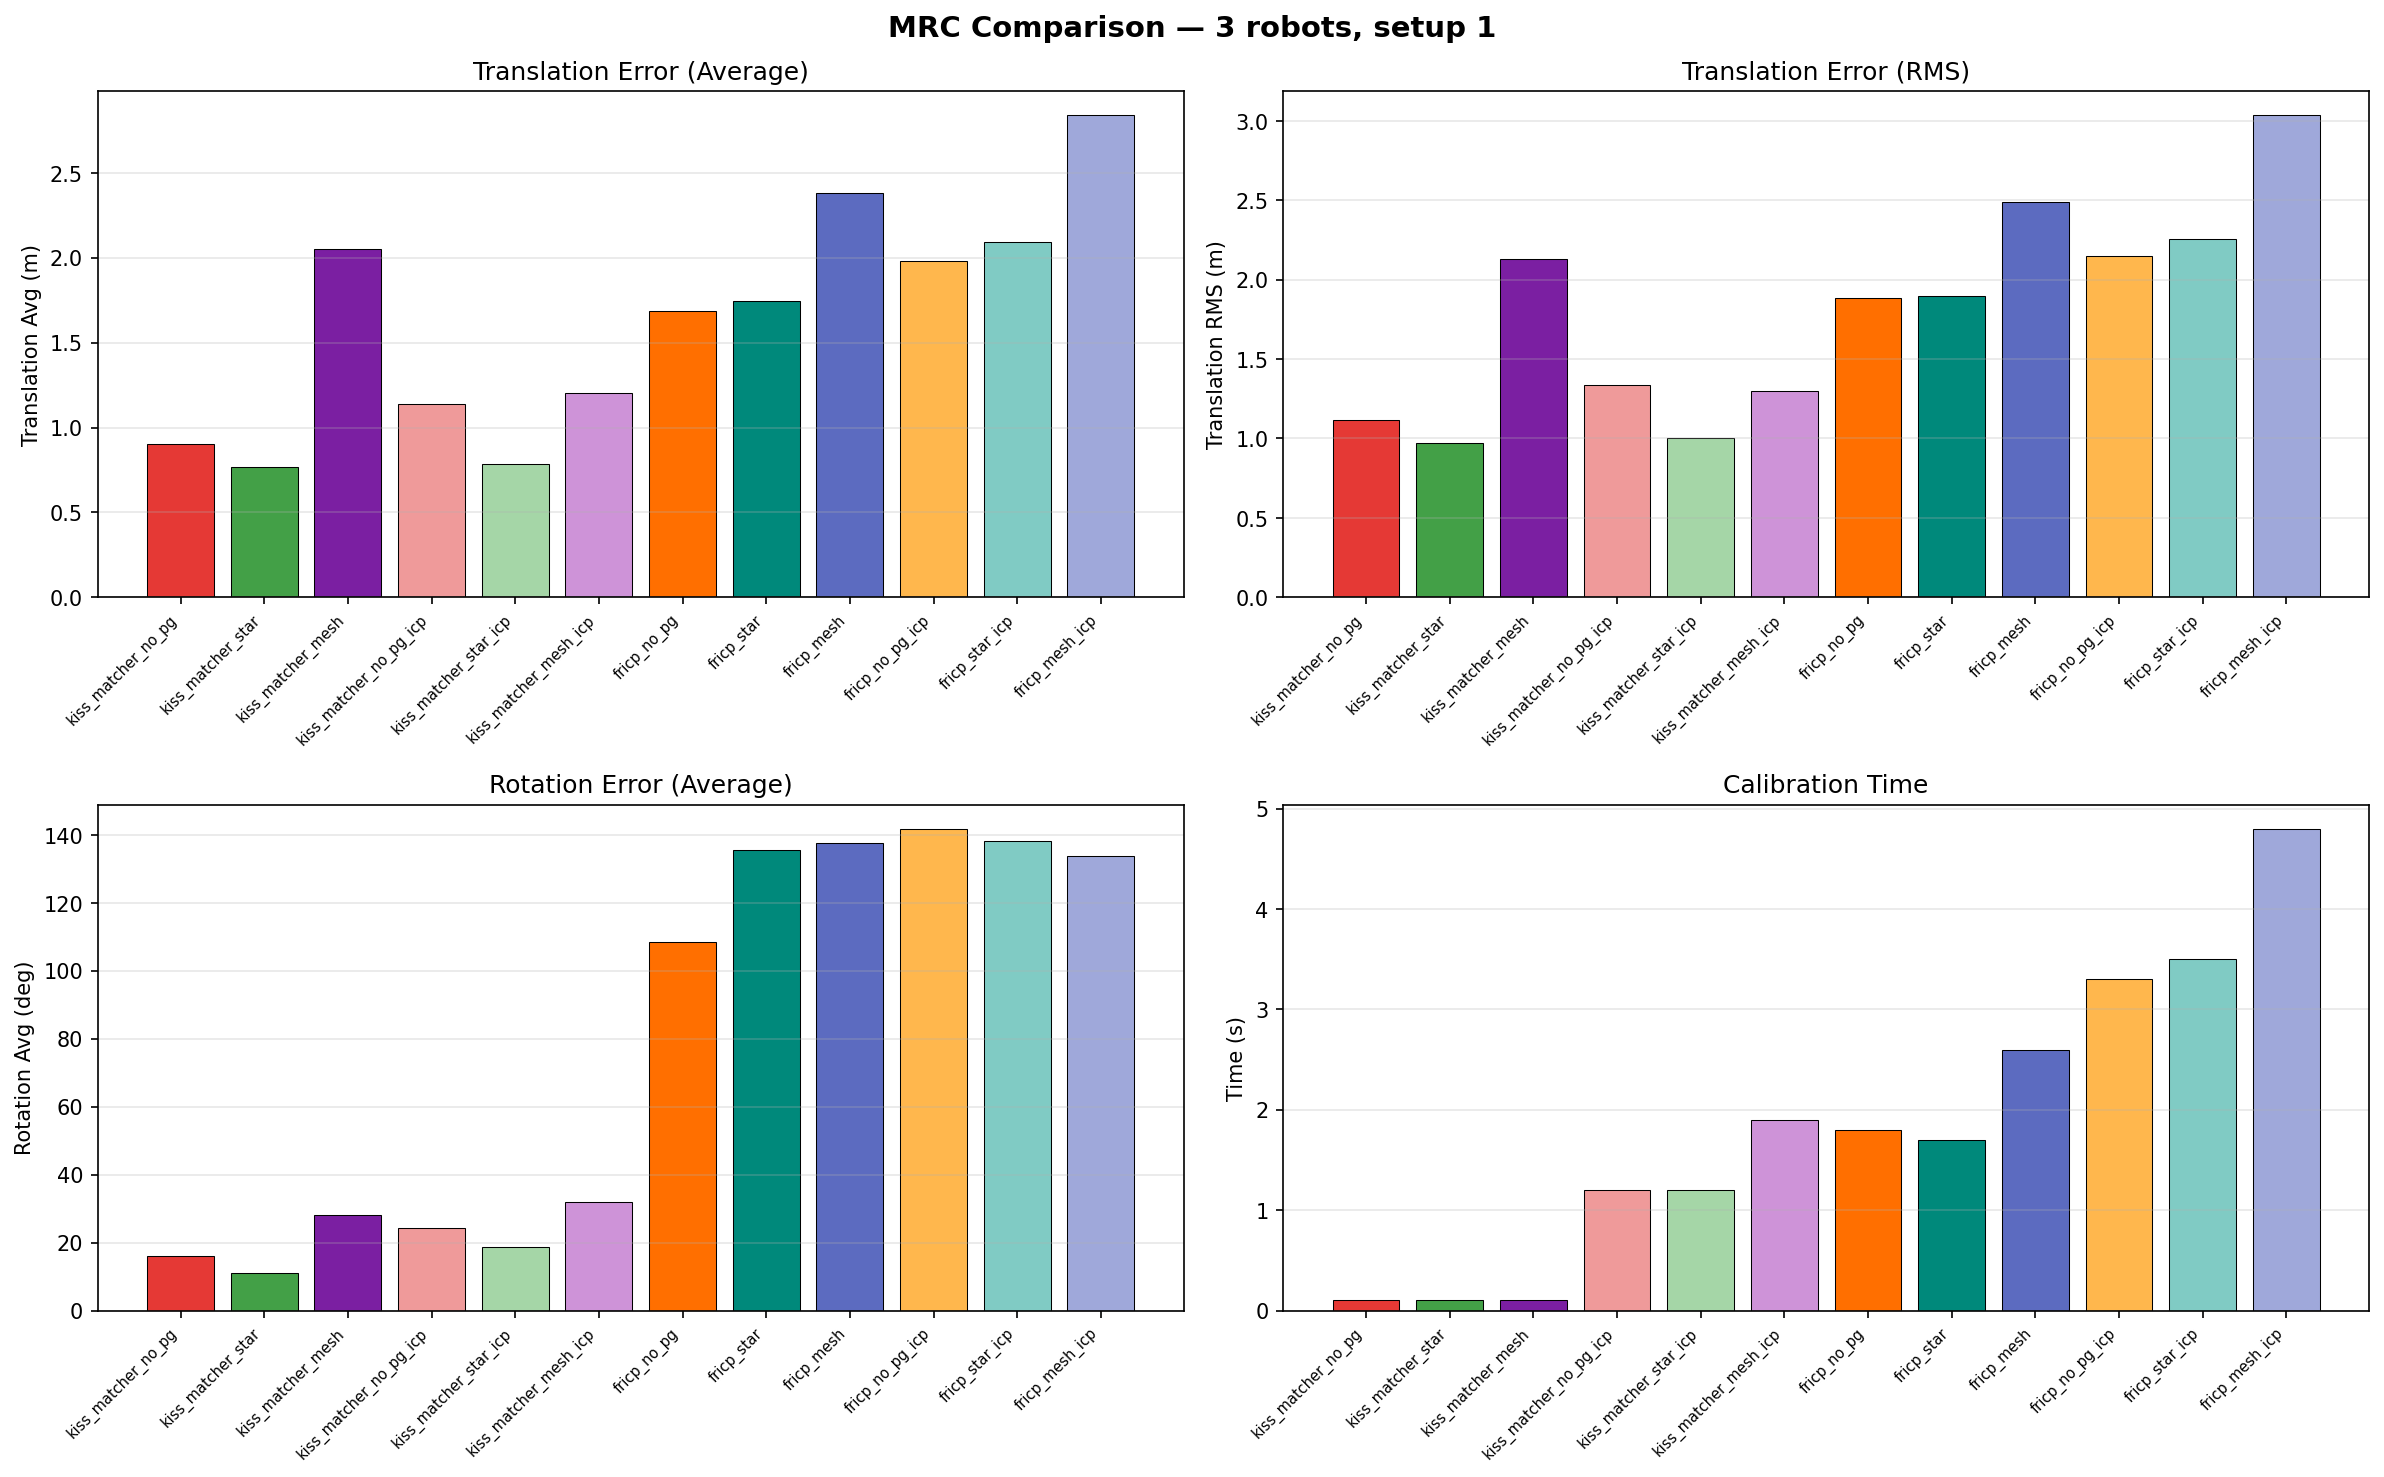
\includegraphics[width=0.95\textwidth]{figures/robots_3_setup_1_bars.png}
    \caption{Configuration comparison --- 3~robots, Setup~1.}
    \label{fig:app_3r_s1_bars}
\end{figure}

\begin{figure}[htbp]
    \centering
    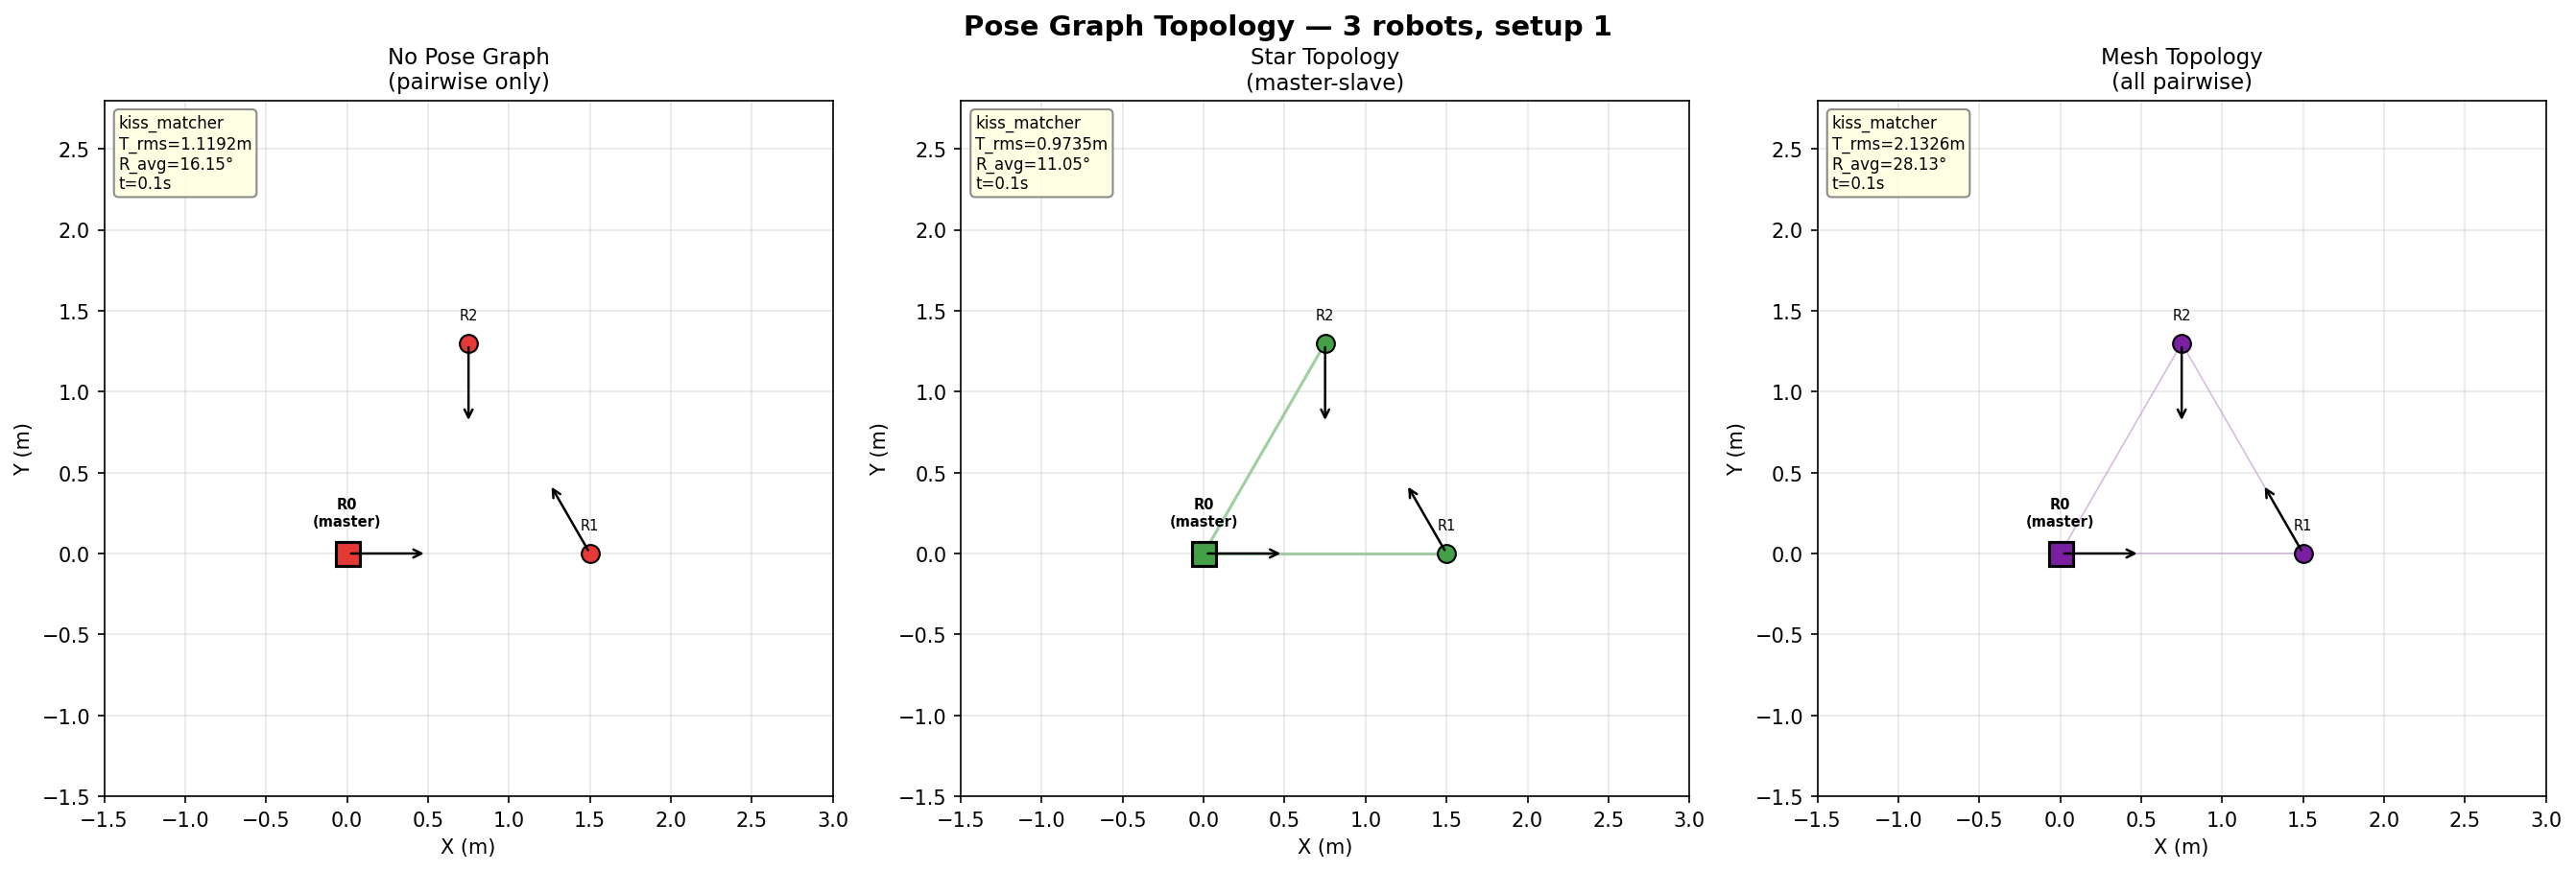
\includegraphics[width=0.7\textwidth]{figures/robots_3_setup_1_pose_graph.png}
    \caption{Pose graph visualization --- 3~robots, Setup~1.}
    \label{fig:app_3r_s1_pg}
\end{figure}

\begin{figure}[htbp]
    \centering
    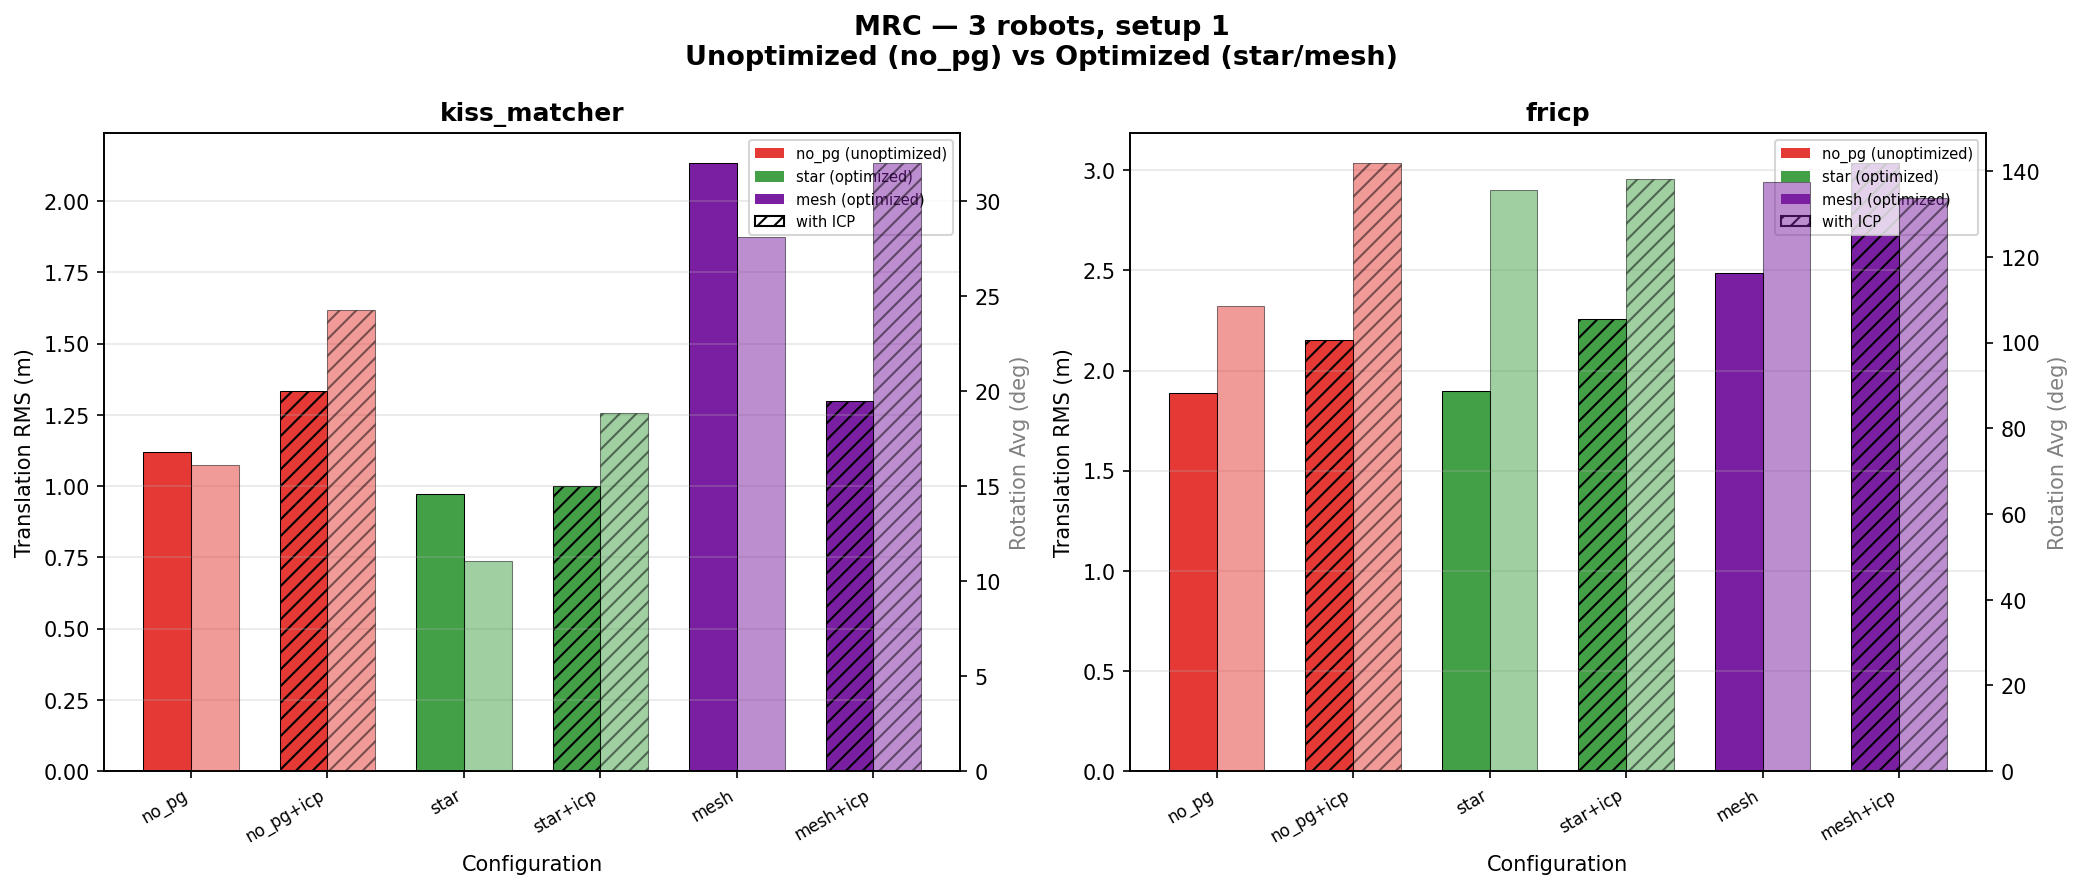
\includegraphics[width=0.95\textwidth]{figures/robots_3_setup_1_unopt_vs_opt.png}
    \caption{Unoptimized vs.\ optimized comparison --- 3~robots, Setup~1.}
    \label{fig:app_3r_s1_unopt}
\end{figure}

%% --- Setup 2 ---
\subsection{Setup~2: Wide Equilateral Triangle}

\begin{table}[htbp]
    \centering
    \caption{3~robots, Setup~2 --- wide equilateral triangle
             (overlap: 55.6\%).}
    \label{tab:app_3r_s2}
    \small
    \begin{tabular}{l r r r r r}
        \toprule
        \textbf{Configuration}
            & $\bar{e}_t$ [m]
            & $e_t^\mathrm{RMS}$ [m]
            & $\bar{e}_r$ [deg]
            & Ovlp [\%]
            & $t$ [s] \\
        \midrule
        \multicolumn{6}{l}{\textit{KISS-Matcher}} \\
        \quad no PG         & 5.04 & 5.27 &  89.7 & 55.6 & 0.1 \\
        \quad star PG       & 6.63 & 7.17 & 115.9 & 55.6 & 0.1 \\
        \quad mesh PG       & 6.46 & 7.04 & 142.7 & 55.6 & 0.1 \\
        \quad no PG + ICP   & 5.72 & 6.14 & 134.4 & 55.6 & 1.1 \\
        \quad star PG + ICP & 5.72 & 6.74 & 136.4 & 55.6 & 0.7 \\
        \quad mesh PG + ICP & 6.31 & 7.07 & 133.9 & 55.6 & 1.0 \\
        \midrule
        \multicolumn{6}{l}{\textit{FRICP}} \\
        \quad no PG         & 5.65 & 6.11 & 154.6 & 55.6 & 1.9 \\
        \quad star PG       & 5.29 & 5.63 & 153.4 & 55.6 & 1.8 \\
        \quad mesh PG       & 6.53 & 6.66 & 150.3 & 55.6 & 2.5 \\
        \quad no PG + ICP   & 6.00 & 6.27 & 162.3 & 55.6 & 3.4 \\
        \quad star PG + ICP & 6.03 & 6.44 & 148.7 & 55.6 & 3.1 \\
        \quad mesh PG + ICP & 6.90 & 7.06 & 141.9 & 55.6 & 4.7 \\
        \bottomrule
    \end{tabular}
\end{table}

\begin{figure}[htbp]
    \centering
    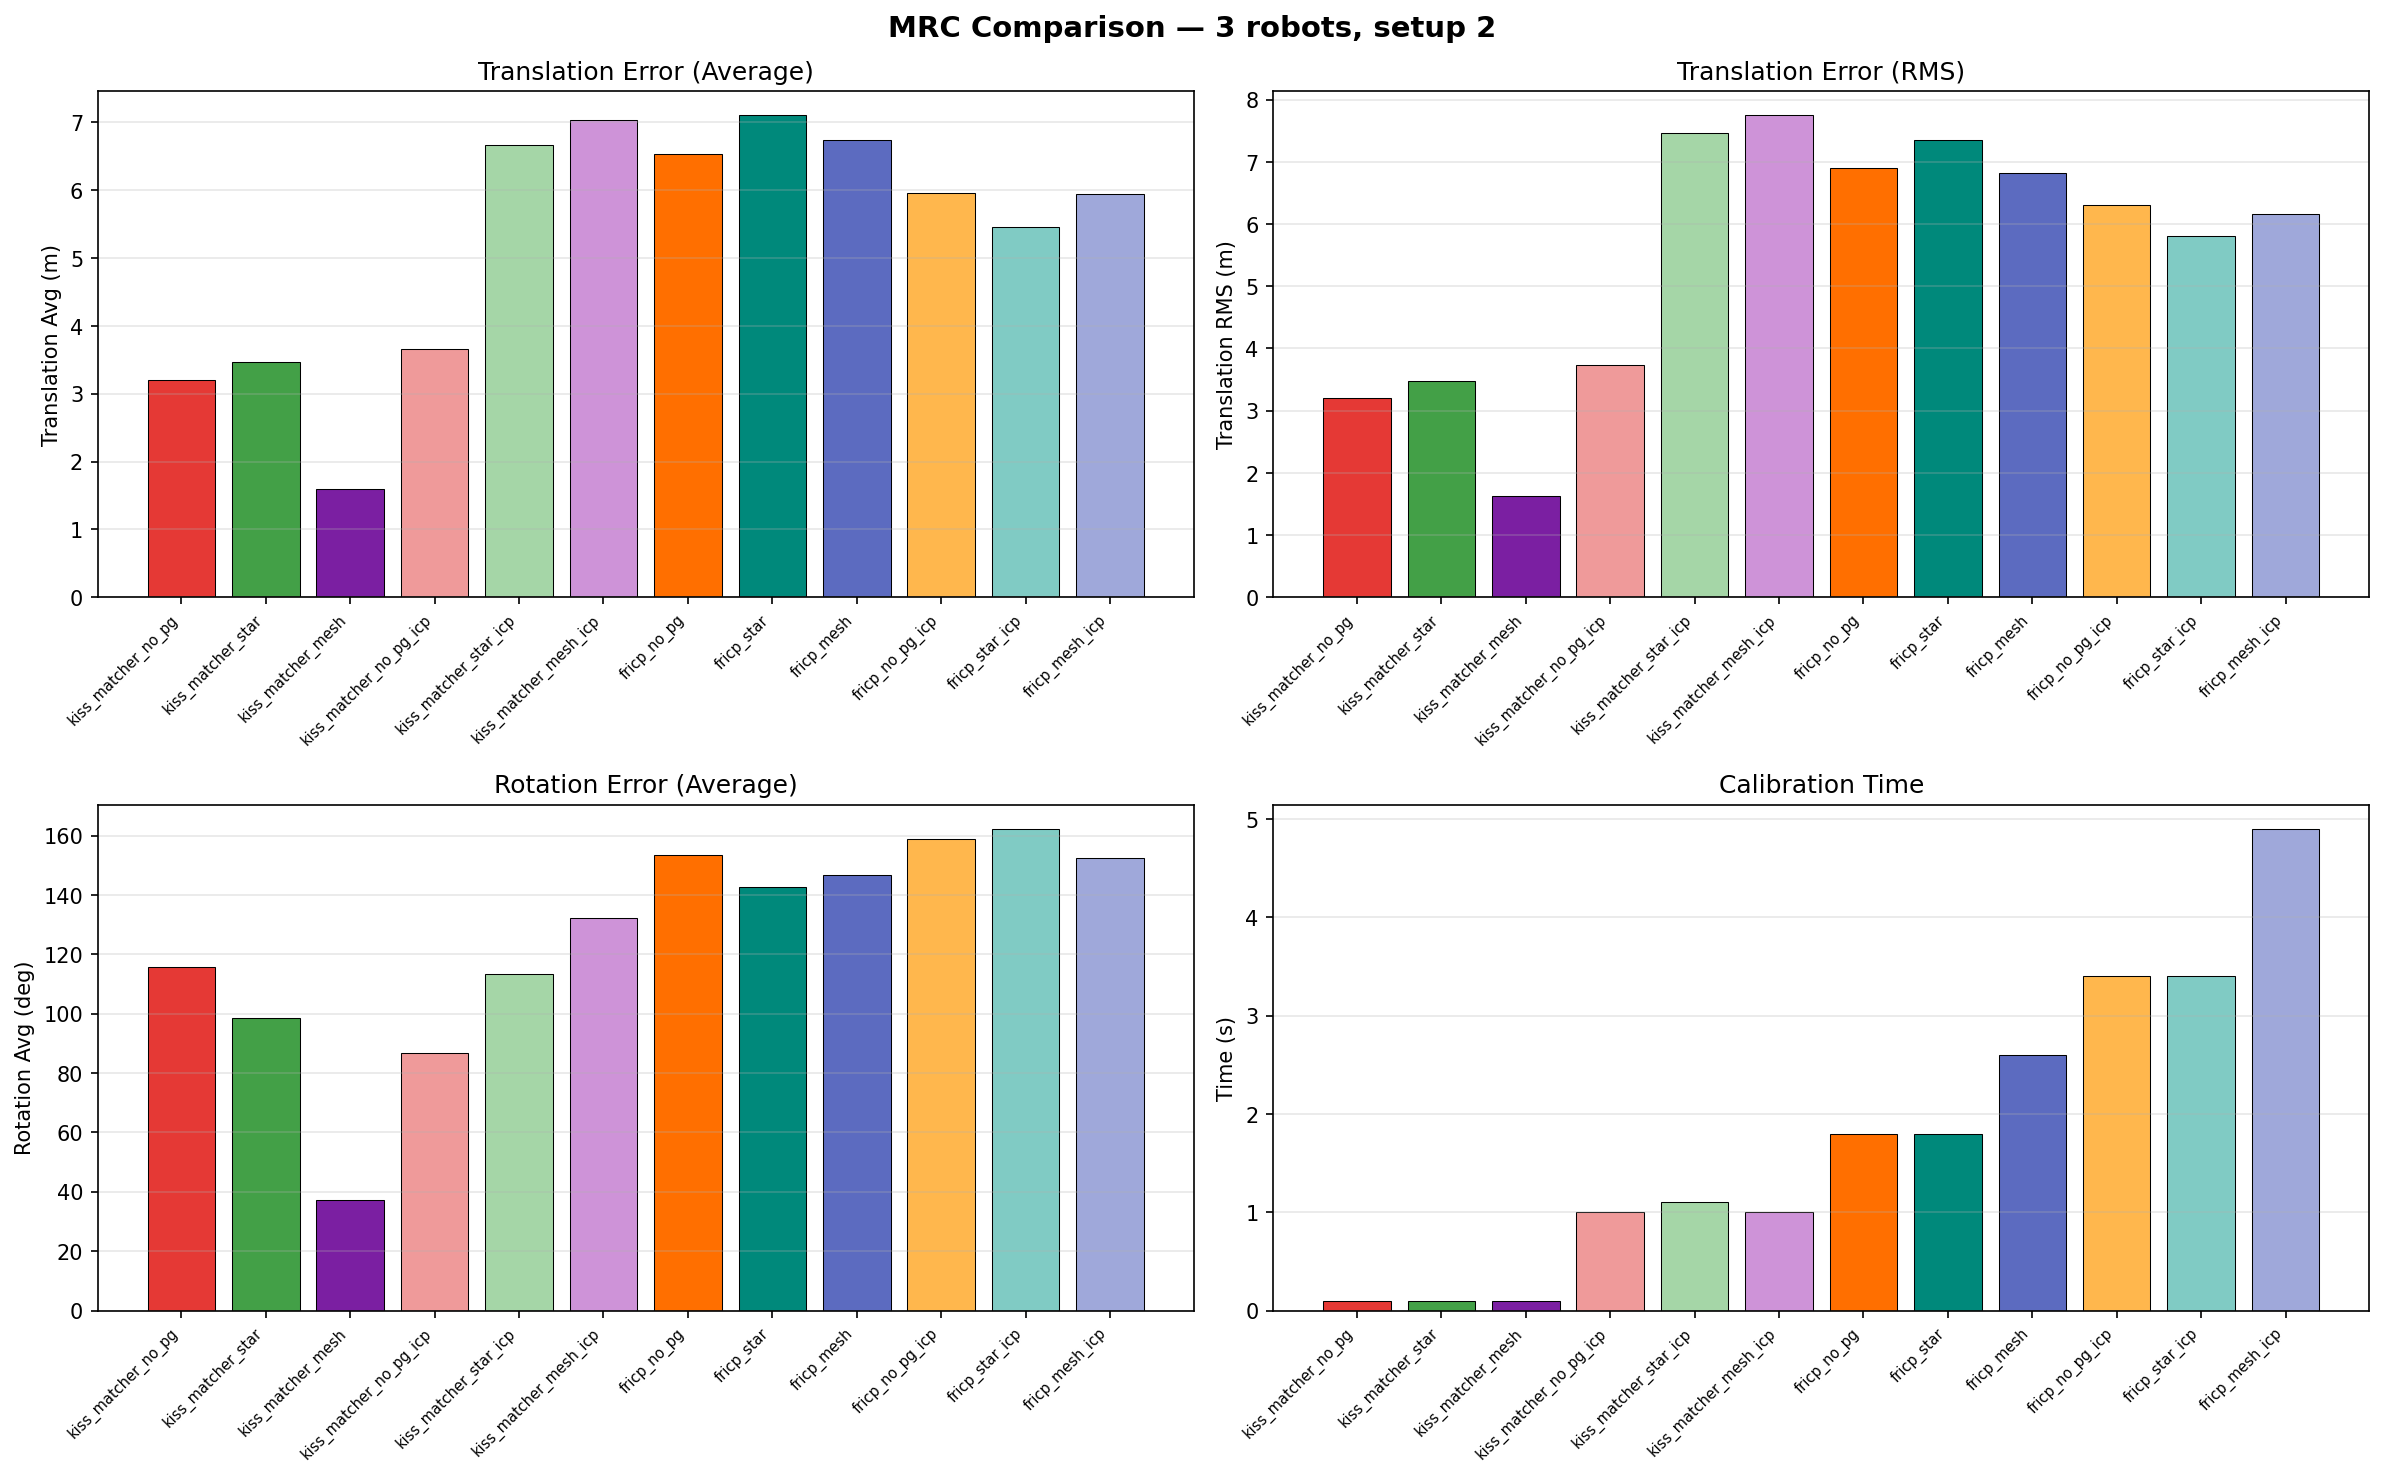
\includegraphics[width=0.95\textwidth]{figures/robots_3_setup_2_bars.png}
    \caption{Configuration comparison --- 3~robots, Setup~2.}
    \label{fig:app_3r_s2_bars}
\end{figure}

\begin{figure}[htbp]
    \centering
    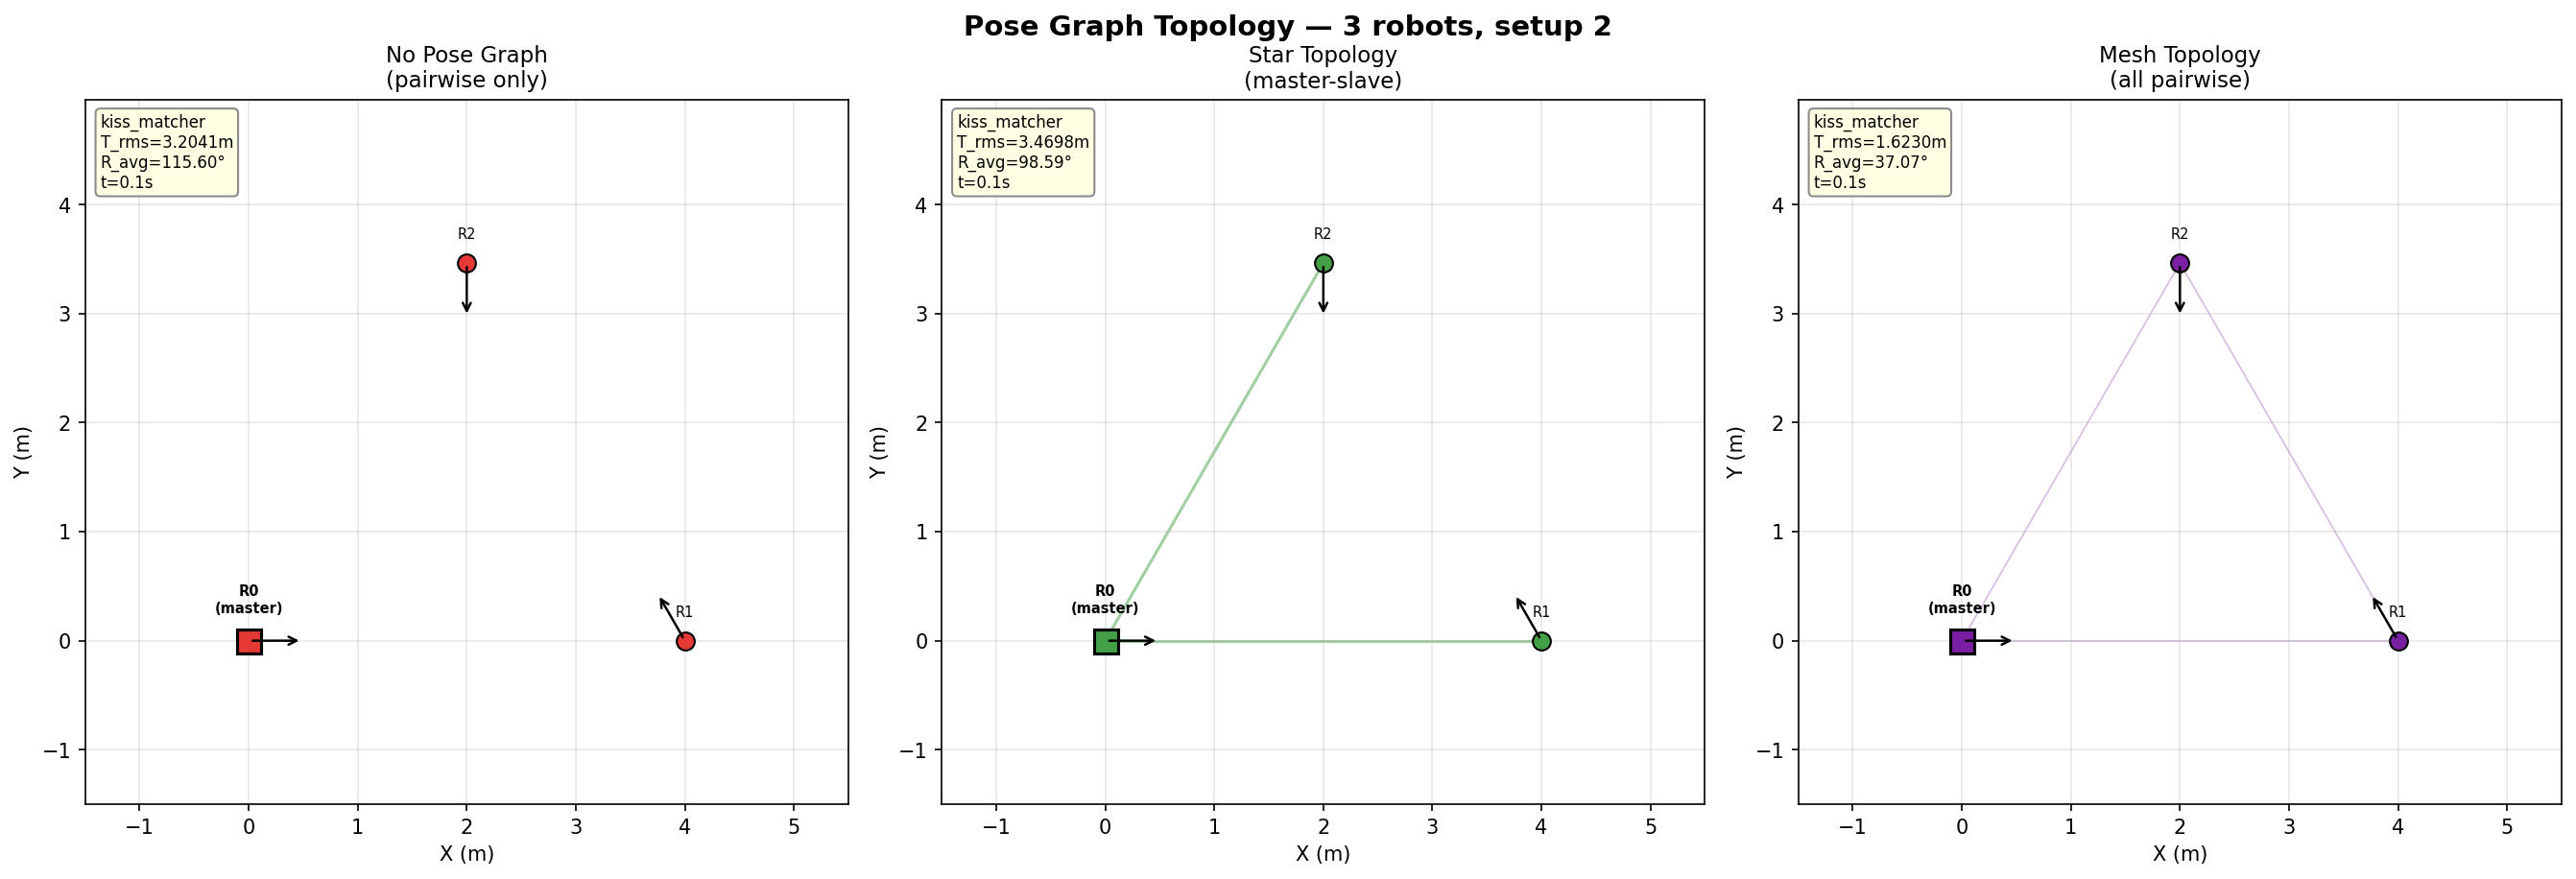
\includegraphics[width=0.7\textwidth]{figures/robots_3_setup_2_pose_graph.png}
    \caption{Pose graph visualization --- 3~robots, Setup~2.}
    \label{fig:app_3r_s2_pg}
\end{figure}

\begin{figure}[htbp]
    \centering
    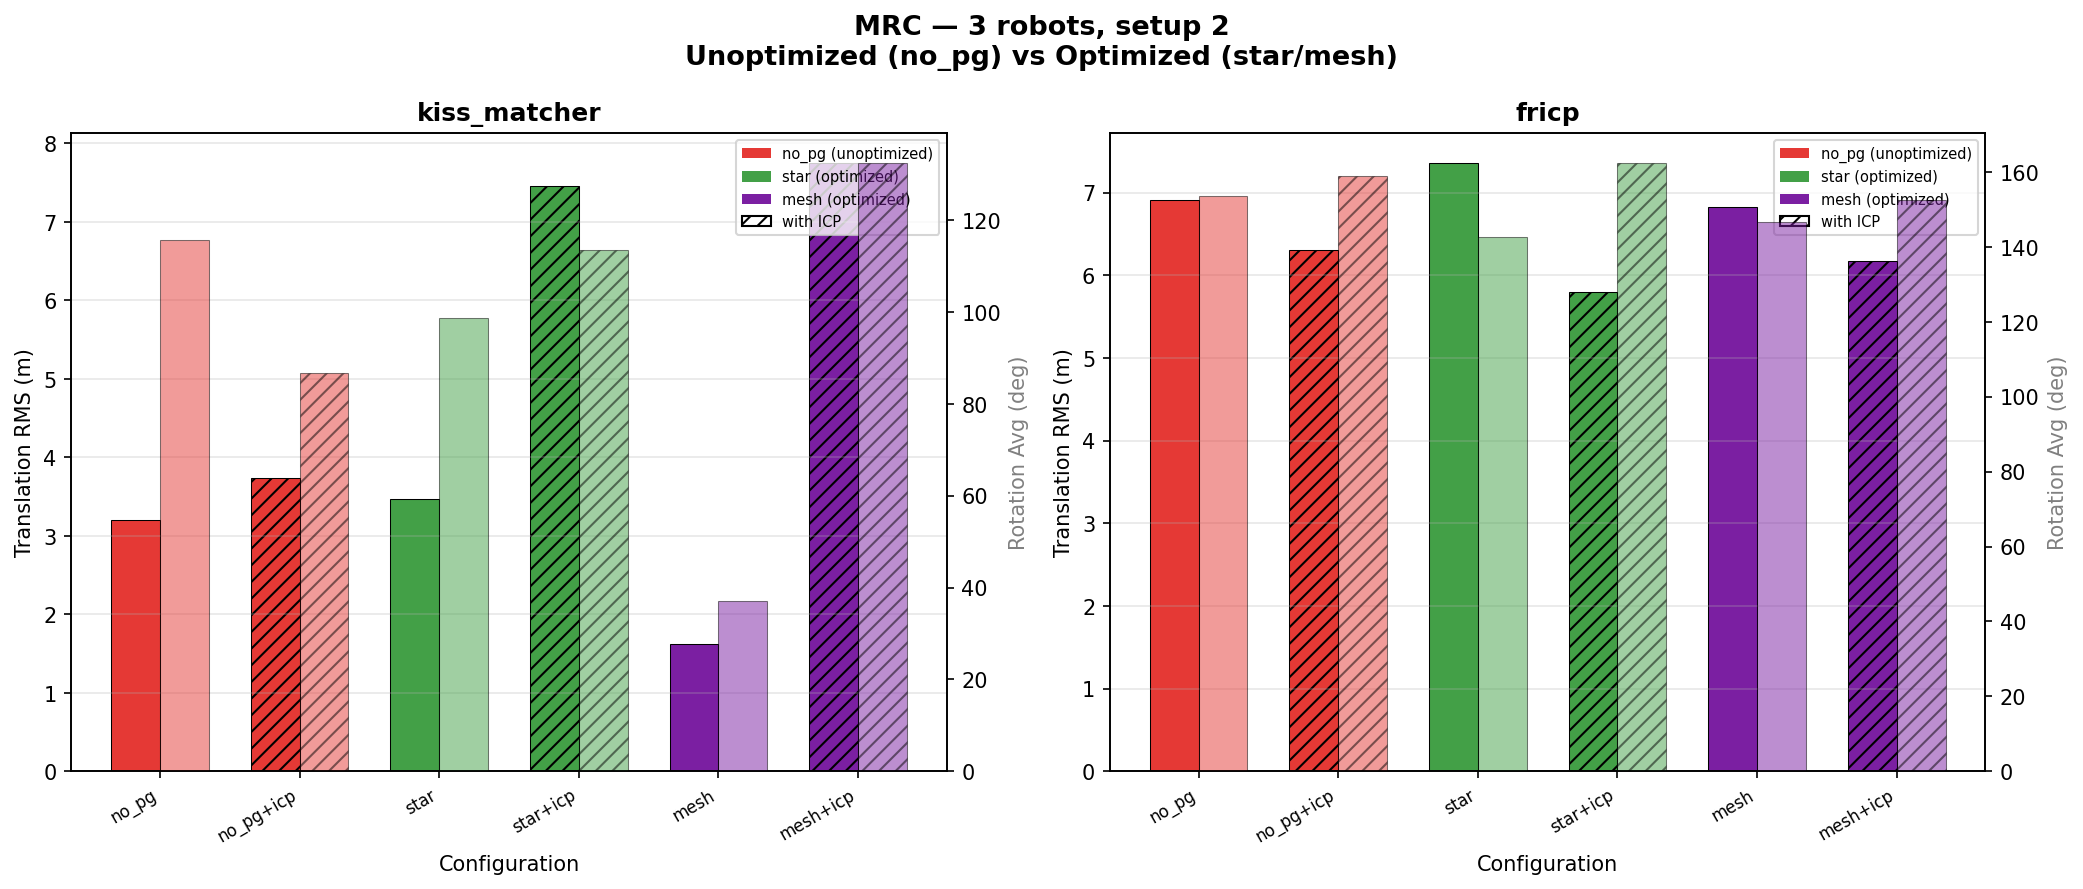
\includegraphics[width=0.95\textwidth]{figures/robots_3_setup_2_unopt_vs_opt.png}
    \caption{Unoptimized vs.\ optimized comparison --- 3~robots, Setup~2.}
    \label{fig:app_3r_s2_unopt}
\end{figure}

%% --- Setup 3 ---
\subsection{Setup~3: Line Formation}

\begin{table}[htbp]
    \centering
    \caption{3~robots, Setup~3 --- line formation
             (overlap: 64.2\%).}
    \label{tab:app_3r_s3}
    \small
    \begin{tabular}{l r r r r r}
        \toprule
        \textbf{Configuration}
            & $\bar{e}_t$ [m]
            & $e_t^\mathrm{RMS}$ [m]
            & $\bar{e}_r$ [deg]
            & Ovlp [\%]
            & $t$ [s] \\
        \midrule
        \multicolumn{6}{l}{\textit{KISS-Matcher}} \\
        \quad no PG         & 1.49 & 2.04 &  61.9 & 64.2 & 0.1 \\
        \quad star PG       & 1.35 & 1.74 &  53.5 & 64.2 & 0.1 \\
        \quad mesh PG       & 1.61 & 1.98 &  29.7 & 64.2 & 0.1 \\
        \quad no PG + ICP   & 1.78 & 2.39 &  53.9 & 64.2 & 1.5 \\
        \quad star PG + ICP & 2.32 & 3.21 &  88.4 & 64.2 & 1.6 \\
        \quad mesh PG + ICP & 2.21 & 3.04 & 125.3 & 64.2 & 2.1 \\
        \midrule
        \multicolumn{6}{l}{\textit{FRICP}} \\
        \quad no PG         & 3.73 & 4.18 & 131.8 & 64.2 & 1.5 \\
        \quad star PG       & 4.25 & 4.56 & 133.9 & 64.2 & 1.6 \\
        \quad mesh PG       & 4.42 & 4.68 & 134.7 & 64.2 & 2.4 \\
        \quad no PG + ICP   & 3.94 & 4.49 & 135.4 & 64.2 & 3.0 \\
        \quad star PG + ICP & 3.81 & 4.46 & 135.9 & 64.2 & 3.0 \\
        \quad mesh PG + ICP & 3.52 & 4.35 & 135.5 & 64.2 & 4.7 \\
        \bottomrule
    \end{tabular}
\end{table}

\begin{figure}[htbp]
    \centering
    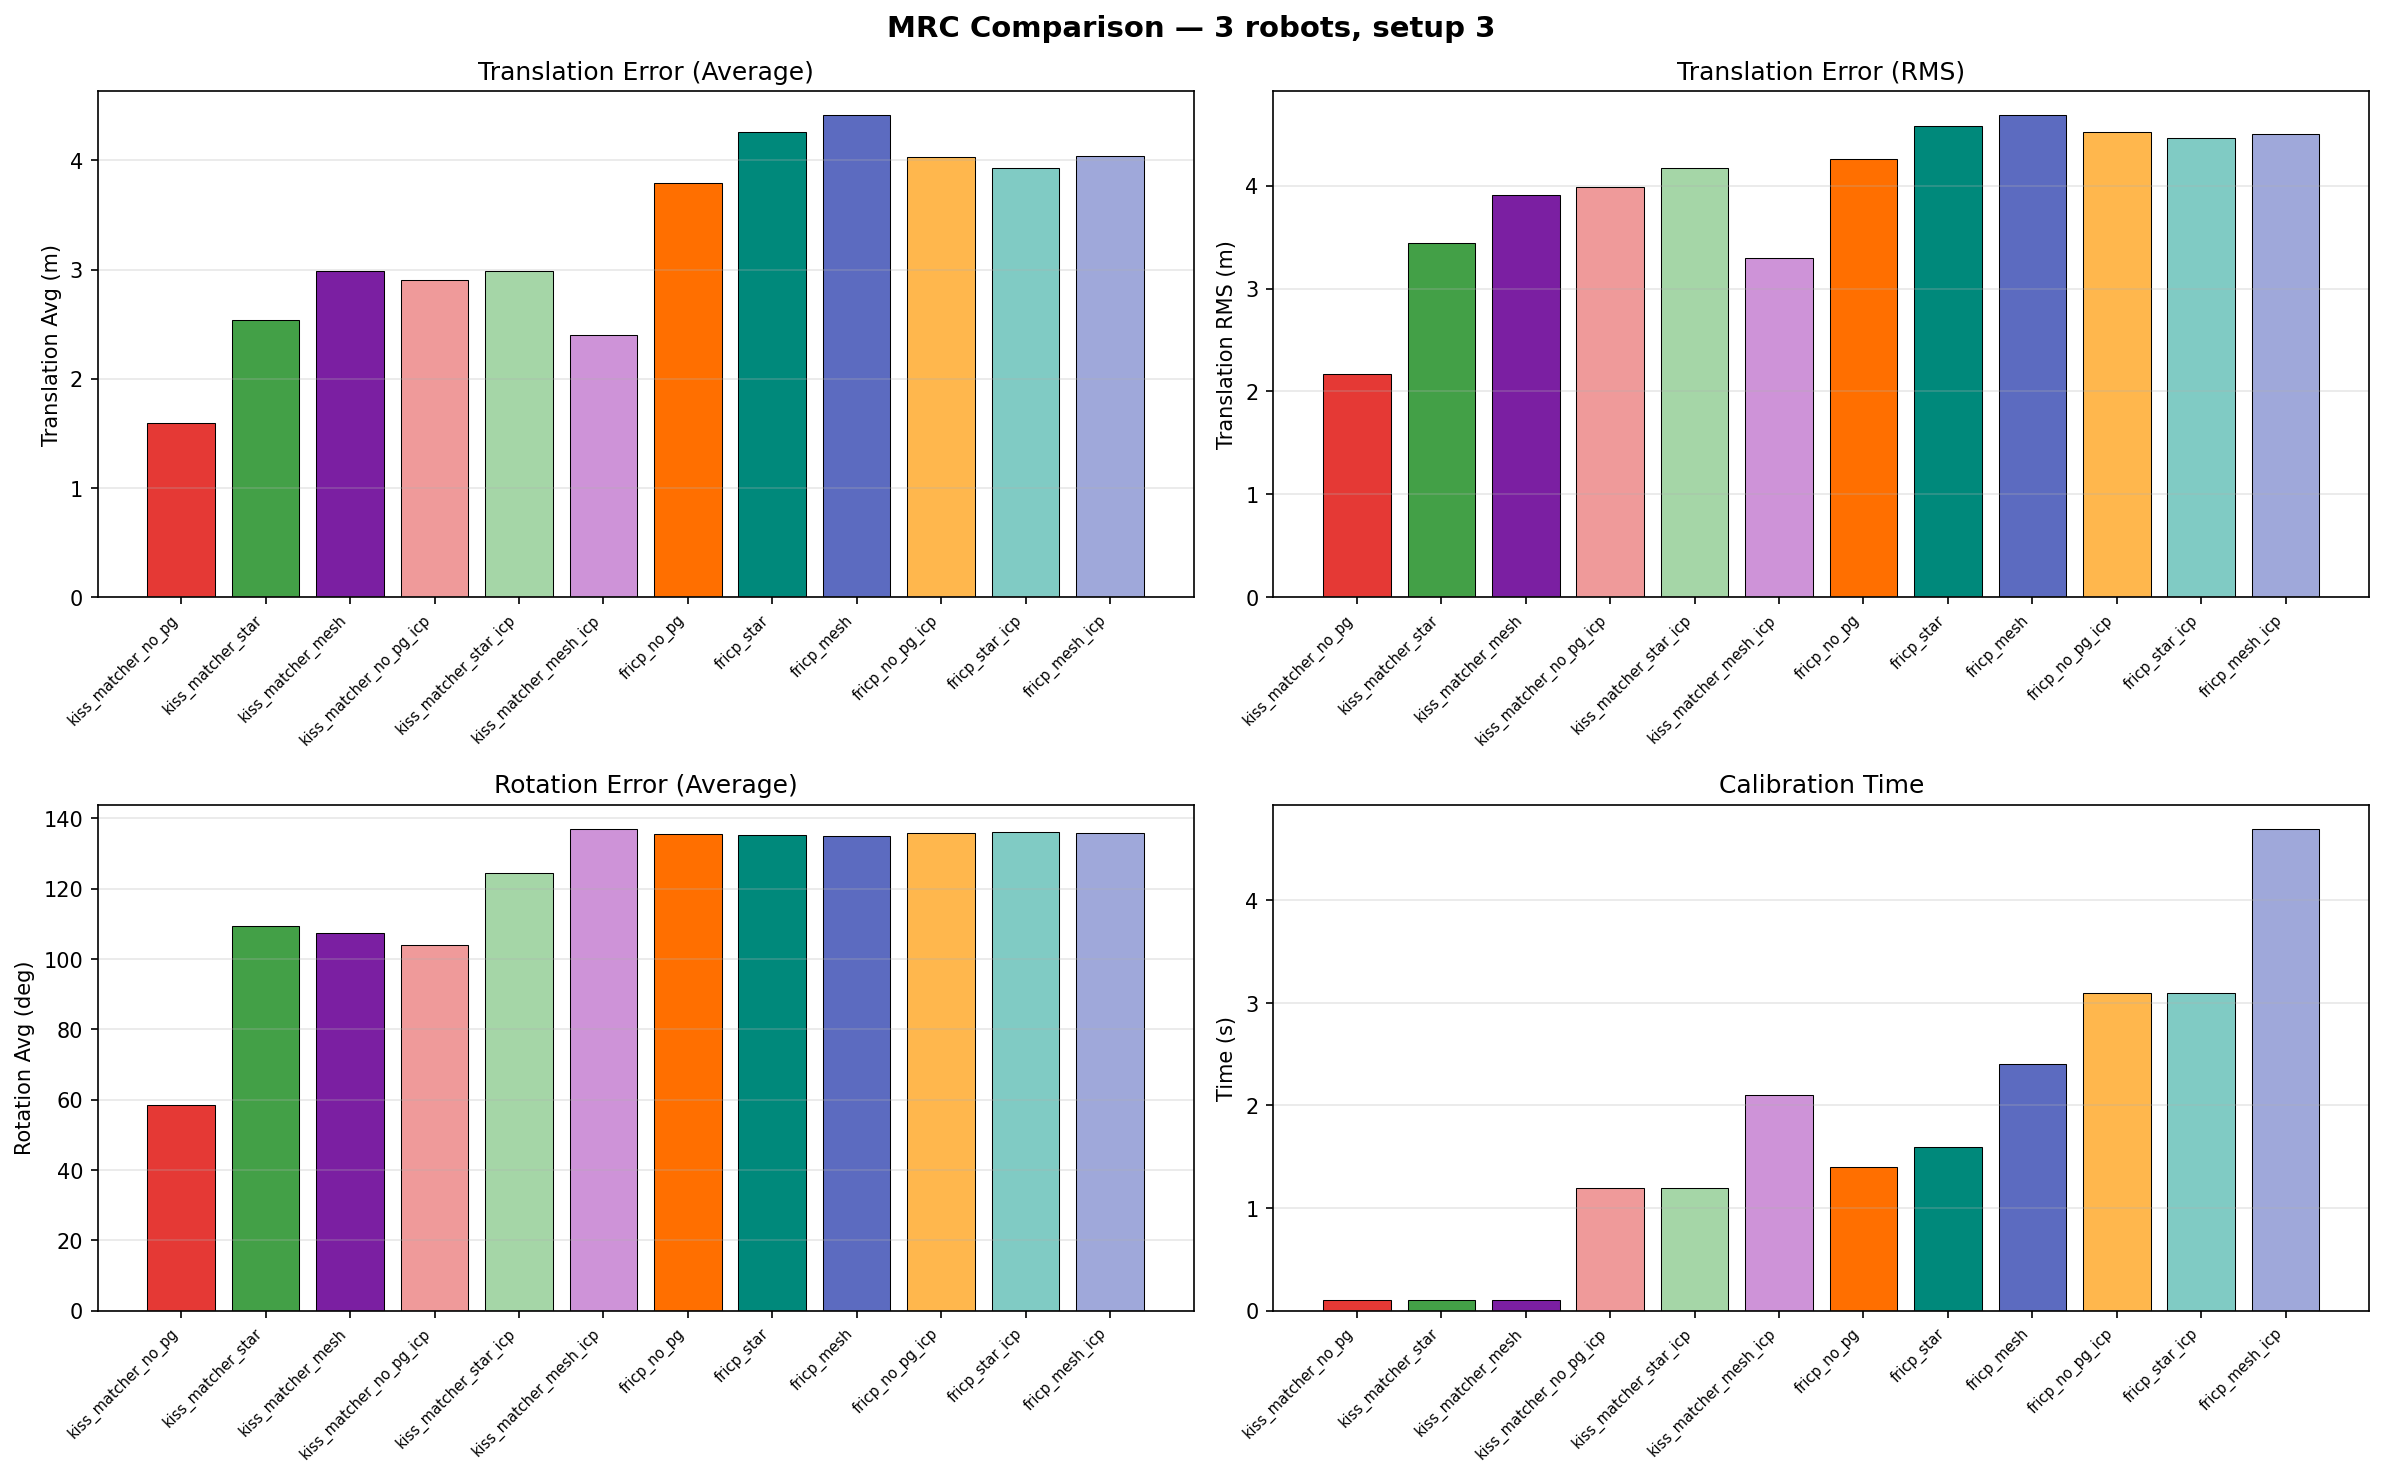
\includegraphics[width=0.95\textwidth]{figures/robots_3_setup_3_bars.png}
    \caption{Configuration comparison --- 3~robots, Setup~3.}
    \label{fig:app_3r_s3_bars}
\end{figure}

\begin{figure}[htbp]
    \centering
    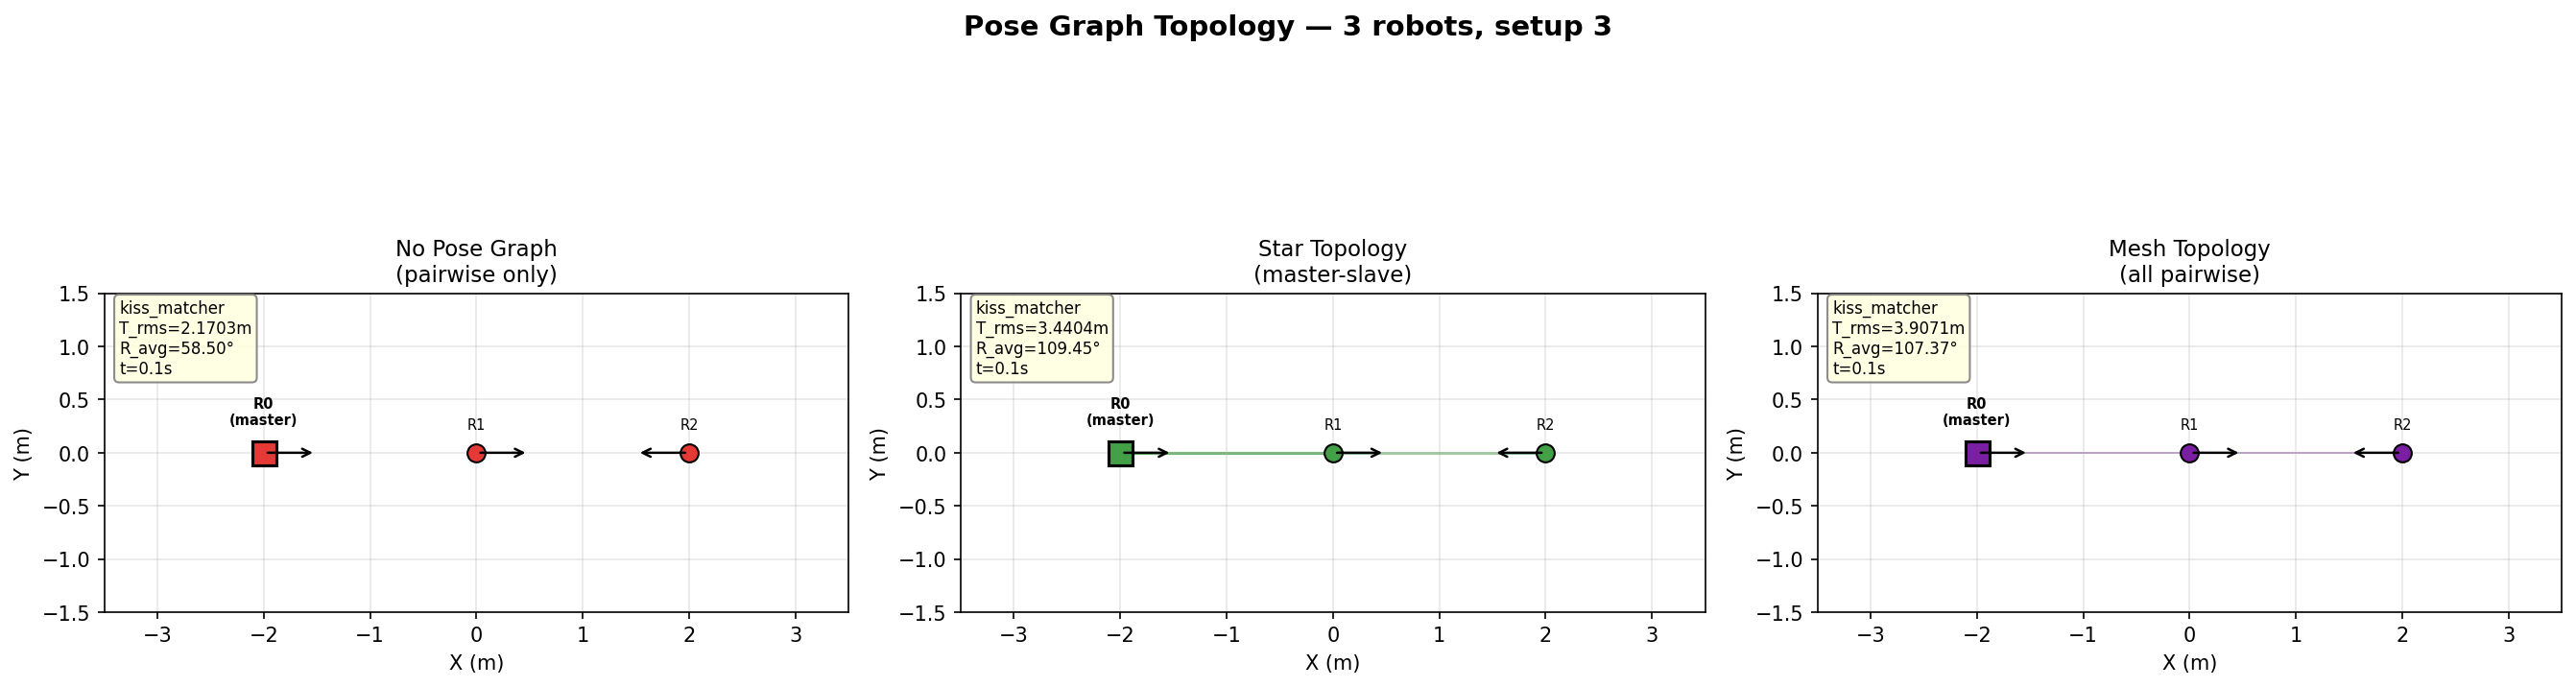
\includegraphics[width=0.7\textwidth]{figures/robots_3_setup_3_pose_graph.png}
    \caption{Pose graph visualization --- 3~robots, Setup~3.}
    \label{fig:app_3r_s3_pg}
\end{figure}

\begin{figure}[htbp]
    \centering
    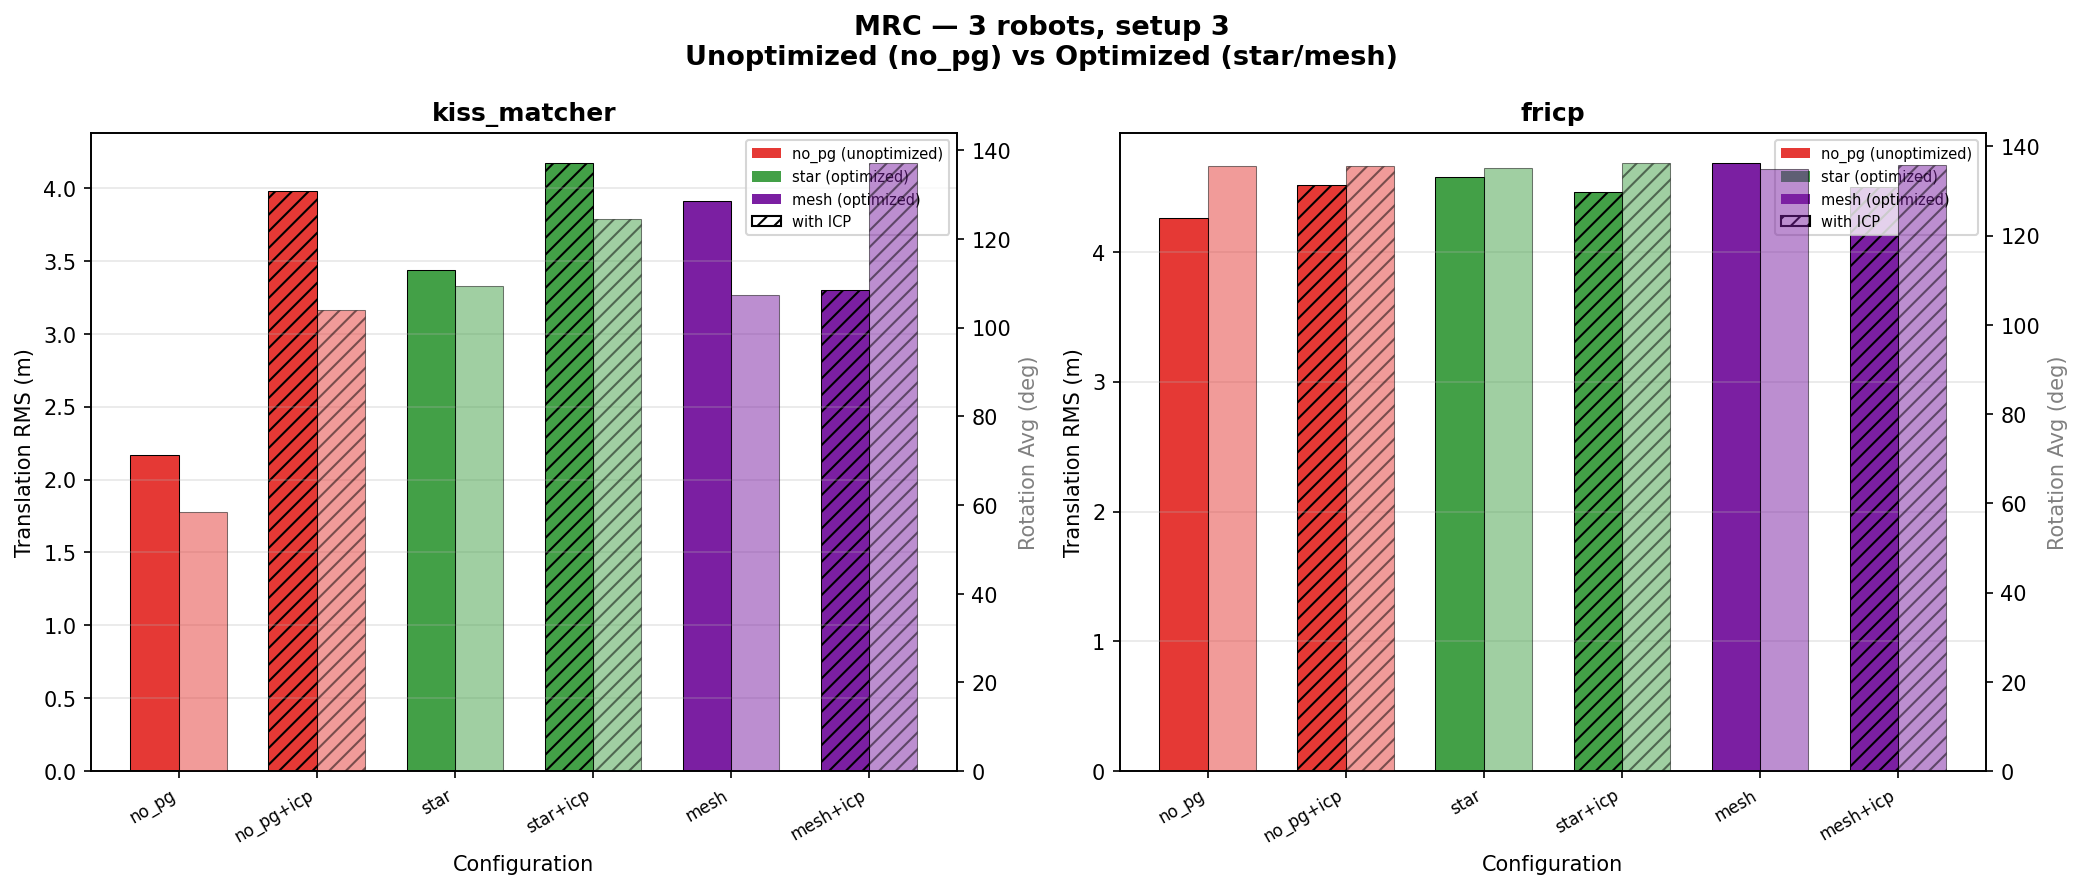
\includegraphics[width=0.95\textwidth]{figures/robots_3_setup_3_unopt_vs_opt.png}
    \caption{Unoptimized vs.\ optimized comparison --- 3~robots, Setup~3.}
    \label{fig:app_3r_s3_unopt}
\end{figure}

%% --- Setup 4 ---
\subsection{Setup~4: Structured Composite}

\begin{table}[htbp]
    \centering
    \caption{3~robots, Setup~4 --- structured composite
             (overlap: 59.3\%).}
    \label{tab:app_3r_s4}
    \small
    \begin{tabular}{l r r r r r}
        \toprule
        \textbf{Configuration}
            & $\bar{e}_t$ [m]
            & $e_t^\mathrm{RMS}$ [m]
            & $\bar{e}_r$ [deg]
            & Ovlp [\%]
            & $t$ [s] \\
        \midrule
        \multicolumn{6}{l}{\textit{KISS-Matcher}} \\
        \quad no PG         & 4.49 & 4.84 &  39.9 & 59.3 & 0.1 \\
        \quad star PG       & 1.73 & 1.85 &  15.5 & 59.3 & 0.1 \\
        \quad mesh PG       & 0.90 & 0.95 &   7.2 & 59.3 & 0.1 \\
        \quad no PG + ICP   & 0.83 & 1.06 &  23.5 & 59.3 & 1.1 \\
        \quad star PG + ICP & 1.74 & 2.10 &  60.9 & 59.3 & 1.0 \\
        \quad mesh PG + ICP & 0.60 & 0.72 &  21.5 & 59.3 & 1.9 \\
        \midrule
        \multicolumn{6}{l}{\textit{FRICP}} \\
        \quad no PG         & 2.31 & 2.79 &  67.2 & 59.3 & 1.8 \\
        \quad star PG       & 3.01 & 3.61 &  78.9 & 59.3 & 1.9 \\
        \quad mesh PG       & 3.88 & 4.12 &  92.1 & 59.3 & 3.1 \\
        \quad no PG + ICP   & 2.85 & 3.56 &  75.9 & 59.3 & 2.9 \\
        \quad star PG + ICP & 2.52 & 3.39 &  70.5 & 59.3 & 2.8 \\
        \quad mesh PG + ICP & 3.04 & 3.76 &  82.1 & 59.3 & 5.2 \\
        \bottomrule
    \end{tabular}
\end{table}

\begin{figure}[htbp]
    \centering
    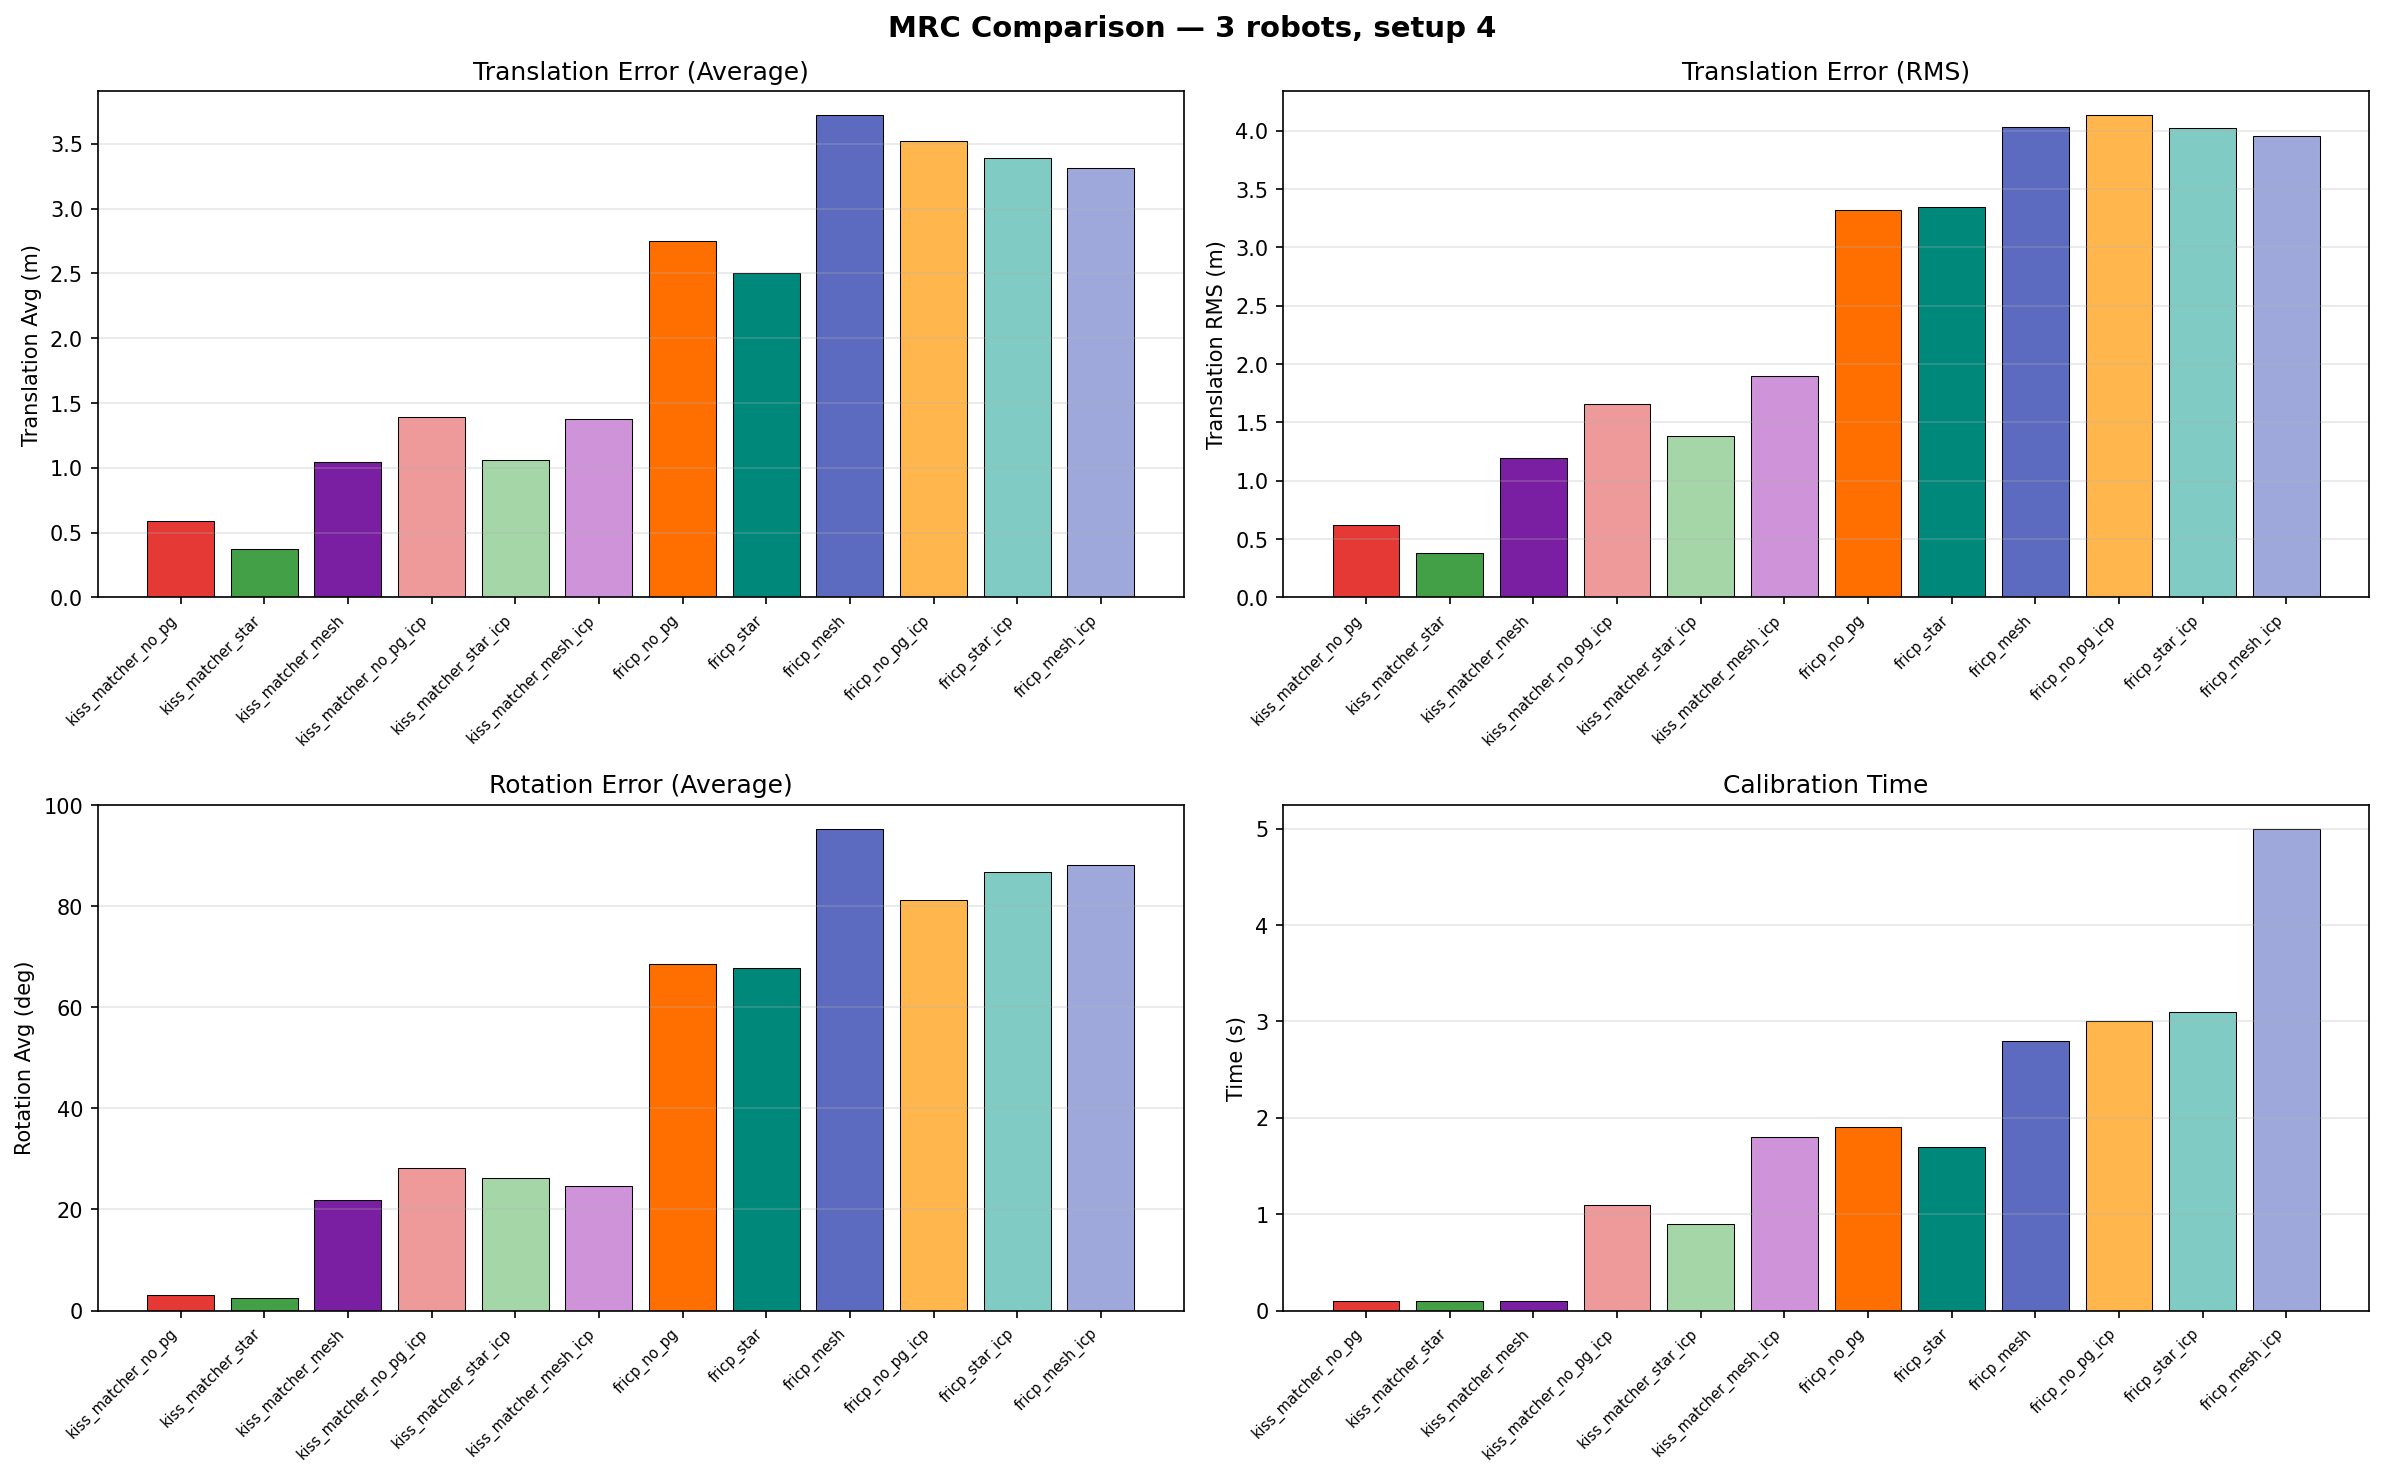
\includegraphics[width=0.95\textwidth]{figures/robots_3_setup_4_bars.png}
    \caption{Configuration comparison --- 3~robots, Setup~4.}
    \label{fig:app_3r_s4_bars}
\end{figure}

\begin{figure}[htbp]
    \centering
    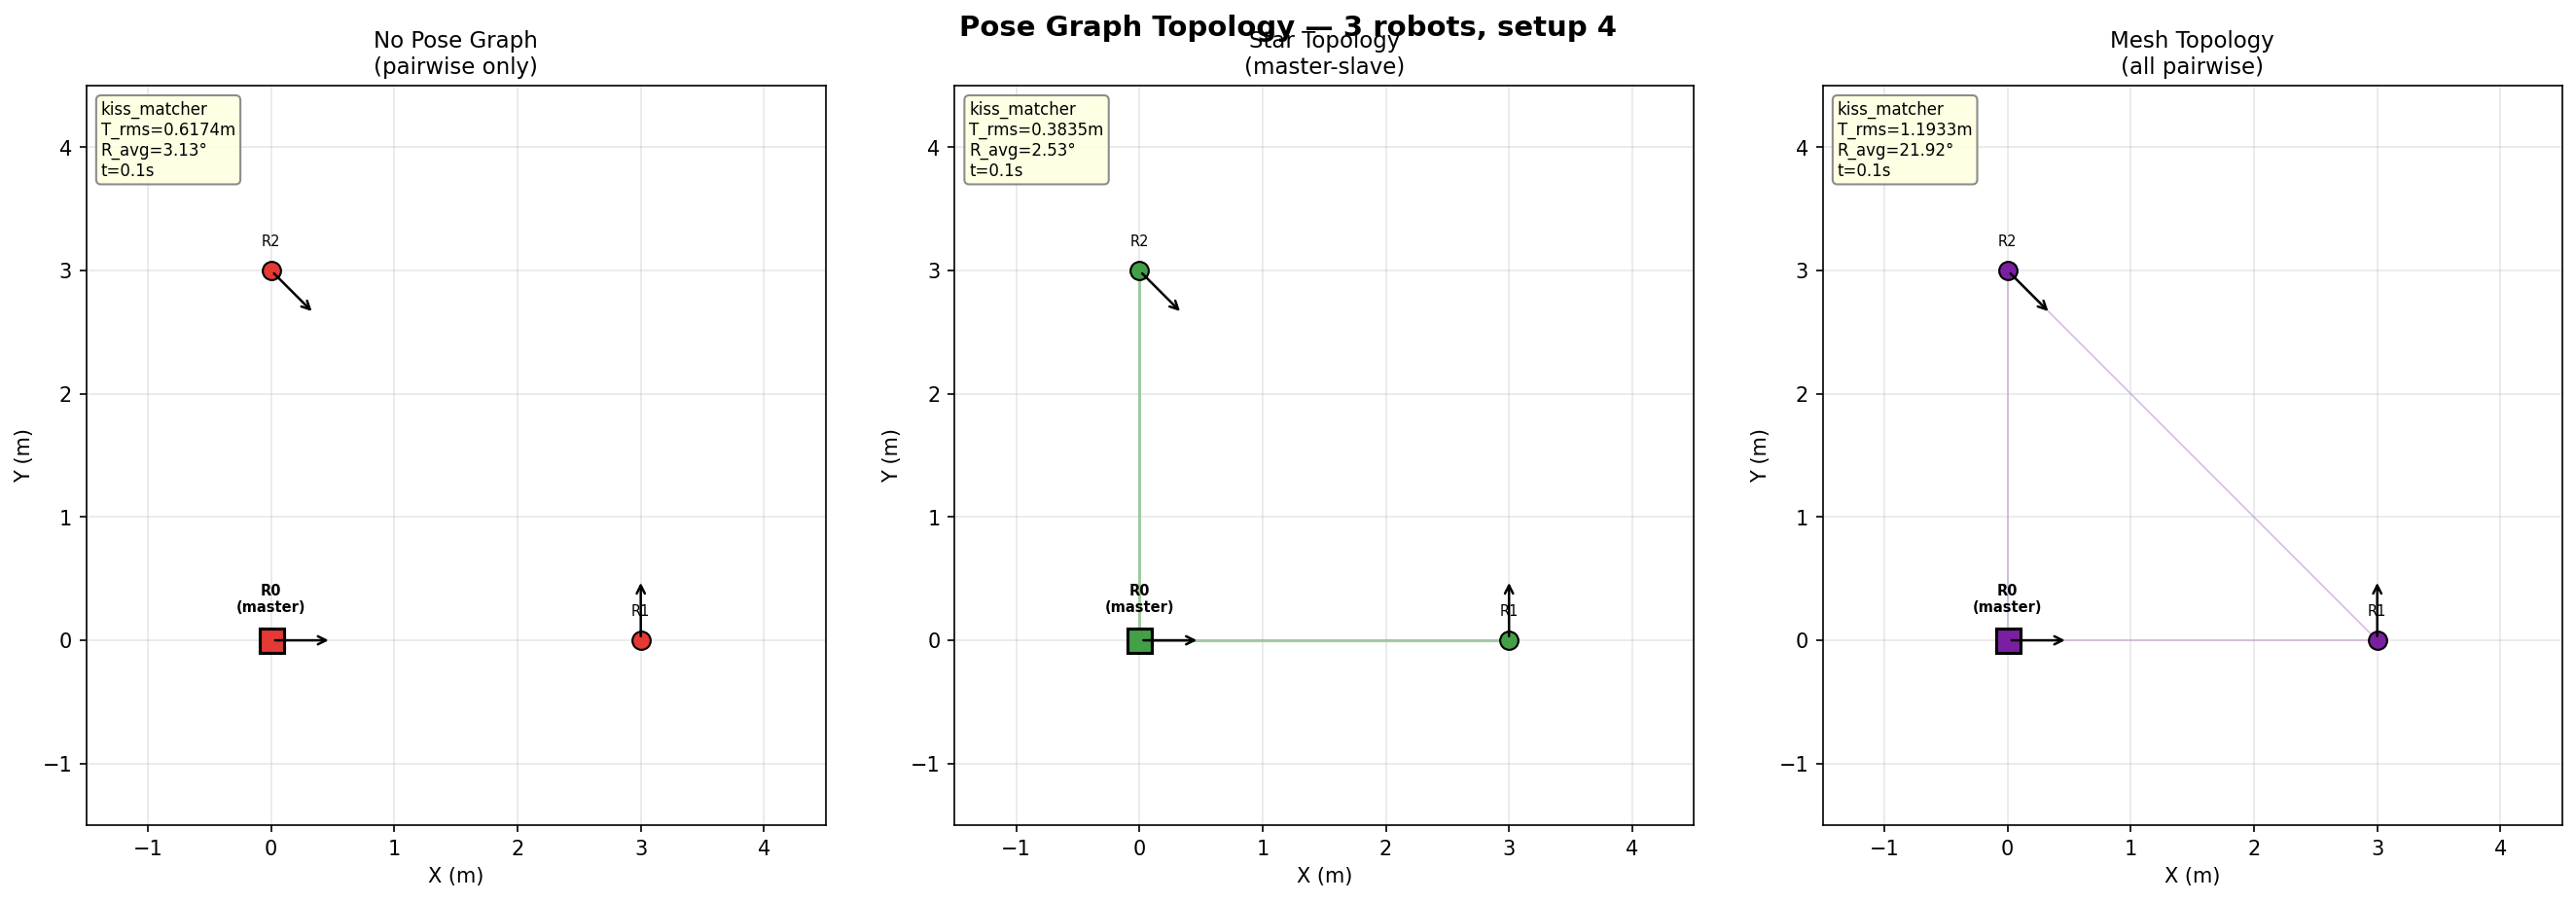
\includegraphics[width=0.7\textwidth]{figures/robots_3_setup_4_pose_graph.png}
    \caption{Pose graph visualization --- 3~robots, Setup~4.}
    \label{fig:app_3r_s4_pg}
\end{figure}

\begin{figure}[htbp]
    \centering
    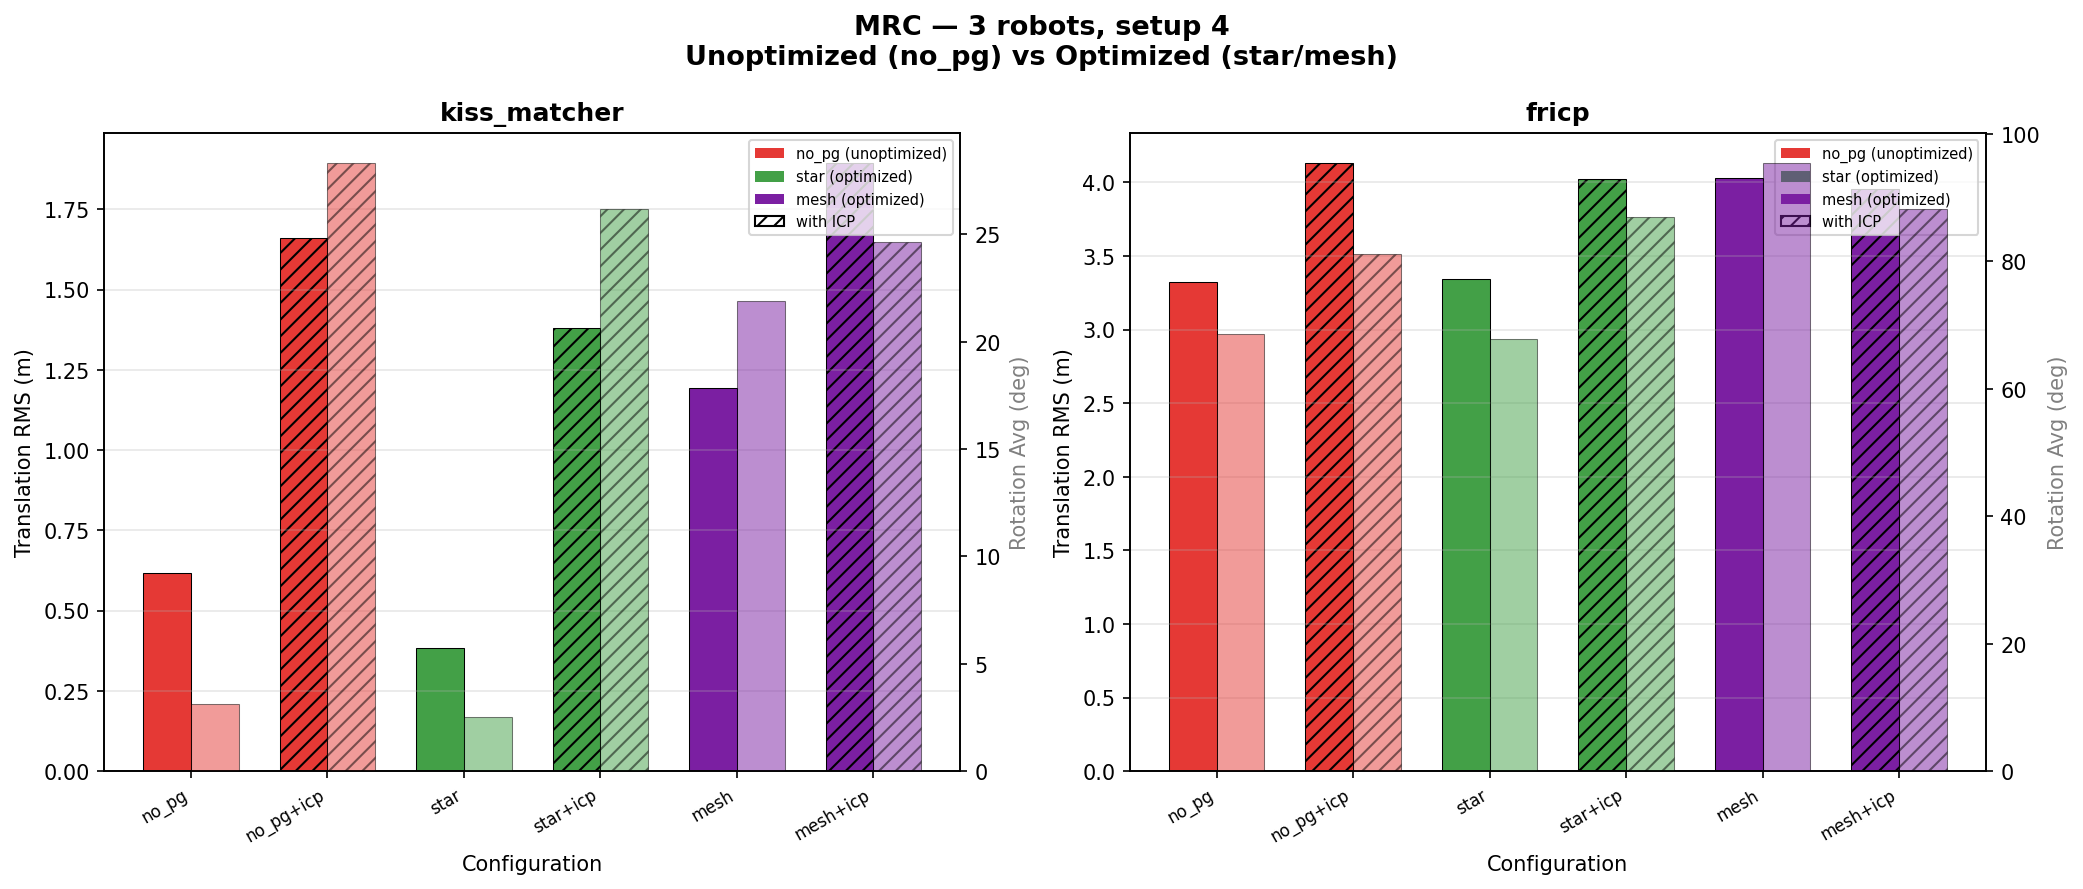
\includegraphics[width=0.95\textwidth]{figures/robots_3_setup_4_unopt_vs_opt.png}
    \caption{Unoptimized vs.\ optimized comparison --- 3~robots, Setup~4.}
    \label{fig:app_3r_s4_unopt}
\end{figure}

%% --- Setup 5 ---
\subsection{Setup~5: Scattered Asymmetric}

\begin{table}[htbp]
    \centering
    \caption{3~robots, Setup~5 --- scattered asymmetric
             (overlap: 51.4\%).}
    \label{tab:app_3r_s5}
    \small
    \begin{tabular}{l r r r r r}
        \toprule
        \textbf{Configuration}
            & $\bar{e}_t$ [m]
            & $e_t^\mathrm{RMS}$ [m]
            & $\bar{e}_r$ [deg]
            & Ovlp [\%]
            & $t$ [s] \\
        \midrule
        \multicolumn{6}{l}{\textit{KISS-Matcher}} \\
        \quad no PG         & 3.12 & 4.27 &  25.4 & 51.4 & 0.1 \\
        \quad star PG       & 3.61 & 4.80 &  47.3 & 51.4 & 0.1 \\
        \quad mesh PG       & 3.43 & 3.93 &  38.2 & 51.4 & 0.1 \\
        \quad no PG + ICP   & 1.27 & 1.48 &  13.4 & 51.4 & 0.9 \\
        \quad star PG + ICP & 1.50 & 2.00 &  10.2 & 51.4 & 1.1 \\
        \quad mesh PG + ICP & 4.15 & 4.86 &  68.7 & 51.4 & 1.5 \\
        \midrule
        \multicolumn{6}{l}{\textit{FRICP}} \\
        \quad no PG         & 7.08 & 7.39 & 144.1 & 51.4 & 2.5 \\
        \quad star PG       & 7.71 & 7.87 & 168.2 & 51.4 & 2.4 \\
        \quad mesh PG       & 8.14 & 8.33 & 181.7 & 51.4 & 3.8 \\
        \quad no PG + ICP   & 8.58 & 8.74 & 200.8 & 51.4 & 4.0 \\
        \quad star PG + ICP & 8.39 & 8.56 & 186.2 & 51.4 & 4.2 \\
        \quad mesh PG + ICP & 9.27 & 9.56 & 182.6 & 51.4 & 6.5 \\
        \bottomrule
    \end{tabular}
\end{table}

\begin{figure}[htbp]
    \centering
    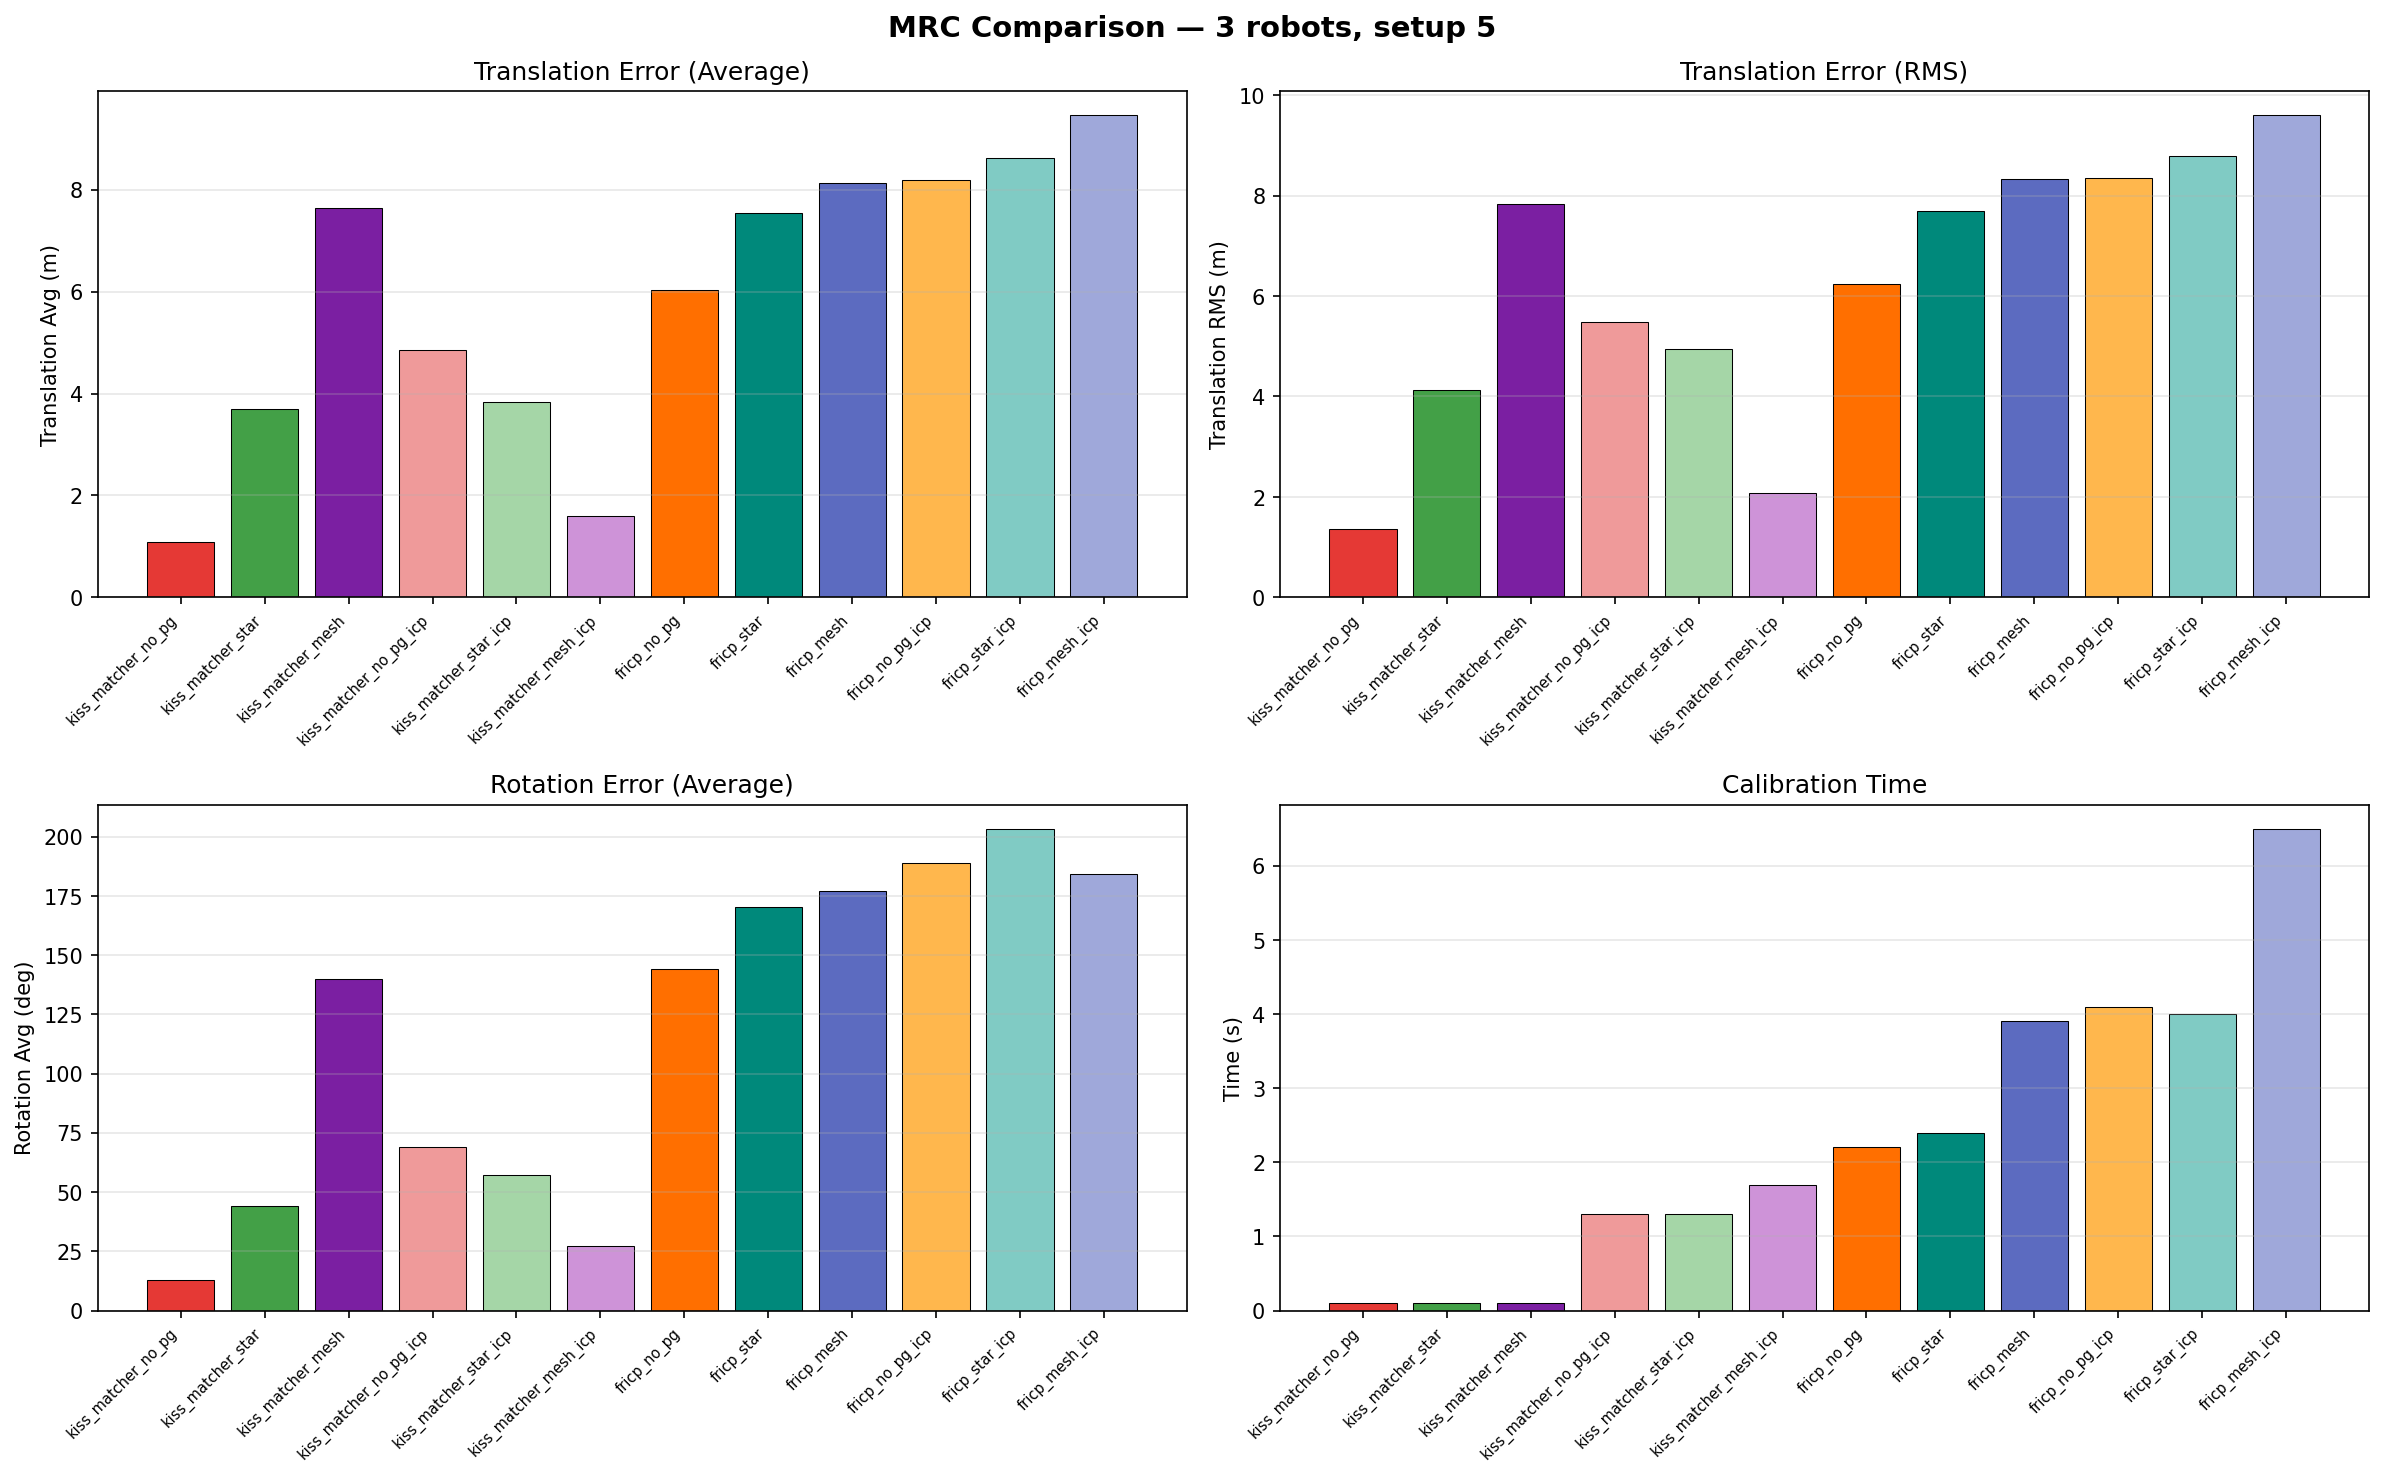
\includegraphics[width=0.95\textwidth]{figures/robots_3_setup_5_bars.png}
    \caption{Configuration comparison --- 3~robots, Setup~5.}
    \label{fig:app_3r_s5_bars}
\end{figure}

\begin{figure}[htbp]
    \centering
    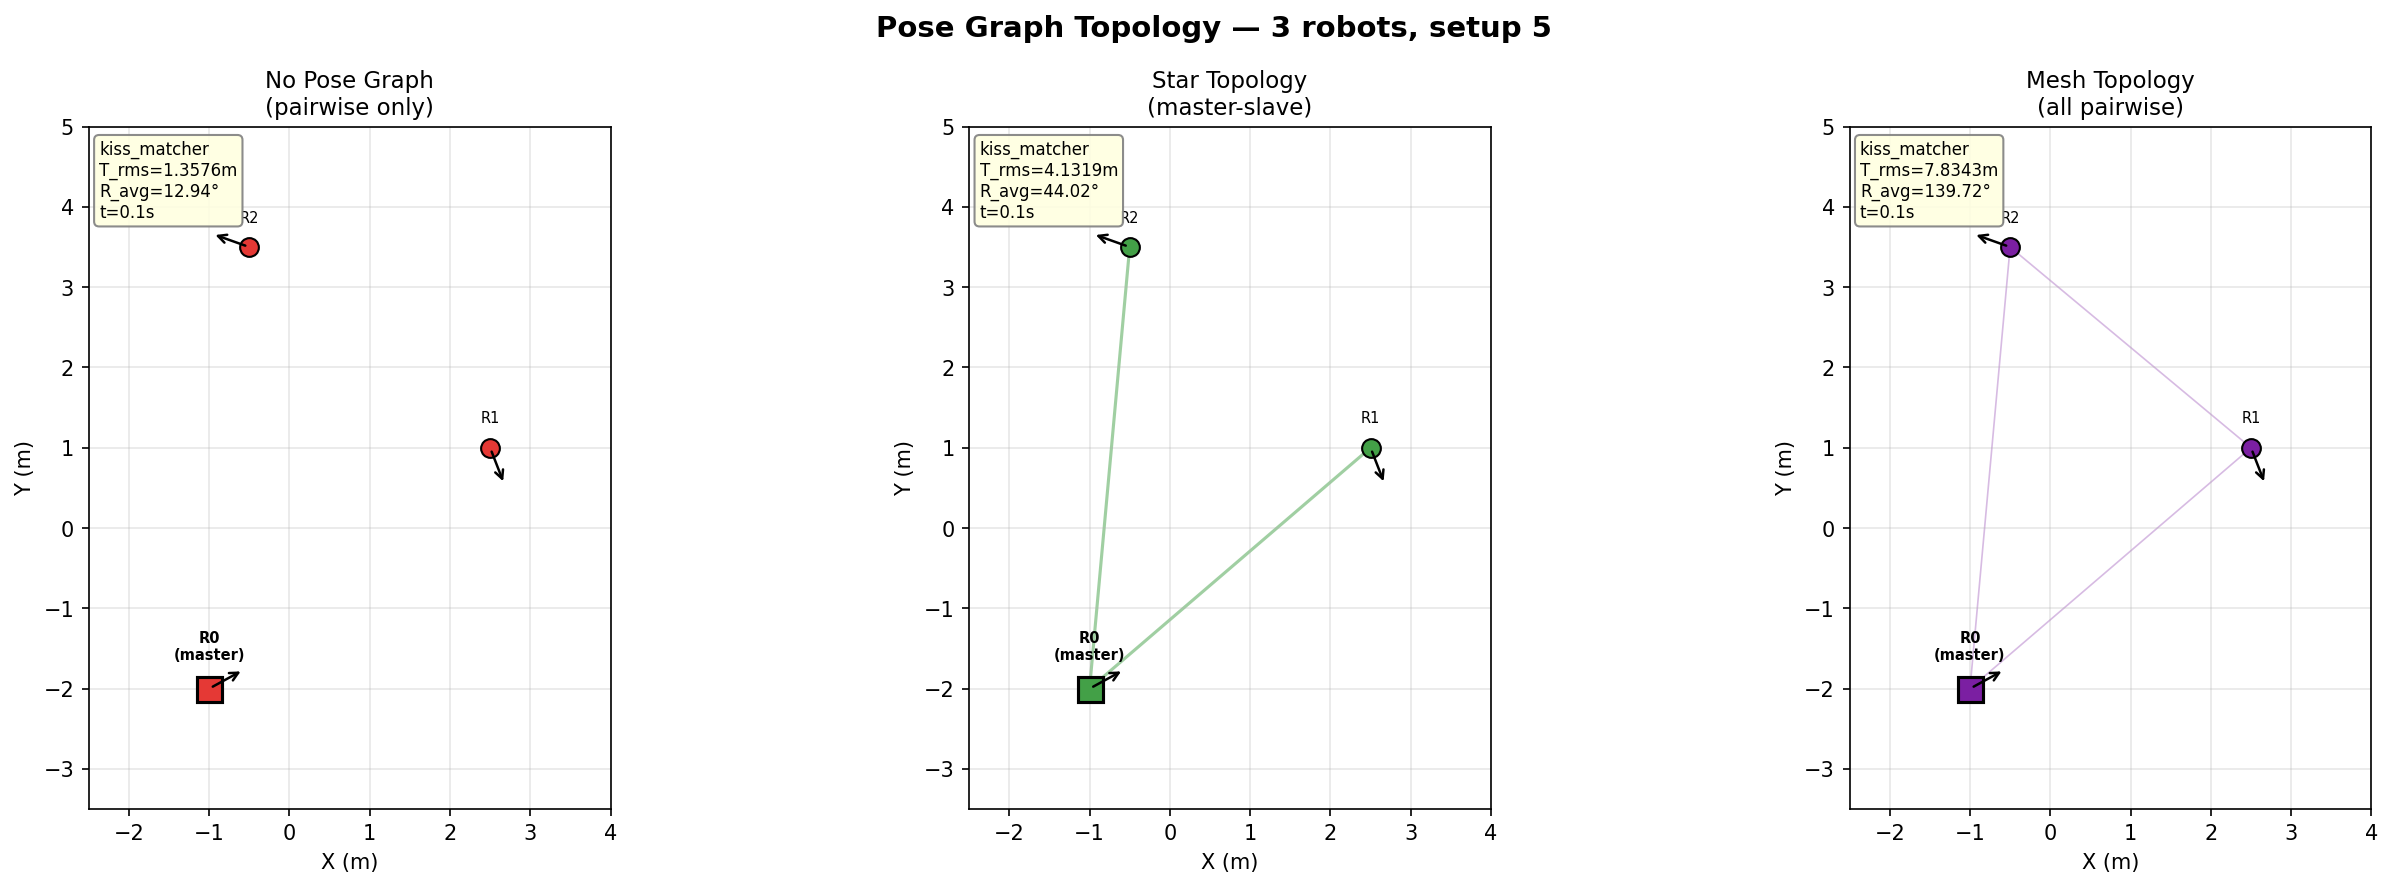
\includegraphics[width=0.7\textwidth]{figures/robots_3_setup_5_pose_graph.png}
    \caption{Pose graph visualization --- 3~robots, Setup~5.}
    \label{fig:app_3r_s5_pg}
\end{figure}

\begin{figure}[htbp]
    \centering
    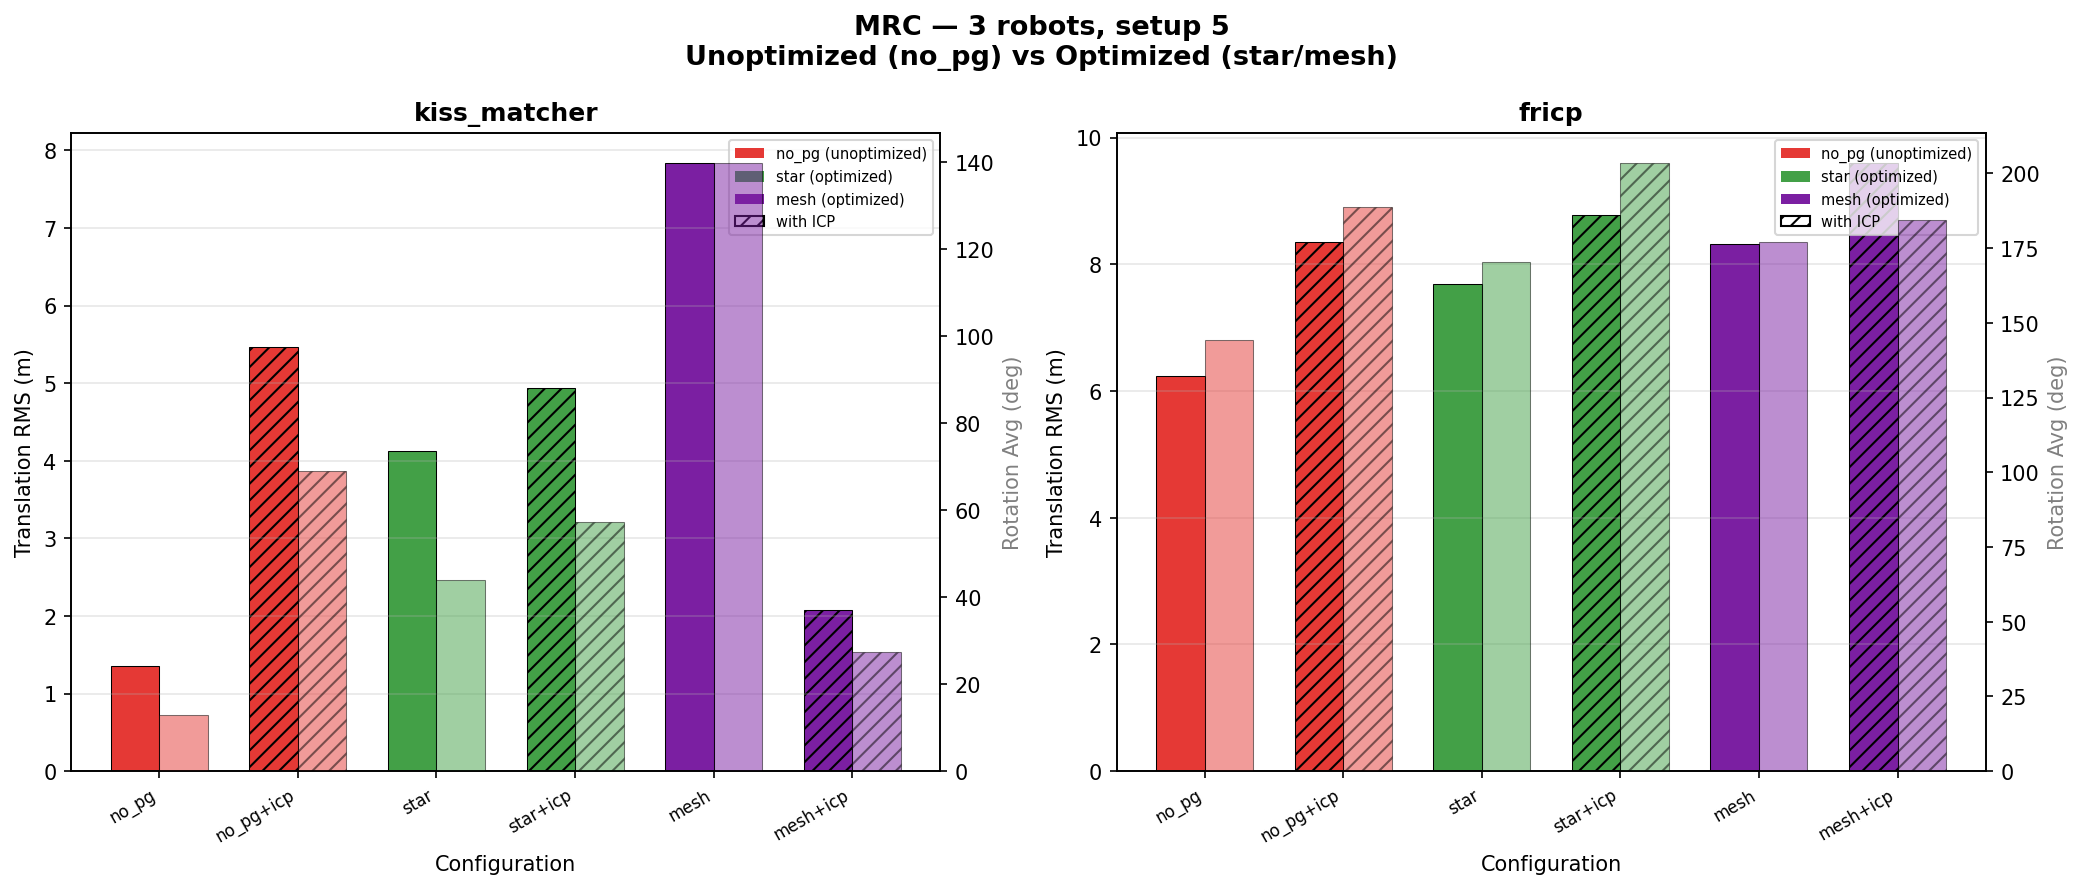
\includegraphics[width=0.95\textwidth]{figures/robots_3_setup_5_unopt_vs_opt.png}
    \caption{Unoptimized vs.\ optimized comparison --- 3~robots, Setup~5.}
    \label{fig:app_3r_s5_unopt}
\end{figure}

%% --- 3-robot averaged ---
\subsection{Averaged Results (3~Robots)}

\begin{table}[htbp]
    \centering
    \caption{3~robots --- averaged over all 5 position setups
             (3 trials per configuration).}
    \label{tab:app_3r_avg}
    \small
    \begin{tabular}{l r r r r r}
        \toprule
        \textbf{Configuration}
            & $\bar{e}_t$ [m]
            & $e_t^\mathrm{RMS}$ [m]
            & $\bar{e}_r$ [deg]
            & Ovlp [\%]
            & $t$ [s] \\
        \midrule
        \multicolumn{6}{l}{\textit{KISS-Matcher}} \\
        \quad no PG         & 2.97 & 3.44 &  49.5 & 58.6 & 0.1 \\
        \quad star PG       & 2.74 & 3.19 &  48.6 & 58.6 & 0.1 \\
        \quad mesh PG       & 2.55 & 2.85 &  44.6 & 58.6 & 0.1 \\
        \quad no PG + ICP   & \textbf{2.04} & \textbf{2.37} &  48.8 & 58.6 & 1.2 \\
        \quad star PG + ICP & 2.68 & 3.27 &  70.1 & 58.6 & 1.2 \\
        \quad mesh PG + ICP & 2.81 & 3.31 &  73.6 & 58.6 & 1.6 \\
        \midrule
        \multicolumn{6}{l}{\textit{FRICP}} \\
        \quad no PG         & 4.06 & 4.43 & 120.3 & 58.6 & 1.9 \\
        \quad star PG       & 4.42 & 4.75 & 133.1 & 58.6 & 1.9 \\
        \quad mesh PG       & 5.11 & 5.32 & 138.7 & 58.6 & 2.9 \\
        \quad no PG + ICP   & 4.71 & 5.09 & 142.5 & 58.6 & 3.3 \\
        \quad star PG + ICP & 4.55 & 5.02 & 136.0 & 58.6 & 3.3 \\
        \quad mesh PG + ICP & 5.23 & 5.69 & 135.7 & 58.6 & 5.2 \\
        \bottomrule
    \end{tabular}
\end{table}

\subsection{Cross-Setup Summary (3~Robots)}

\begin{figure}[htbp]
    \centering
    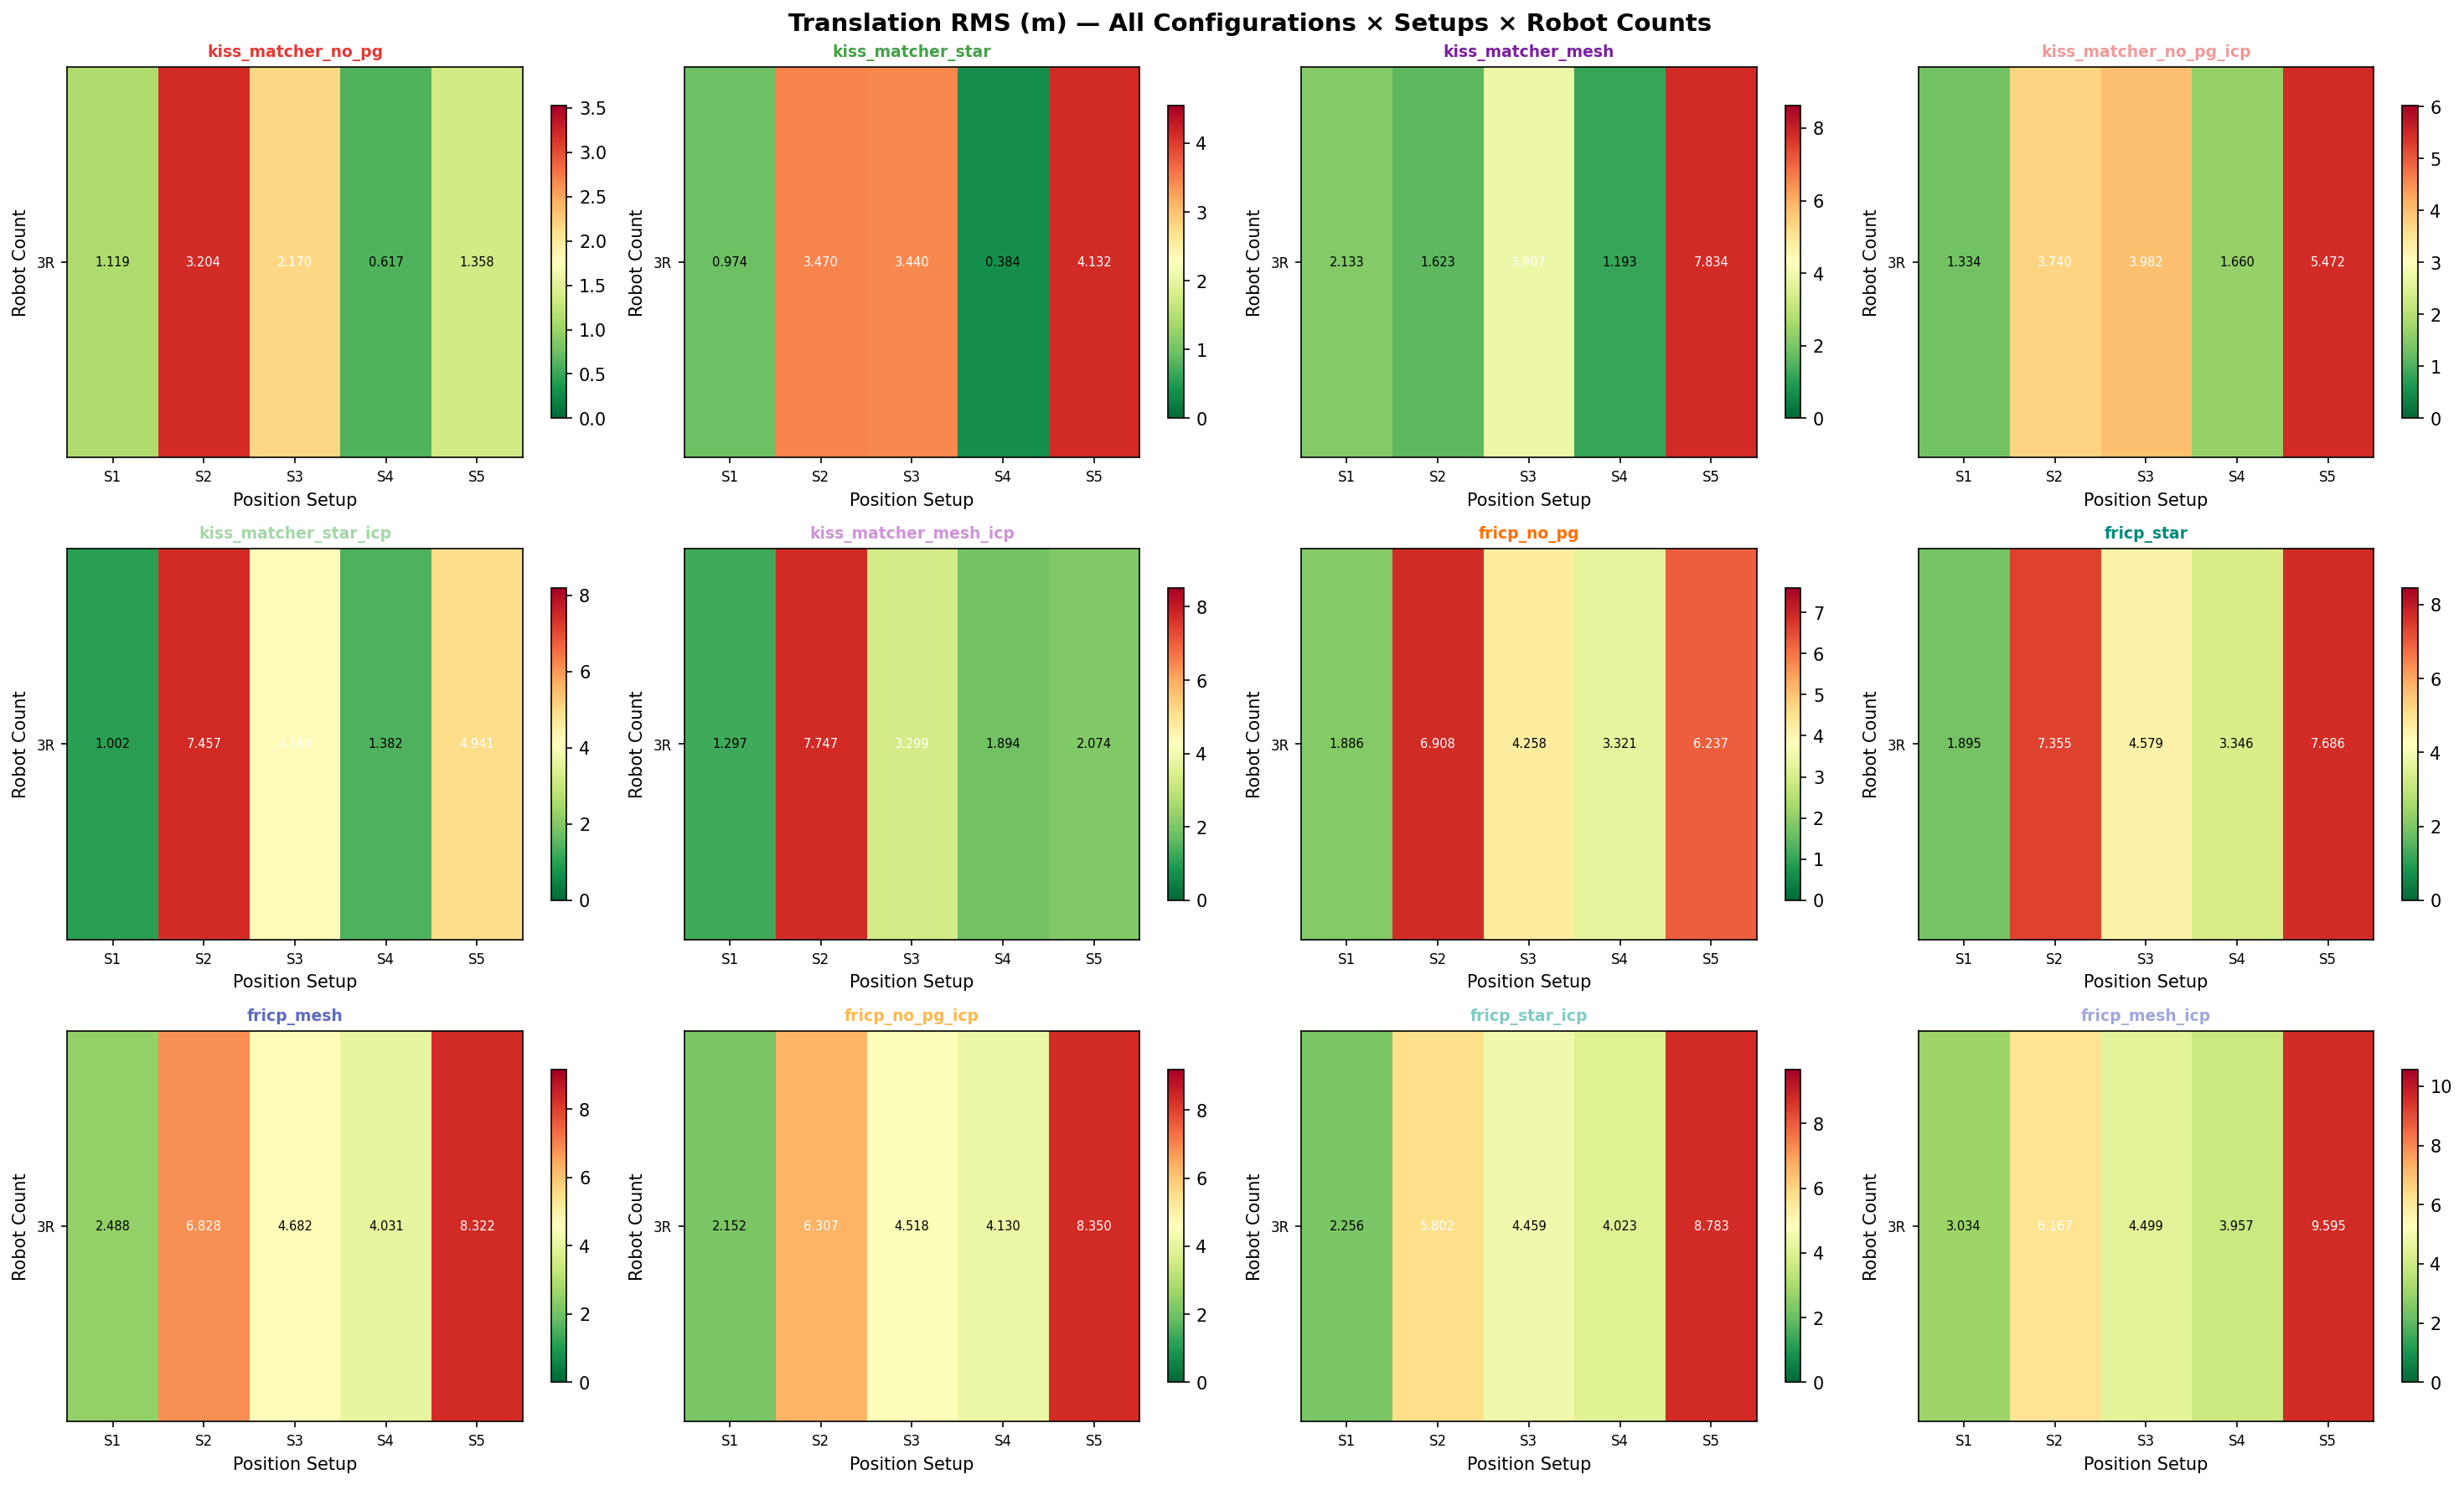
\includegraphics[width=\textwidth]{figures/heatmap_3_robots.png}
    \caption{Heatmap of translation RMS across position setups
             for all 12 configurations (3~robots).}
    \label{fig:app_3r_heatmap}
\end{figure}

\begin{figure}[htbp]
    \centering
    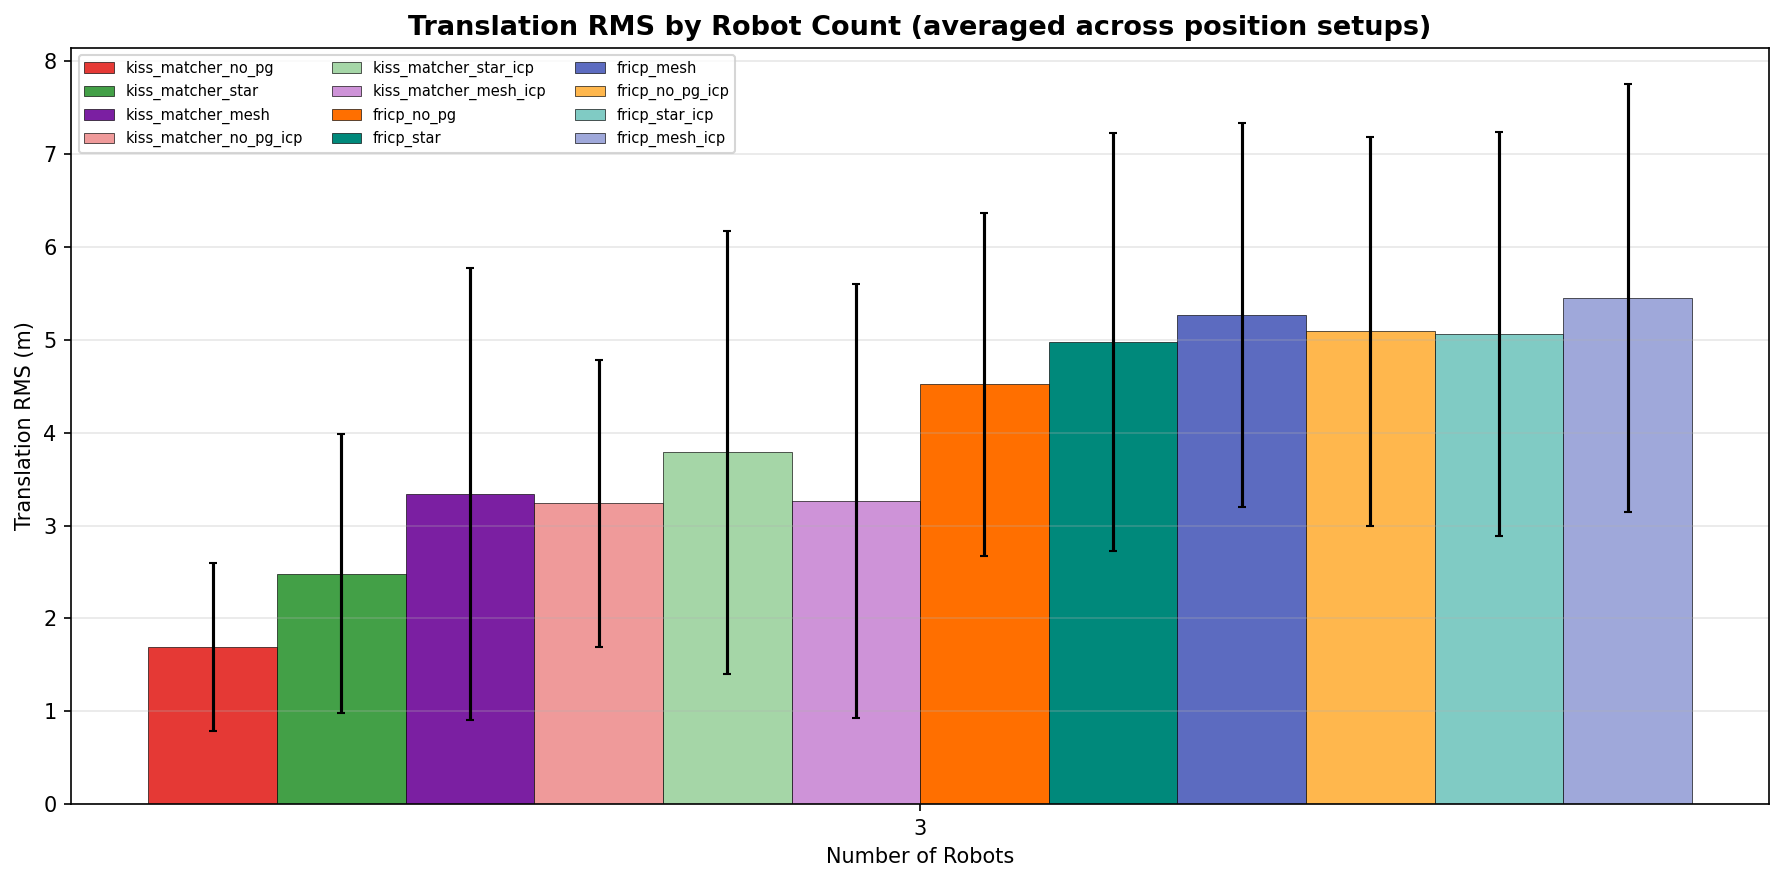
\includegraphics[width=\textwidth]{figures/summary_3_robots.png}
    \caption{Summary of translation RMS by configuration (3~robots).}
    \label{fig:app_3r_summary}
\end{figure}

%% ---------------------------------------------------------------------------
\section{5-Robot Scalability Tests}
\label{sec:app_5robots}

Five homogeneous EC~Swift robots were deployed in the scalability
test world ($20 \times 20$\,m room, reduced physics).

%% --- Setup 1 ---
\subsection{Setup~1: Regular Pentagon}

\begin{table}[htbp]
    \centering
    \caption{5~robots, Setup~1 --- regular pentagon
             ($r = \SI{2}{\metre}$, overlap: 55.3\%).}
    \label{tab:app_5r_s1}
    \small
    \begin{tabular}{l r r r r r}
        \toprule
        \textbf{Configuration}
            & $\bar{e}_t$ [m]
            & $e_t^\mathrm{RMS}$ [m]
            & $\bar{e}_r$ [deg]
            & Ovlp [\%]
            & $t$ [s] \\
        \midrule
        \multicolumn{6}{l}{\textit{KISS-Matcher}} \\
        \quad no PG         & 2.62 & 3.07 & 110.1 & 55.3 &  0.4 \\
        \quad star PG       & 1.65 & 2.04 &  58.2 & 55.3 &  0.5 \\
        \quad mesh PG       & 2.76 & 3.13 &  84.0 & 55.3 &  0.4 \\
        \quad no PG + ICP   & 2.83 & 3.66 & 105.0 & 55.3 &  2.8 \\
        \quad star PG + ICP & 2.26 & 2.92 &  64.8 & 55.3 &  3.1 \\
        \quad mesh PG + ICP & 1.42 & 1.98 &  41.7 & 55.3 &  6.3 \\
        \midrule
        \multicolumn{6}{l}{\textit{FRICP}} \\
        \quad no PG         & 3.78 & 4.03 & 143.0 & 55.3 &  3.6 \\
        \quad star PG       & 4.55 & 4.71 & 178.2 & 55.3 &  3.6 \\
        \quad mesh PG       & 4.77 & 4.92 & 171.9 & 55.3 & 10.9 \\
        \quad no PG + ICP   & 4.95 & 5.06 & 190.8 & 55.3 &  6.1 \\
        \quad star PG + ICP & 5.02 & 5.11 & 196.8 & 55.3 &  6.3 \\
        \quad mesh PG + ICP & 5.15 & 5.26 & 181.5 & 55.3 & 19.0 \\
        \bottomrule
    \end{tabular}
\end{table}

\begin{figure}[htbp]
    \centering
    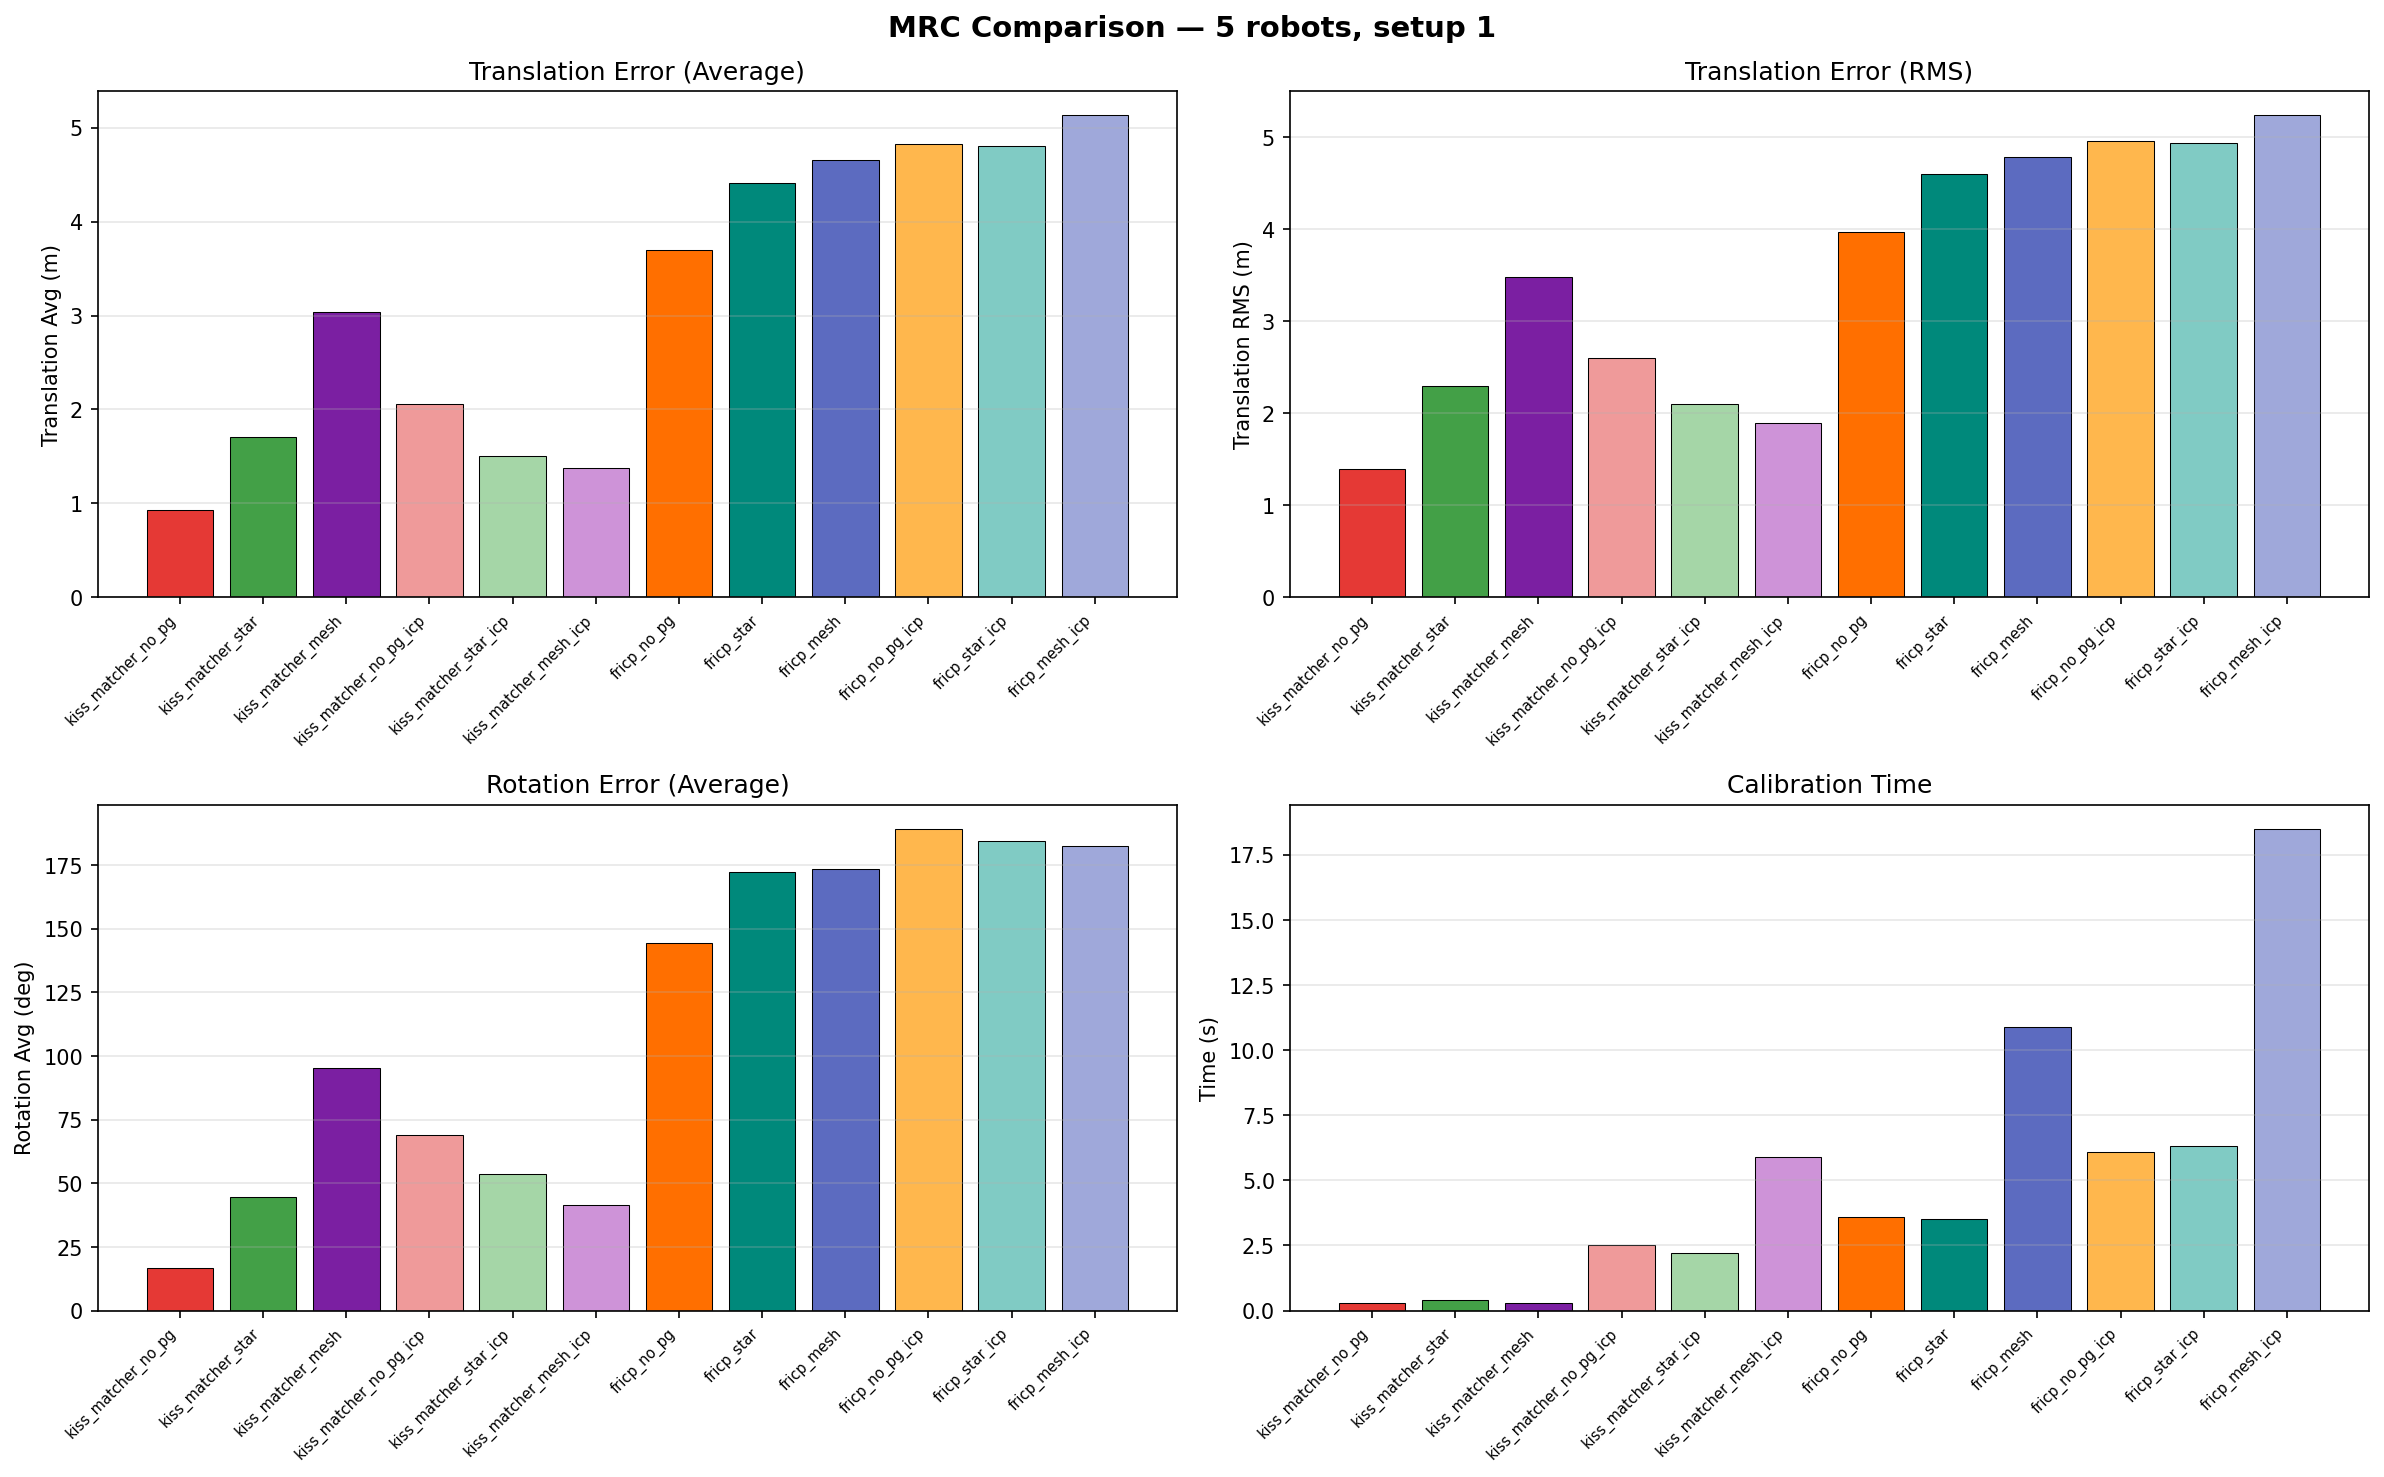
\includegraphics[width=0.95\textwidth]{figures/robots_5_setup_1_bars.png}
    \caption{Configuration comparison --- 5~robots, Setup~1.}
    \label{fig:app_5r_s1_bars}
\end{figure}

\begin{figure}[htbp]
    \centering
    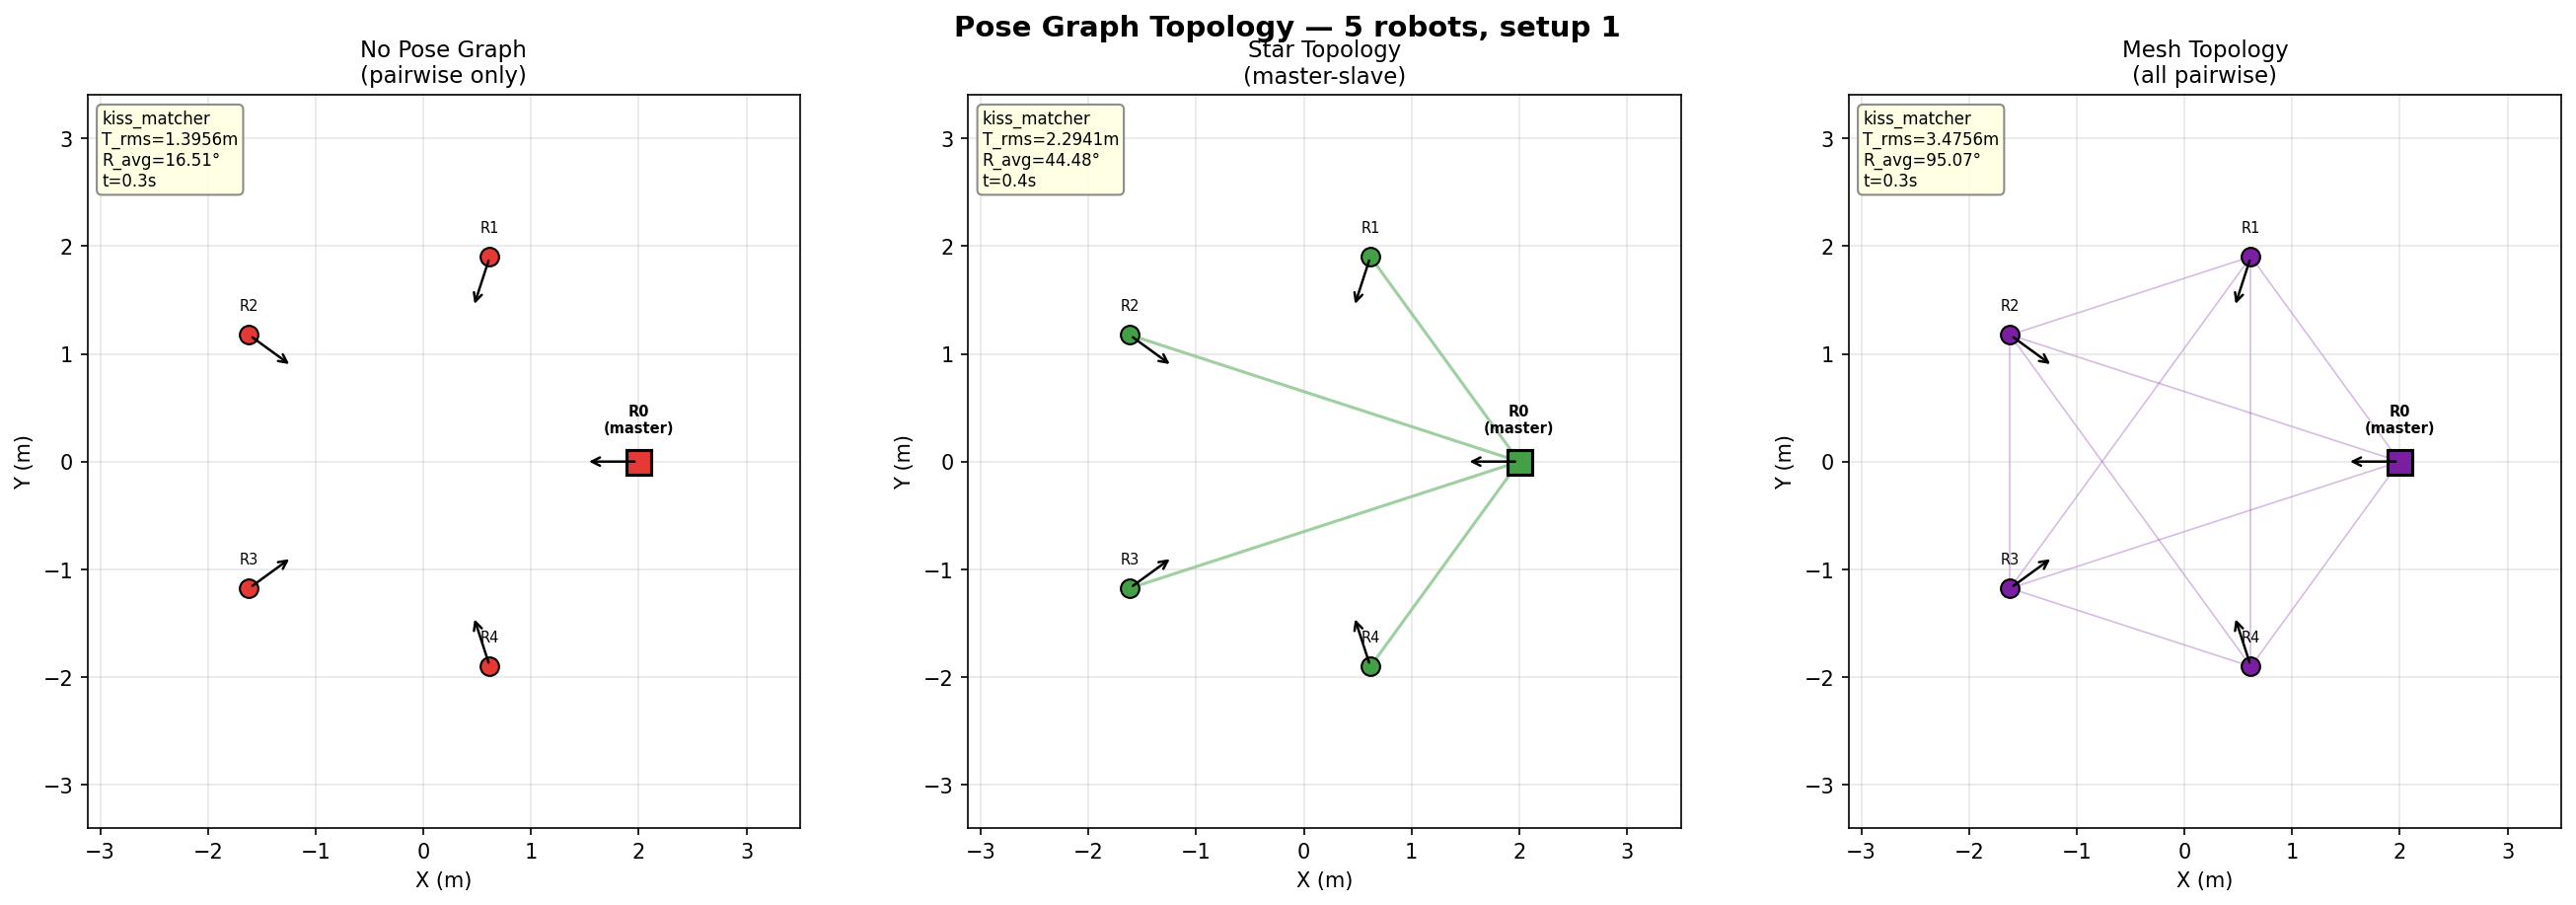
\includegraphics[width=0.7\textwidth]{figures/robots_5_setup_1_pose_graph.png}
    \caption{Pose graph visualization --- 5~robots, Setup~1.}
    \label{fig:app_5r_s1_pg}
\end{figure}

\begin{figure}[htbp]
    \centering
    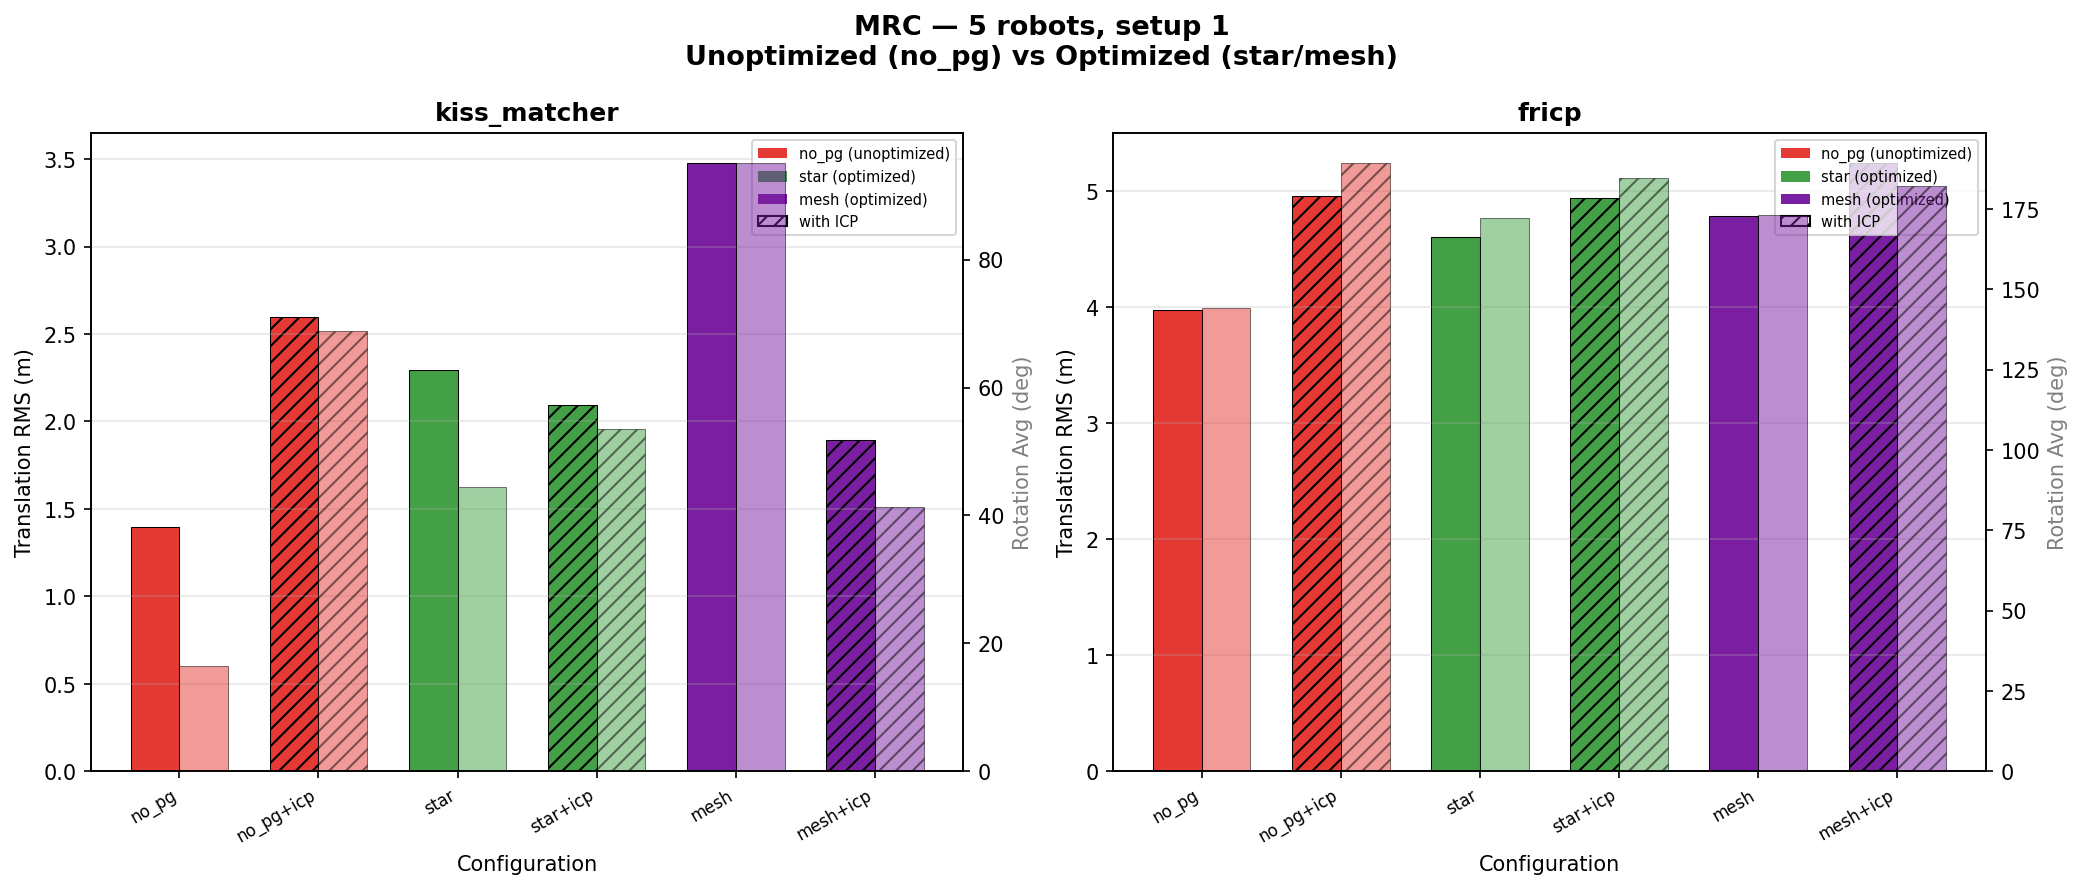
\includegraphics[width=0.95\textwidth]{figures/robots_5_setup_1_unopt_vs_opt.png}
    \caption{Unoptimized vs.\ optimized comparison --- 5~robots, Setup~1.}
    \label{fig:app_5r_s1_unopt}
\end{figure}

%% --- Setup 2 ---
\subsection{Setup~2: Wide Pentagon}

\begin{table}[htbp]
    \centering
    \caption{5~robots, Setup~2 --- wide pentagon
             (overlap: 17.1\%).}
    \label{tab:app_5r_s2}
    \small
    \begin{tabular}{l r r r r r}
        \toprule
        \textbf{Configuration}
            & $\bar{e}_t$ [m]
            & $e_t^\mathrm{RMS}$ [m]
            & $\bar{e}_r$ [deg]
            & Ovlp [\%]
            & $t$ [s] \\
        \midrule
        \multicolumn{6}{l}{\textit{KISS-Matcher}} \\
        \quad no PG         & 10.01 & 10.63 & 117.2 & 17.1 &  0.7 \\
        \quad star PG       & 11.70 & 12.79 & 163.6 & 17.1 &  0.6 \\
        \quad mesh PG       & 13.29 & 14.48 & 173.5 & 17.1 &  0.7 \\
        \quad no PG + ICP   & 13.09 & 14.32 & 182.8 & 17.1 &  2.3 \\
        \quad star PG + ICP & 13.34 & 14.39 & 153.2 & 17.1 &  3.0 \\
        \quad mesh PG + ICP & 13.57 & 14.45 & 182.5 & 17.1 &  5.7 \\
        \midrule
        \multicolumn{6}{l}{\textit{FRICP}} \\
        \quad no PG         & 11.18 & 12.32 & 189.3 & 17.1 &  5.0 \\
        \quad star PG       & 10.93 & 11.99 & 181.1 & 17.1 &  5.0 \\
        \quad mesh PG       & 11.09 & 11.88 & 168.8 & 17.1 & 14.4 \\
        \quad no PG + ICP   & 11.07 & 11.93 & 176.6 & 17.1 &  8.2 \\
        \quad star PG + ICP & 10.81 & 11.86 & 173.1 & 17.1 &  8.7 \\
        \quad mesh PG + ICP & 10.91 & 11.79 & 170.8 & 17.1 & 23.0 \\
        \bottomrule
    \end{tabular}
\end{table}

\begin{figure}[htbp]
    \centering
    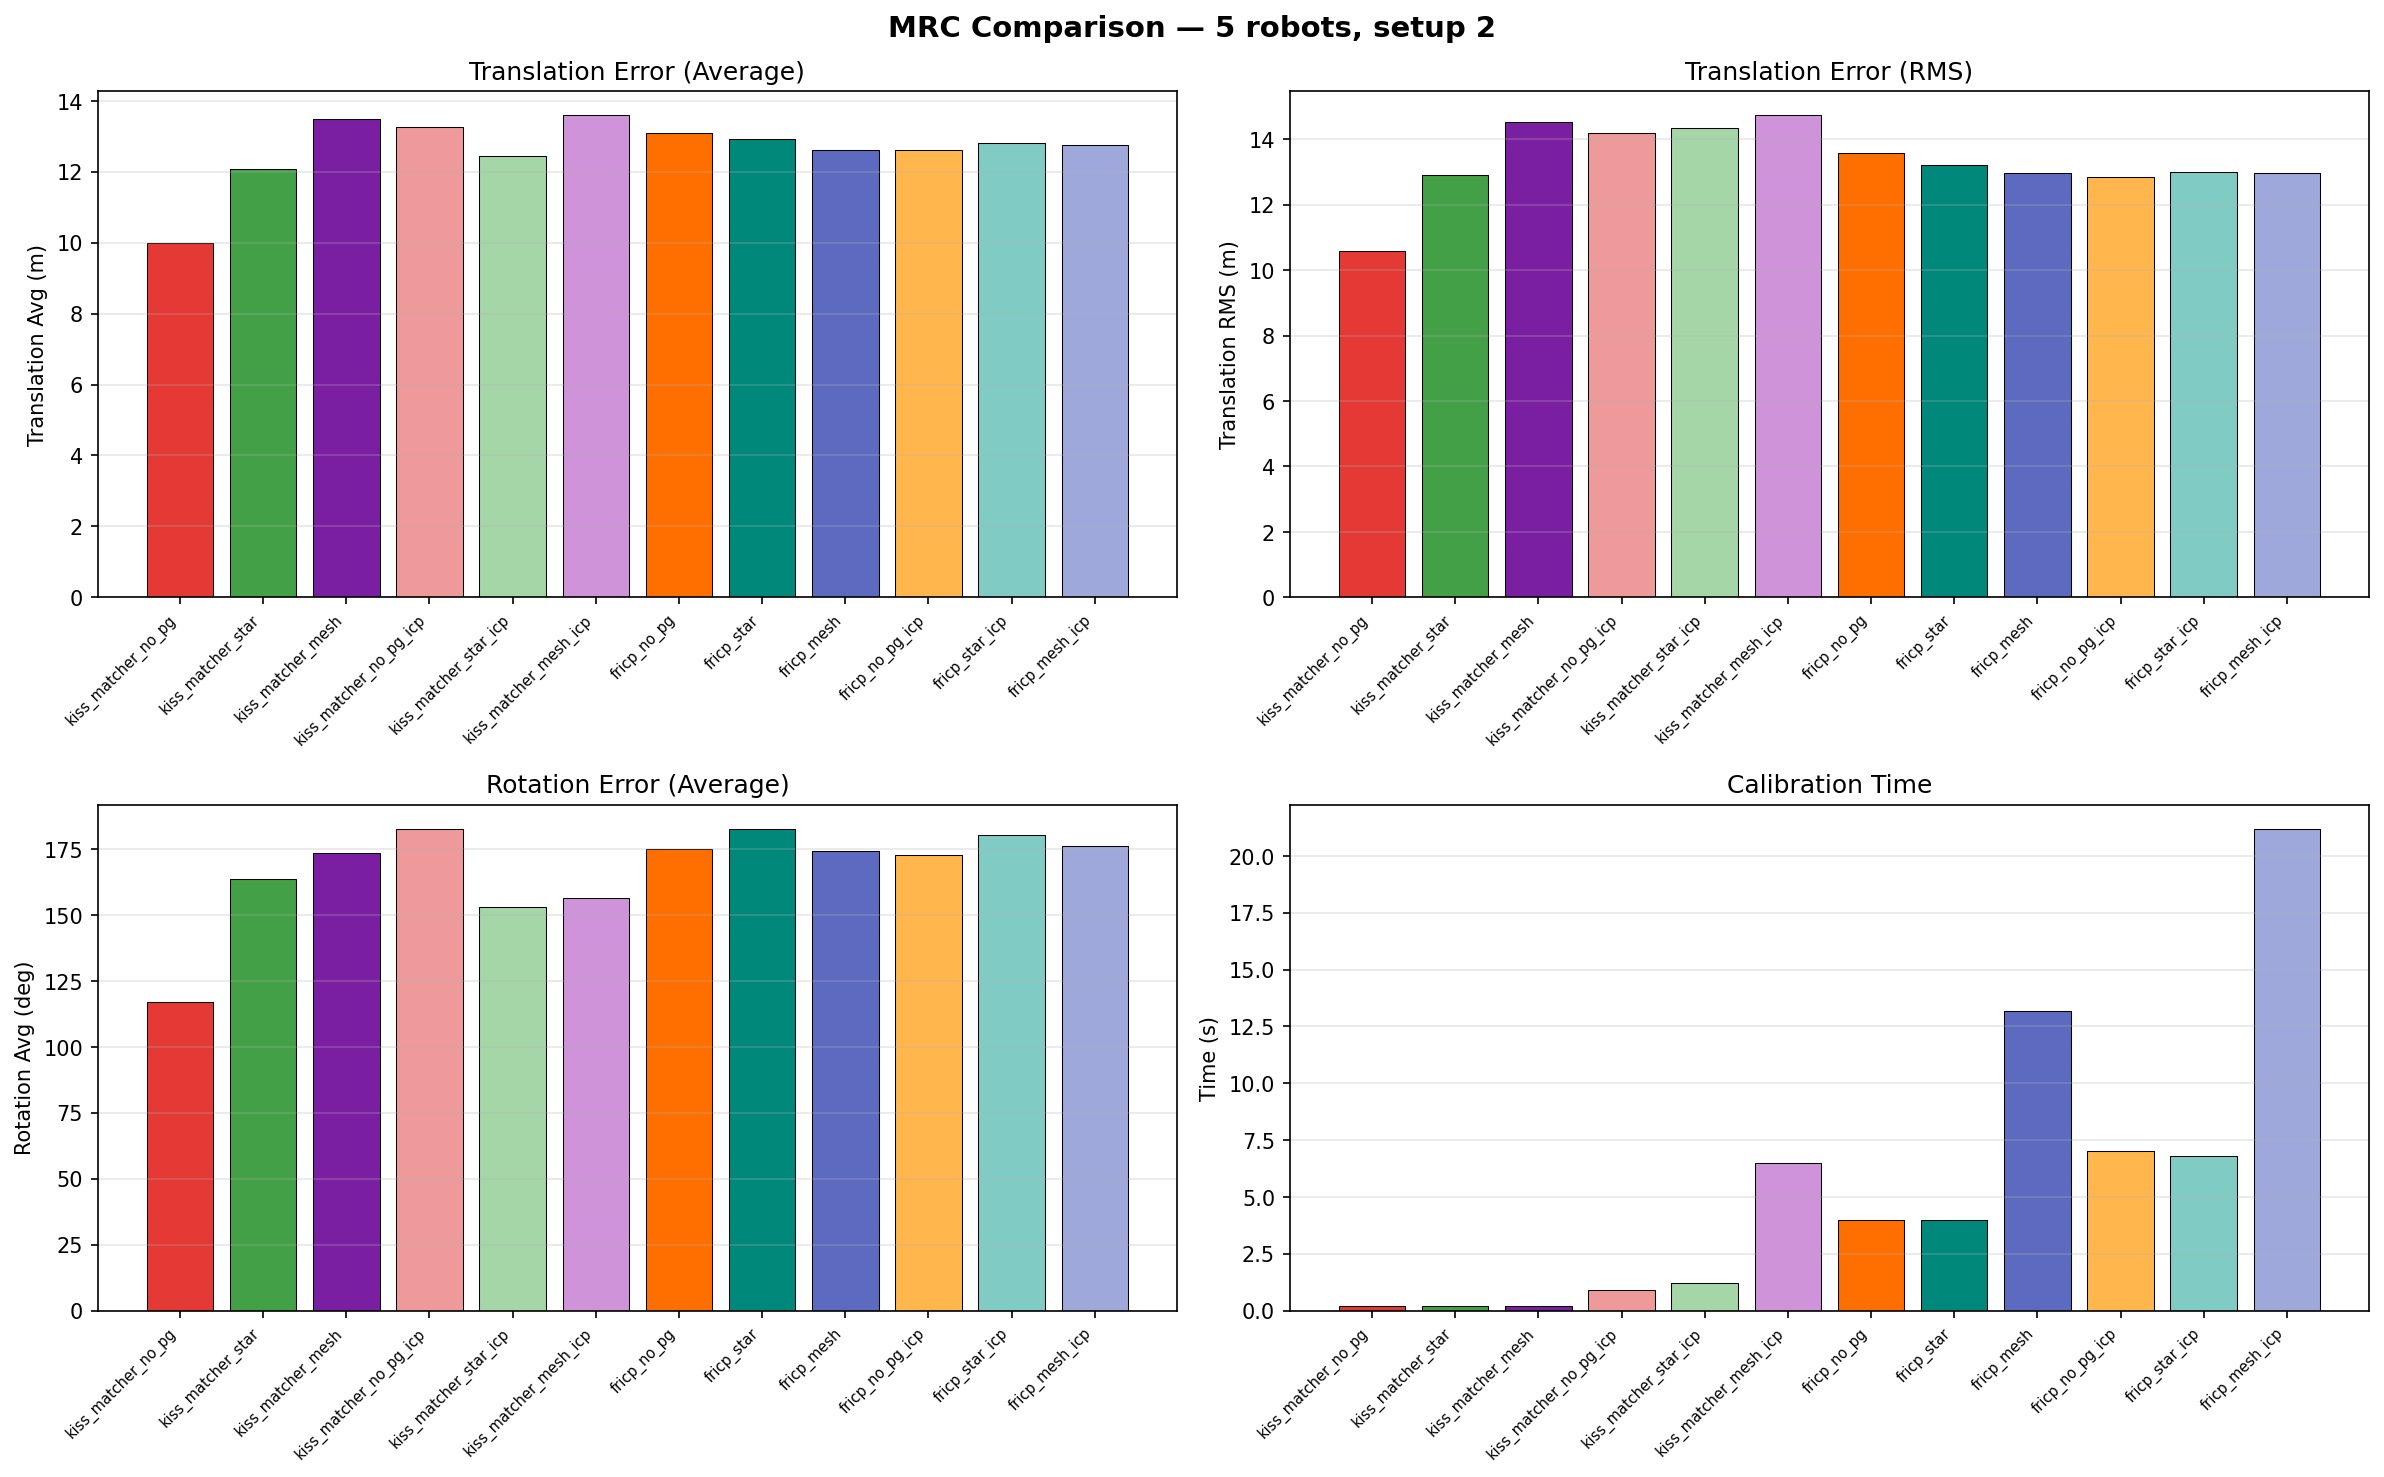
\includegraphics[width=0.95\textwidth]{figures/robots_5_setup_2_bars.png}
    \caption{Configuration comparison --- 5~robots, Setup~2.}
    \label{fig:app_5r_s2_bars}
\end{figure}

\begin{figure}[htbp]
    \centering
    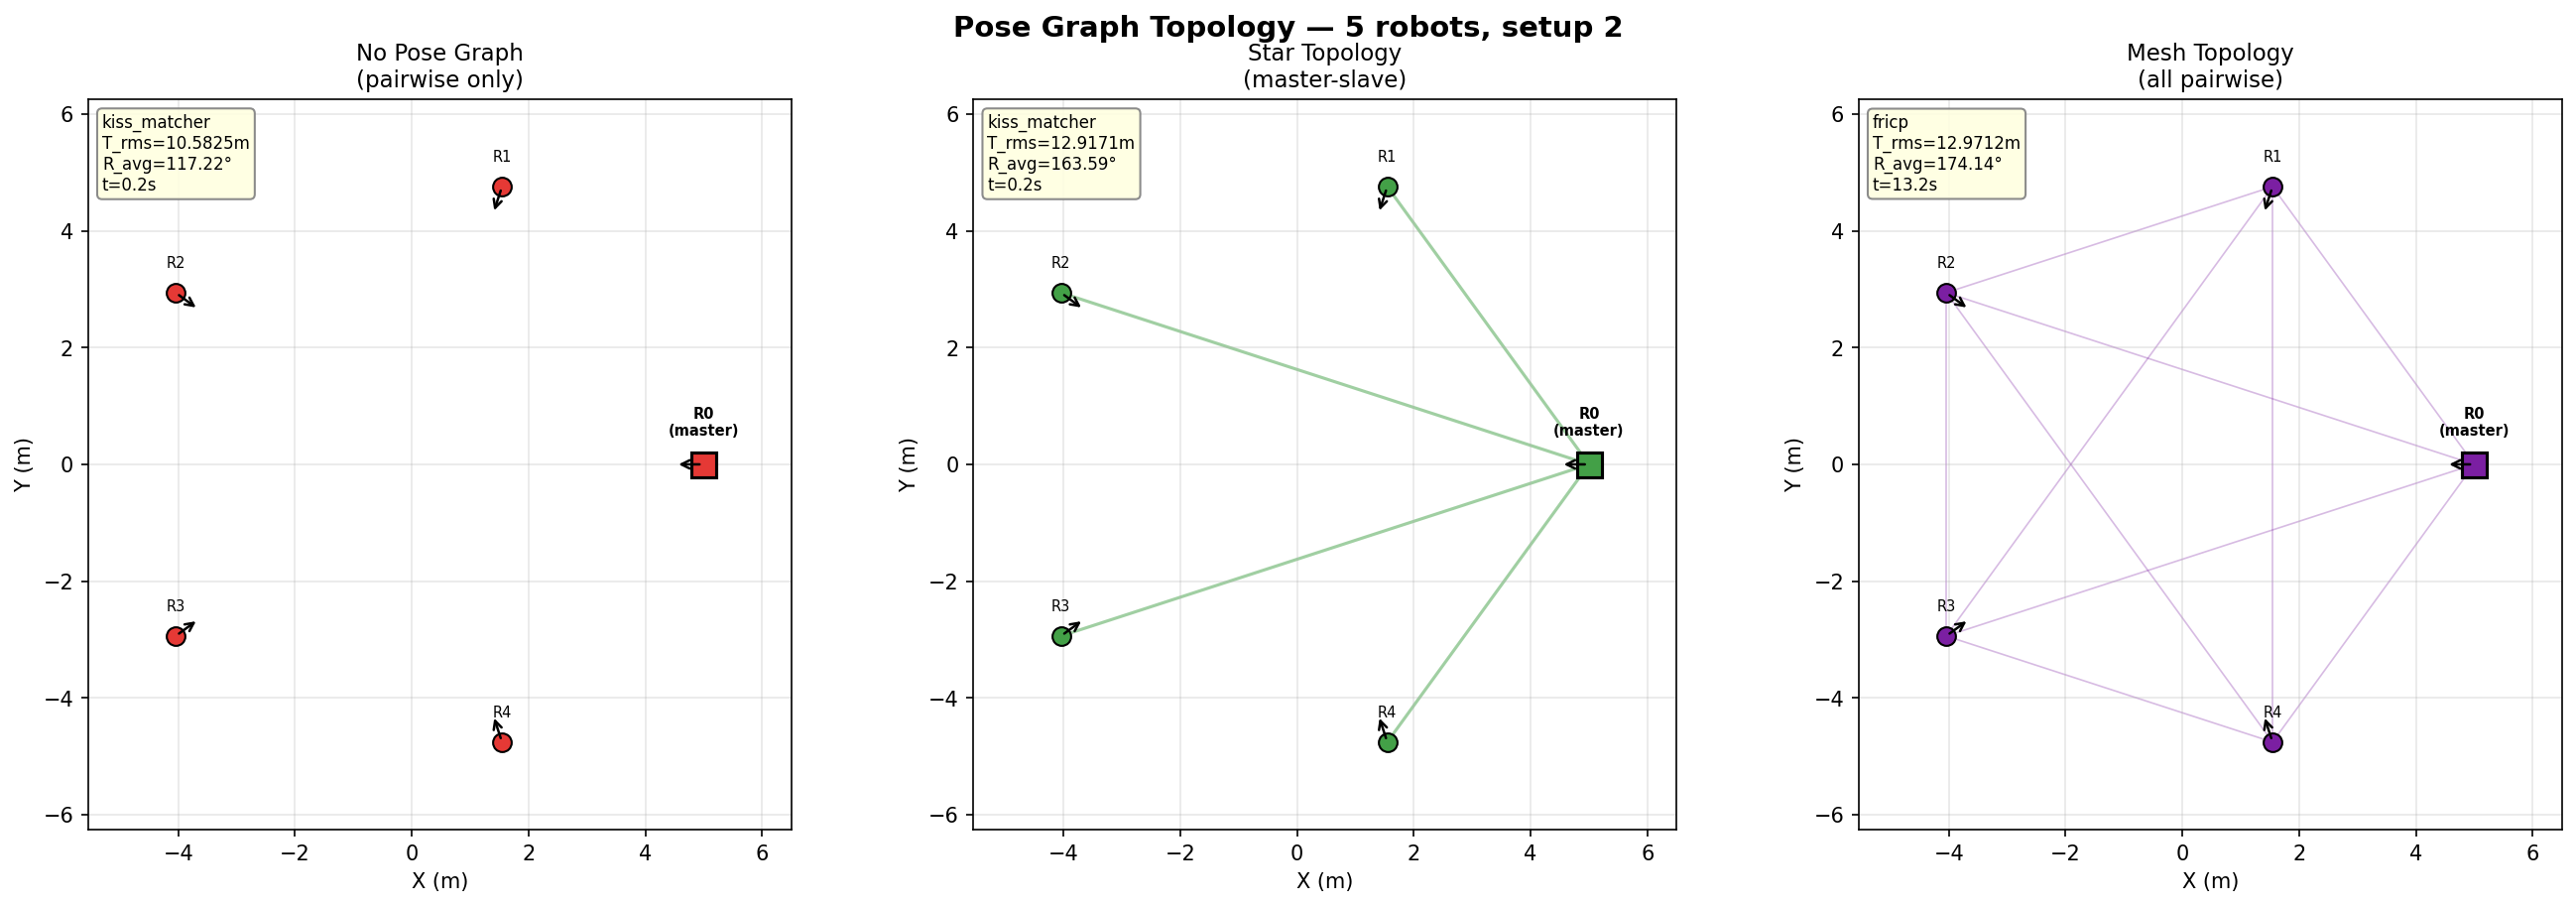
\includegraphics[width=0.7\textwidth]{figures/robots_5_setup_2_pose_graph.png}
    \caption{Pose graph visualization --- 5~robots, Setup~2.}
    \label{fig:app_5r_s2_pg}
\end{figure}

\begin{figure}[htbp]
    \centering
    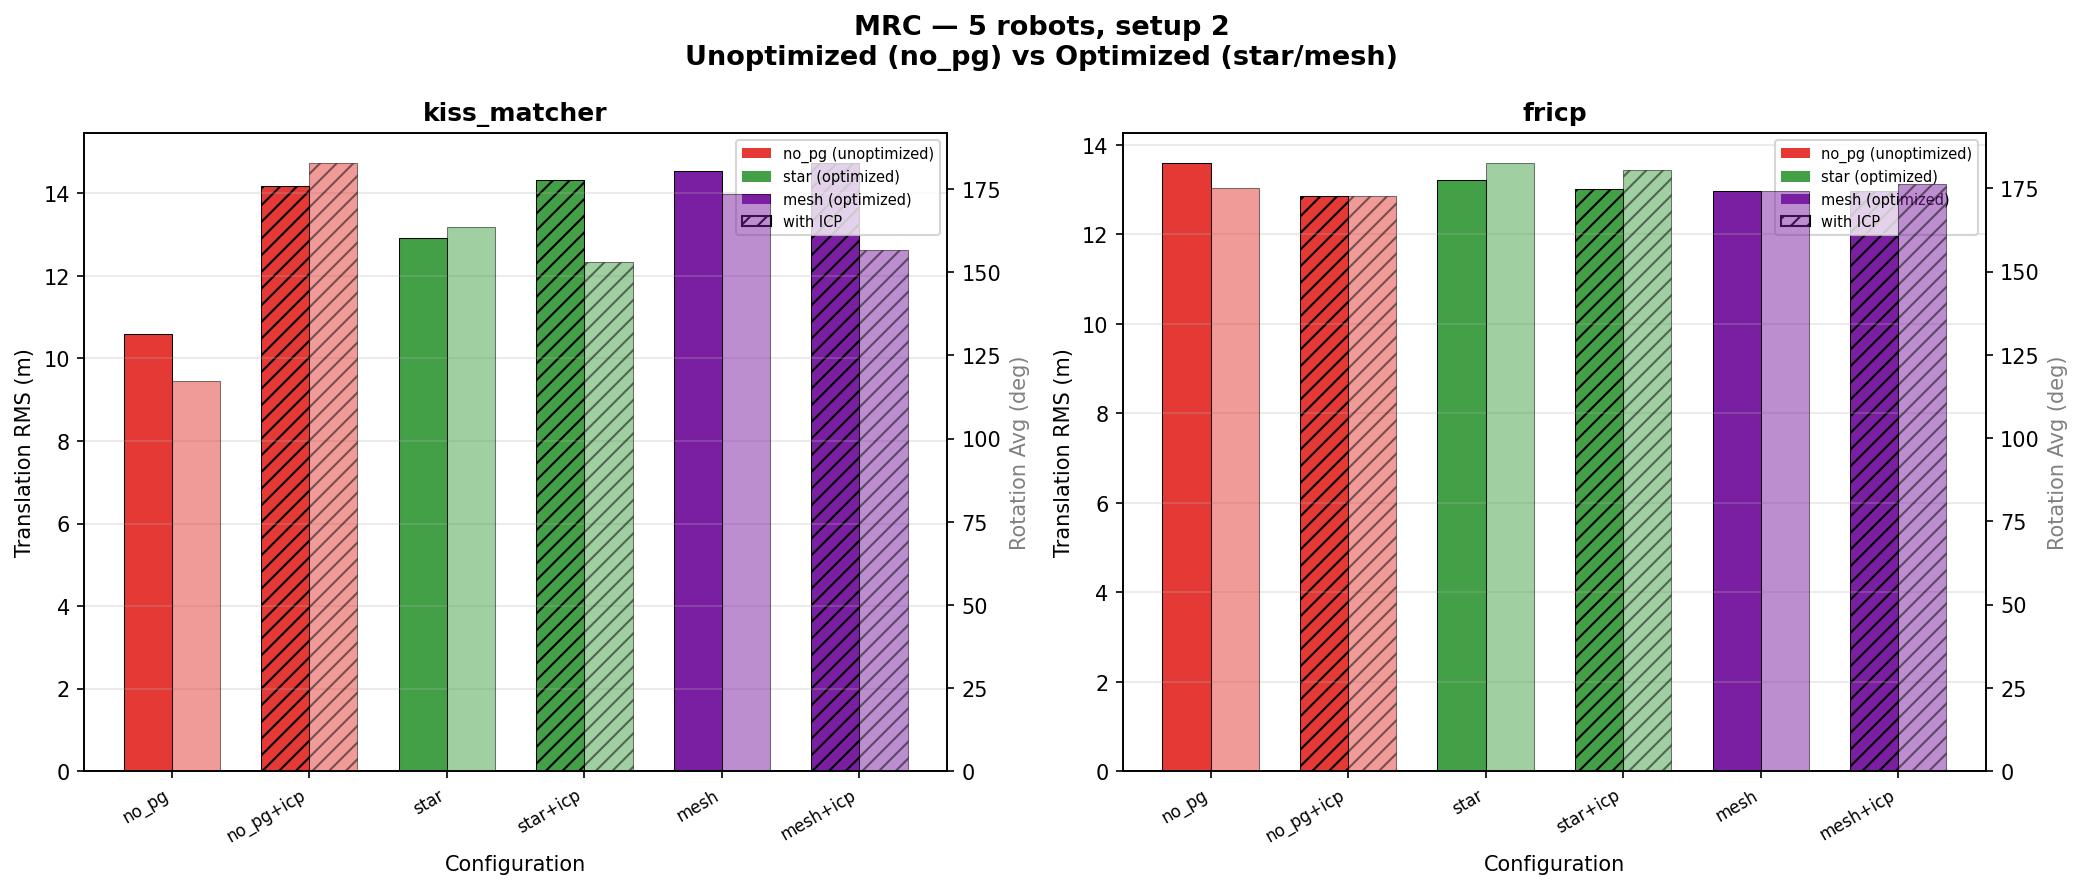
\includegraphics[width=0.95\textwidth]{figures/robots_5_setup_2_unopt_vs_opt.png}
    \caption{Unoptimized vs.\ optimized comparison --- 5~robots, Setup~2.}
    \label{fig:app_5r_s2_unopt}
\end{figure}

%% --- Setup 3 ---
\subsection{Setup~3: Grid Formation}

\begin{table}[htbp]
    \centering
    \caption{5~robots, Setup~3 --- grid formation
             (overlap: 59.2\%).}
    \label{tab:app_5r_s3}
    \small
    \begin{tabular}{l r r r r r}
        \toprule
        \textbf{Configuration}
            & $\bar{e}_t$ [m]
            & $e_t^\mathrm{RMS}$ [m]
            & $\bar{e}_r$ [deg]
            & Ovlp [\%]
            & $t$ [s] \\
        \midrule
        \multicolumn{6}{l}{\textit{KISS-Matcher}} \\
        \quad no PG         & 1.61 & 3.01 &  45.9 & 59.2 &  0.1 \\
        \quad star PG       & 2.24 & 3.98 &  62.8 & 59.2 &  0.1 \\
        \quad mesh PG       & 1.85 & 2.83 &  53.5 & 59.2 &  0.2 \\
        \quad no PG + ICP   & 2.00 & 3.67 &  55.4 & 59.2 &  3.0 \\
        \quad star PG + ICP & 2.18 & 4.20 &  63.5 & 59.2 &  2.9 \\
        \quad mesh PG + ICP & 1.25 & 2.29 &  35.3 & 59.2 &  6.2 \\
        \midrule
        \multicolumn{6}{l}{\textit{FRICP}} \\
        \quad no PG         & 3.73 & 4.47 & 101.8 & 59.2 &  3.2 \\
        \quad star PG       & 4.60 & 5.23 & 124.1 & 59.2 &  3.1 \\
        \quad mesh PG       & 4.98 & 5.59 & 131.4 & 59.2 &  7.9 \\
        \quad no PG + ICP   & 4.57 & 5.47 & 133.8 & 59.2 &  6.6 \\
        \quad star PG + ICP & 4.41 & 5.40 & 134.8 & 59.2 &  6.6 \\
        \quad mesh PG + ICP & 3.95 & 5.18 & 134.7 & 59.2 & 15.8 \\
        \bottomrule
    \end{tabular}
\end{table}

\begin{figure}[htbp]
    \centering
    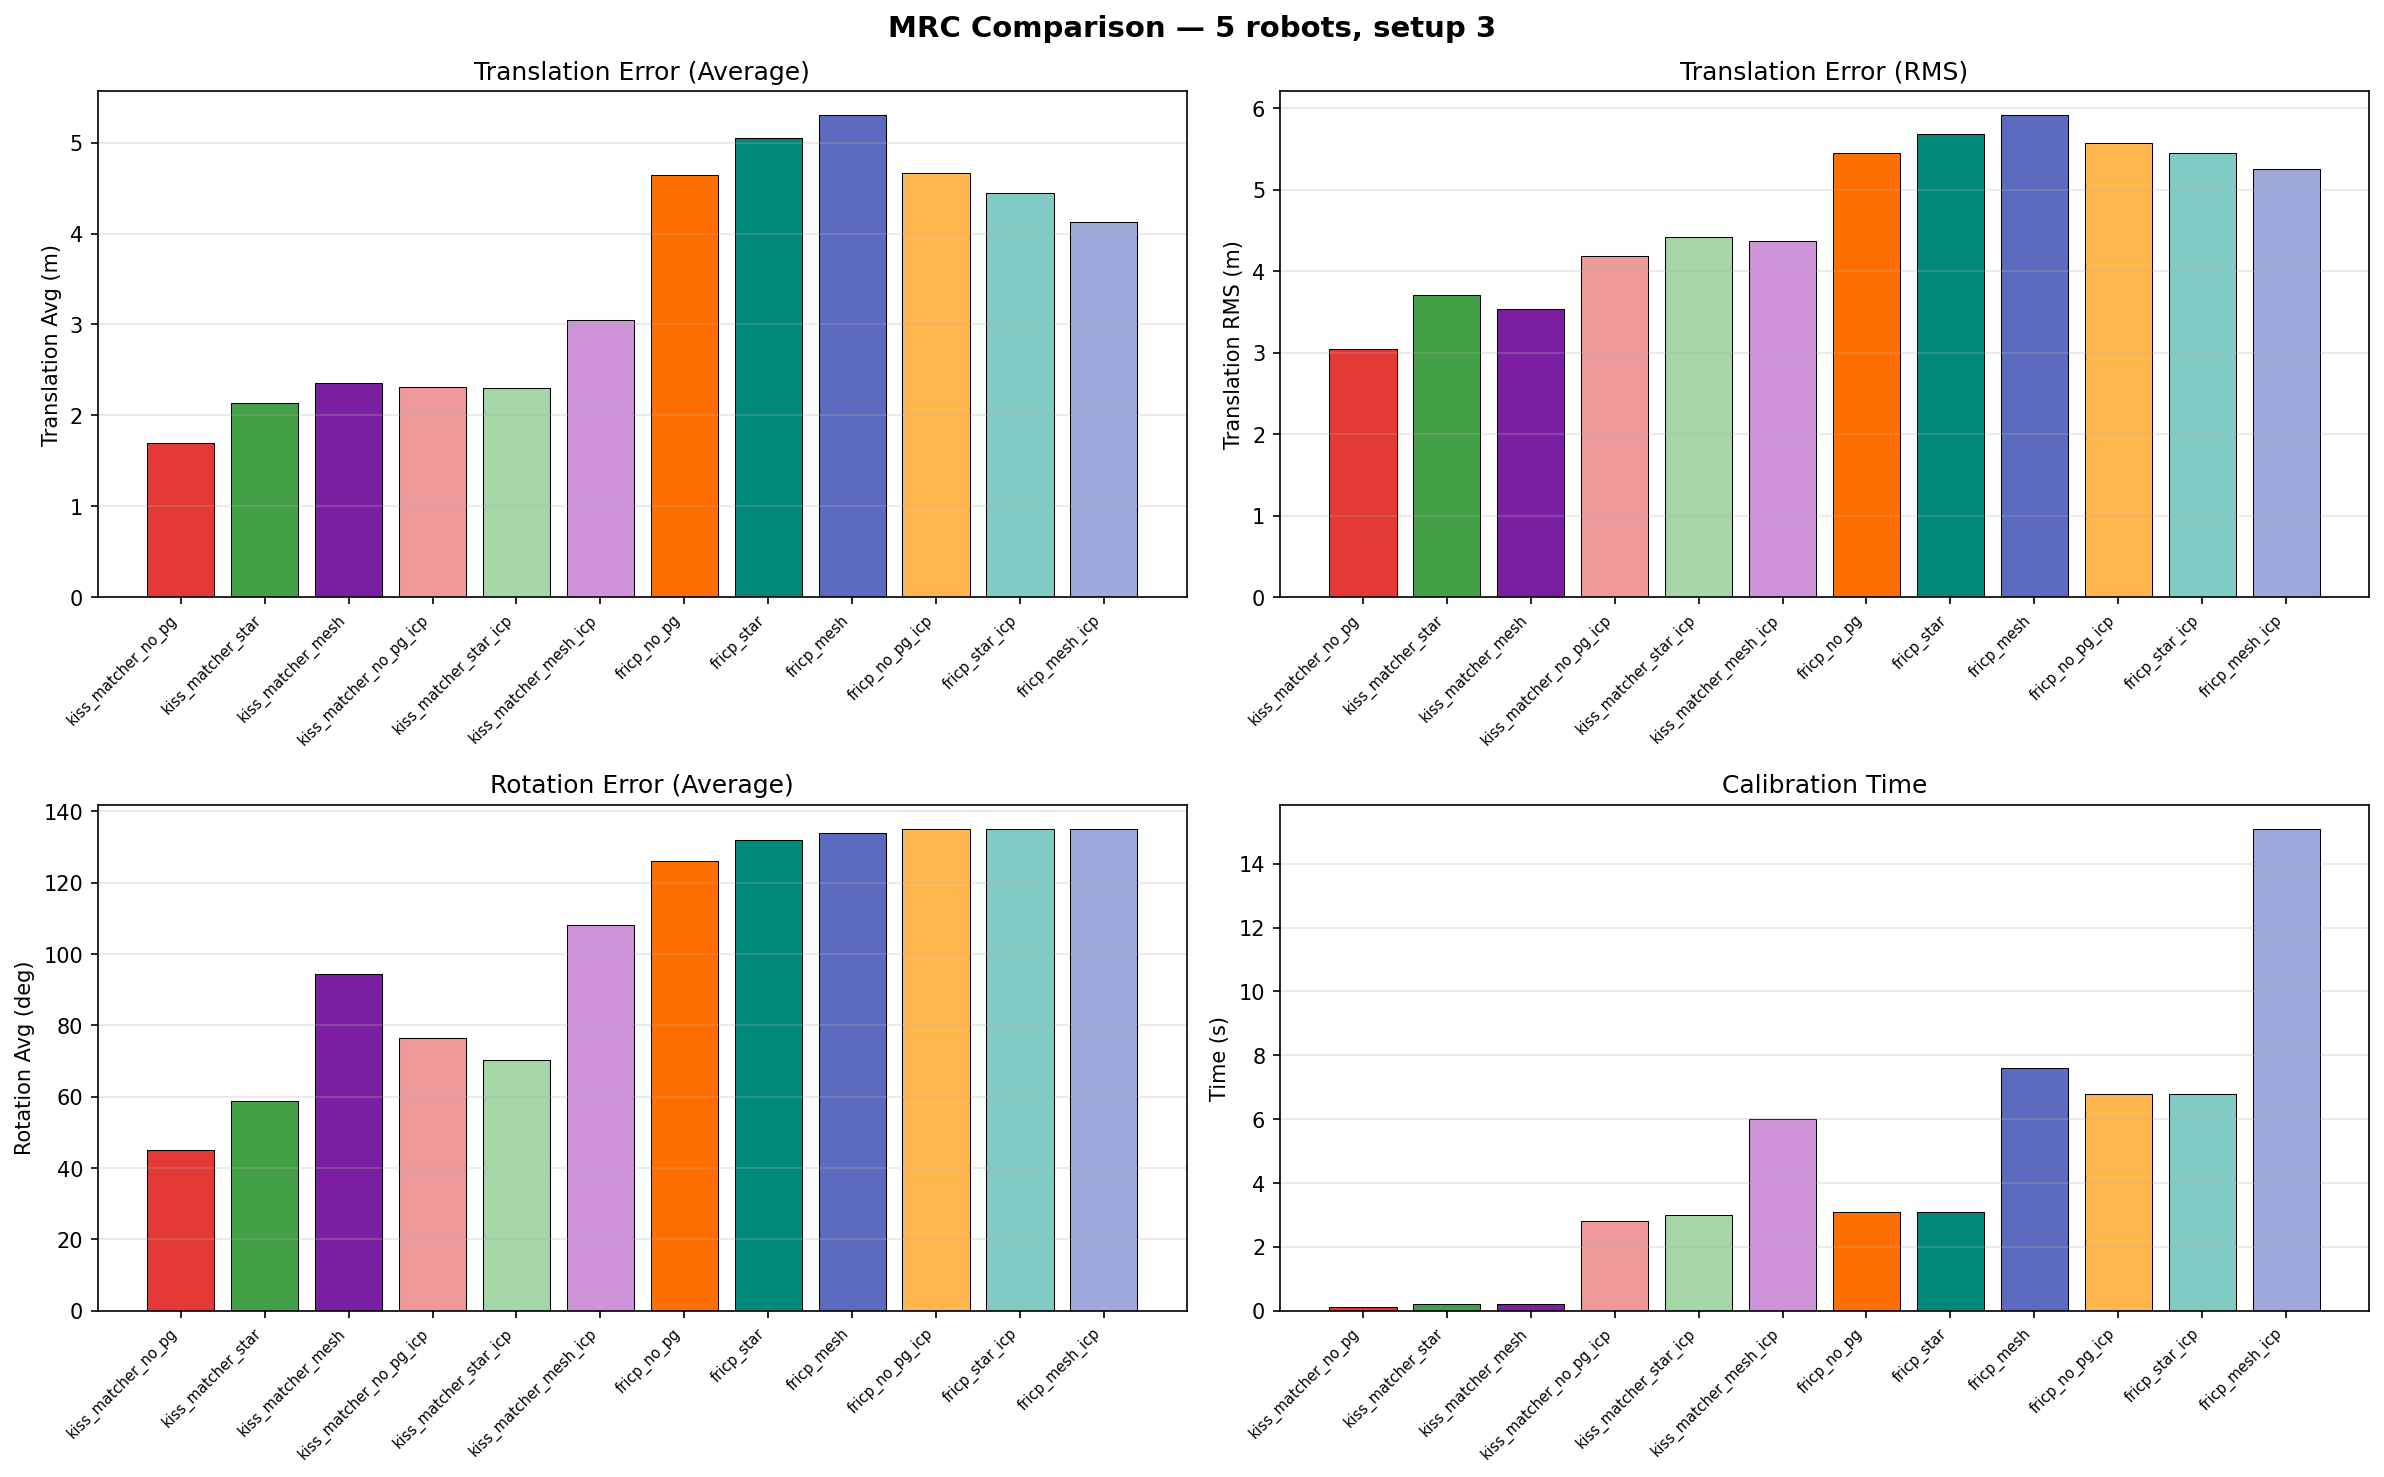
\includegraphics[width=0.95\textwidth]{figures/robots_5_setup_3_bars.png}
    \caption{Configuration comparison --- 5~robots, Setup~3.}
    \label{fig:app_5r_s3_bars}
\end{figure}

\begin{figure}[htbp]
    \centering
    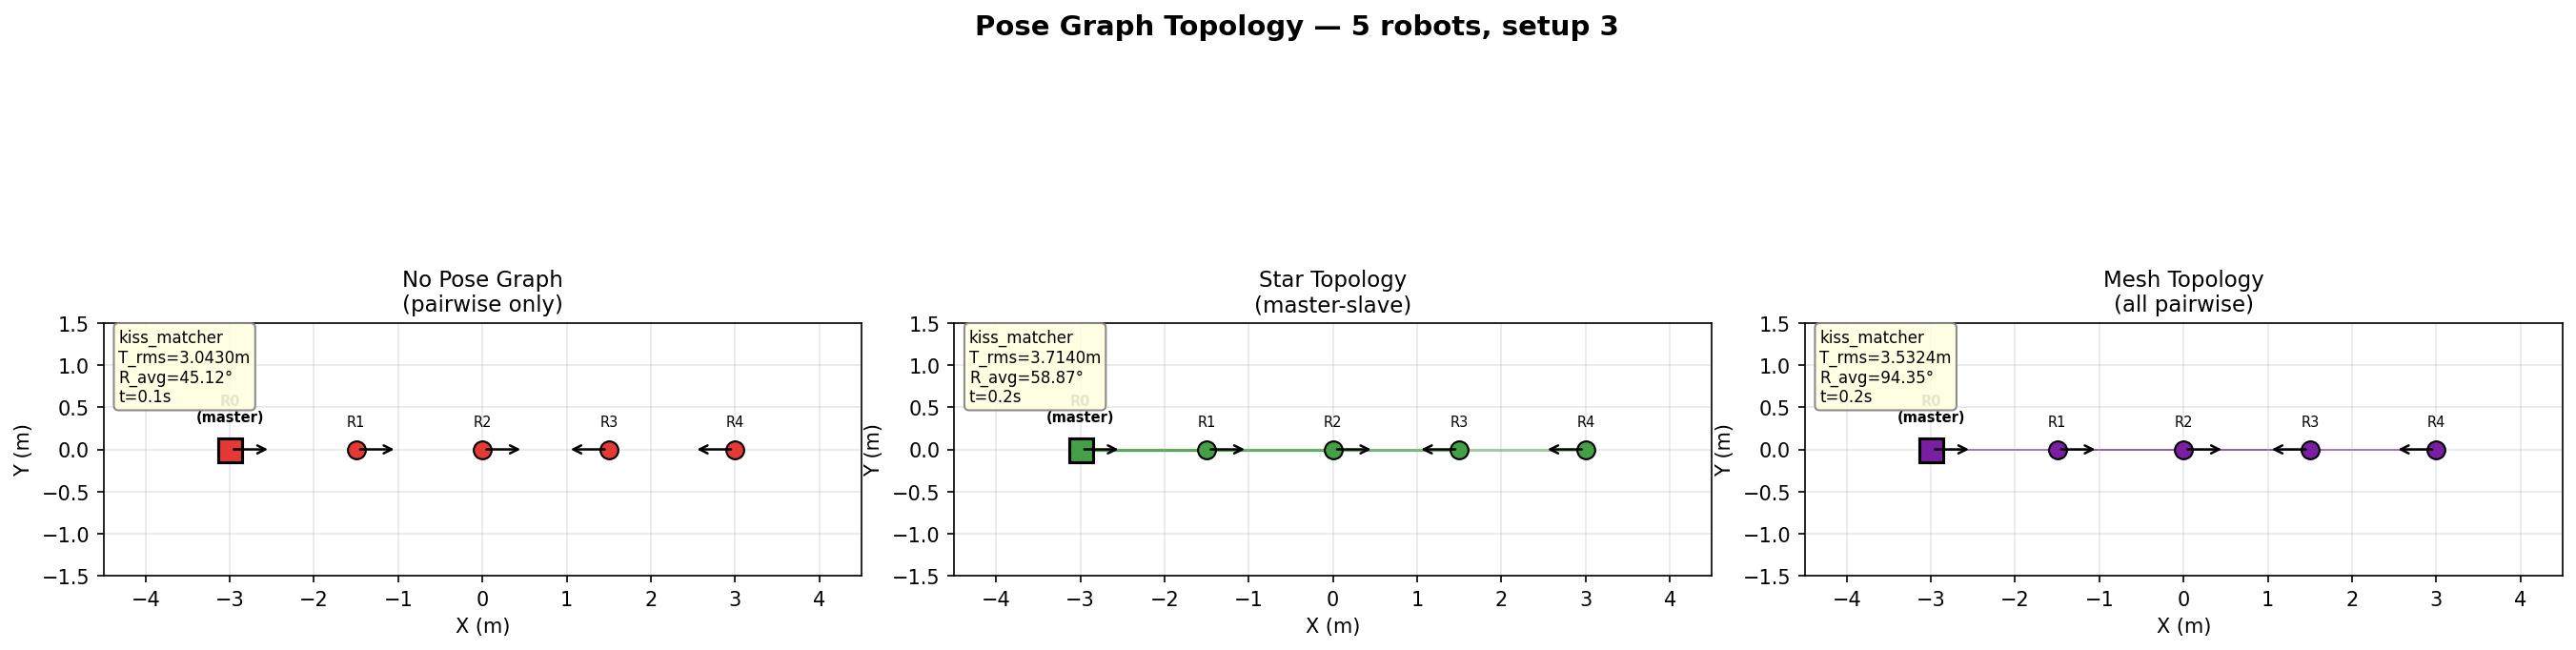
\includegraphics[width=0.7\textwidth]{figures/robots_5_setup_3_pose_graph.png}
    \caption{Pose graph visualization --- 5~robots, Setup~3.}
    \label{fig:app_5r_s3_pg}
\end{figure}

\begin{figure}[htbp]
    \centering
    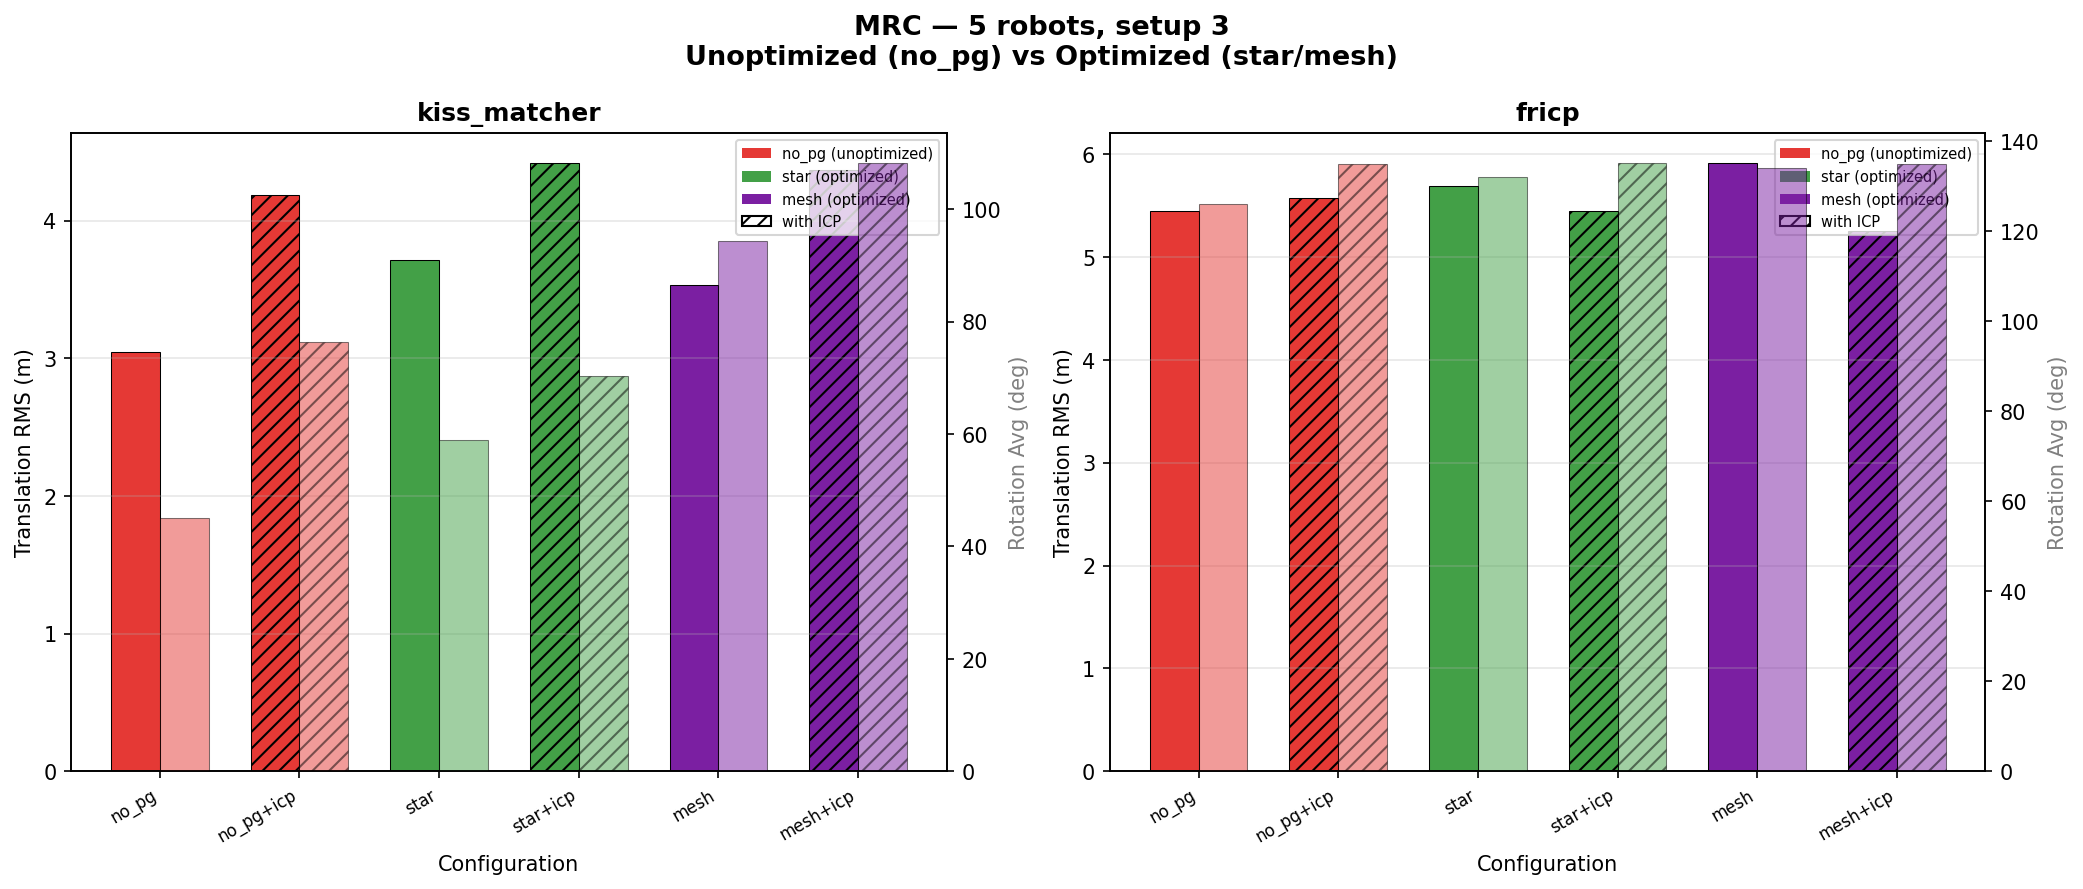
\includegraphics[width=0.95\textwidth]{figures/robots_5_setup_3_unopt_vs_opt.png}
    \caption{Unoptimized vs.\ optimized comparison --- 5~robots, Setup~3.}
    \label{fig:app_5r_s3_unopt}
\end{figure}

%% --- Setup 4 ---
\subsection{Setup~4: Cross/Plus Pattern}

\begin{table}[htbp]
    \centering
    \caption{5~robots, Setup~4 --- cross/plus pattern
             (overlap: 60.3\%).}
    \label{tab:app_5r_s4}
    \small
    \begin{tabular}{l r r r r r}
        \toprule
        \textbf{Configuration}
            & $\bar{e}_t$ [m]
            & $e_t^\mathrm{RMS}$ [m]
            & $\bar{e}_r$ [deg]
            & Ovlp [\%]
            & $t$ [s] \\
        \midrule
        \multicolumn{6}{l}{\textit{KISS-Matcher}} \\
        \quad no PG         & 0.18 & 0.22 &   1.6 & 60.3 &  0.2 \\
        \quad star PG       & 0.29 & 0.33 &   2.6 & 60.3 &  0.1 \\
        \quad mesh PG       & 1.89 & 2.44 &  56.7 & 60.3 &  0.2 \\
        \quad no PG + ICP   & 2.46 & 3.92 &  38.6 & 60.3 &  2.1 \\
        \quad star PG + ICP & 1.47 & 2.59 &  20.1 & 60.3 &  2.7 \\
        \quad mesh PG + ICP & 2.57 & 3.69 &  43.6 & 60.3 &  6.0 \\
        \midrule
        \multicolumn{6}{l}{\textit{FRICP}} \\
        \quad no PG         & 4.62 & 5.21 & 104.5 & 60.3 &  3.9 \\
        \quad star PG       & 5.26 & 5.69 & 124.9 & 60.3 &  3.7 \\
        \quad mesh PG       & 4.78 & 4.92 & 131.4 & 60.3 &  9.2 \\
        \quad no PG + ICP   & 5.39 & 5.64 & 133.8 & 60.3 &  6.6 \\
        \quad star PG + ICP & 5.56 & 5.85 & 134.8 & 60.3 &  6.7 \\
        \quad mesh PG + ICP & 4.85 & 4.95 & 134.5 & 60.3 & 16.8 \\
        \bottomrule
    \end{tabular}
\end{table}

\begin{figure}[htbp]
    \centering
    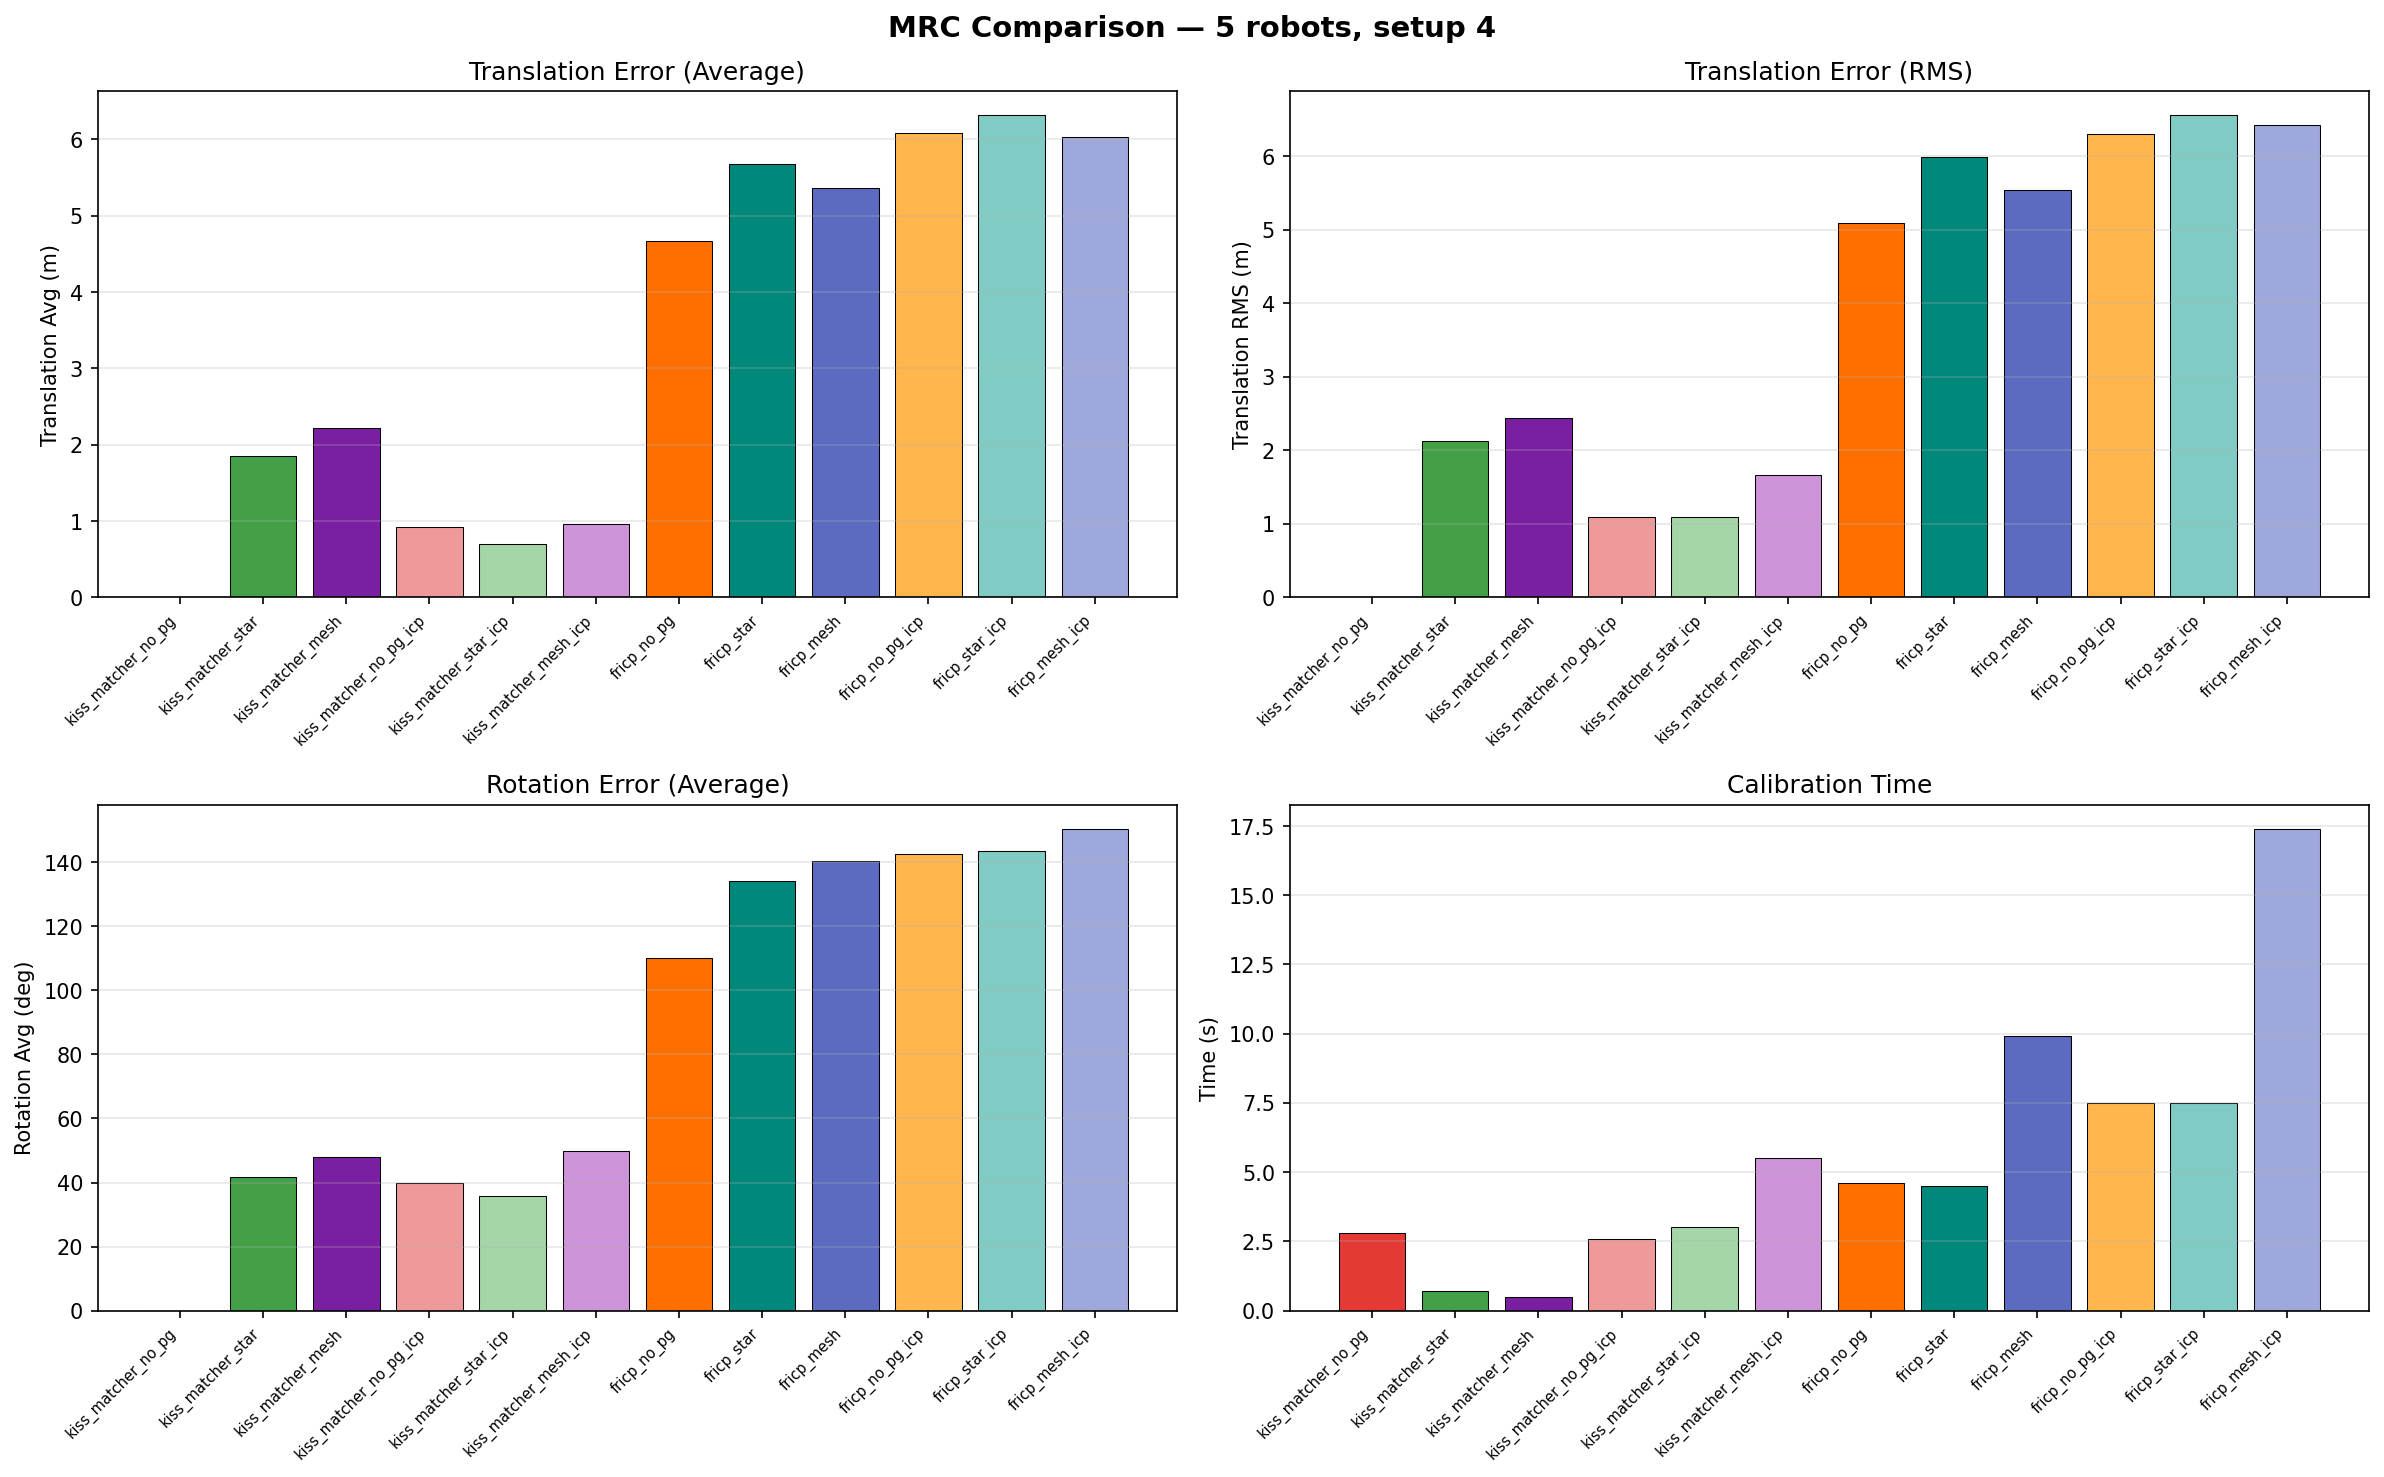
\includegraphics[width=0.95\textwidth]{figures/robots_5_setup_4_bars.png}
    \caption{Configuration comparison --- 5~robots, Setup~4.}
    \label{fig:app_5r_s4_bars}
\end{figure}

\begin{figure}[htbp]
    \centering
    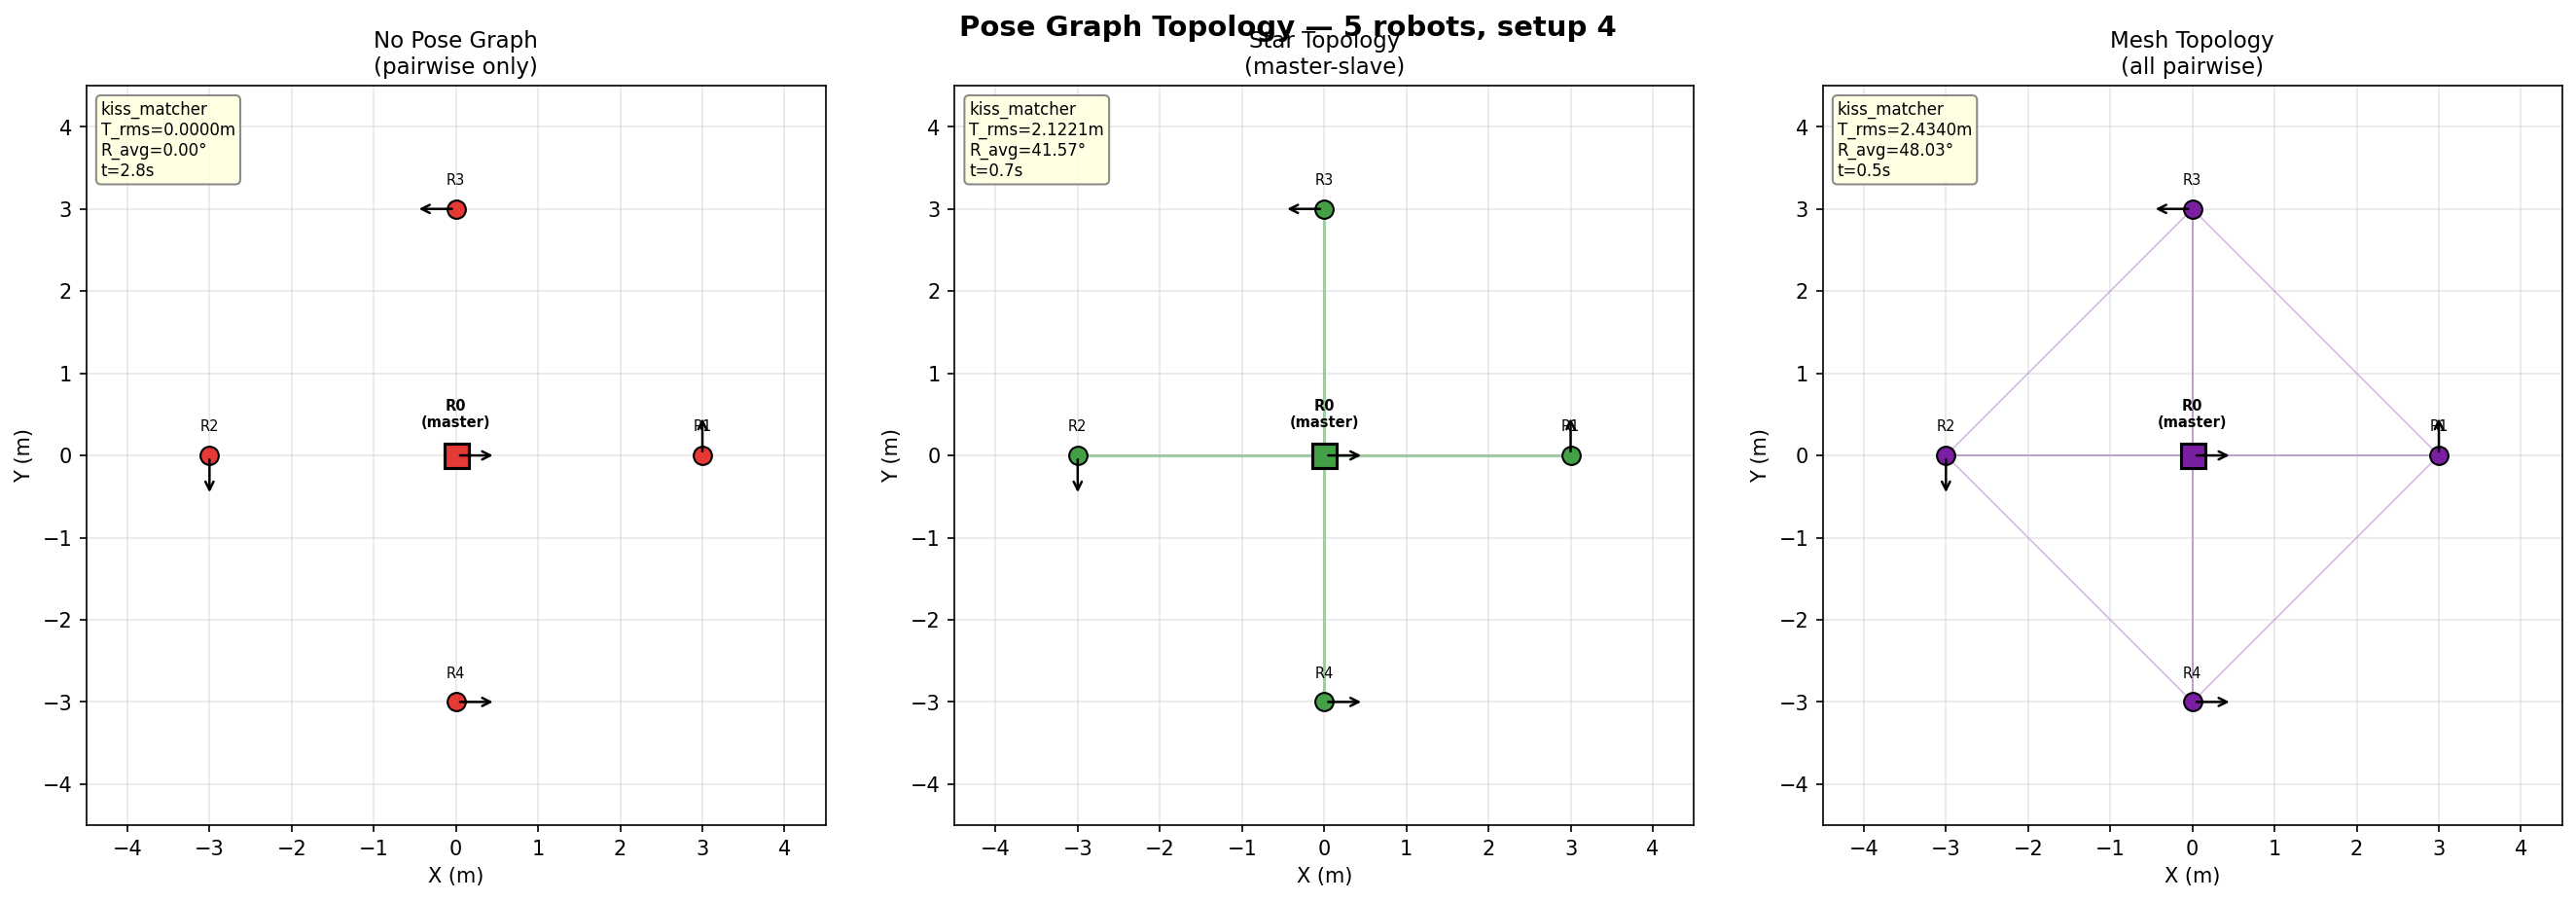
\includegraphics[width=0.7\textwidth]{figures/robots_5_setup_4_pose_graph.png}
    \caption{Pose graph visualization --- 5~robots, Setup~4.}
    \label{fig:app_5r_s4_pg}
\end{figure}

\begin{figure}[htbp]
    \centering
    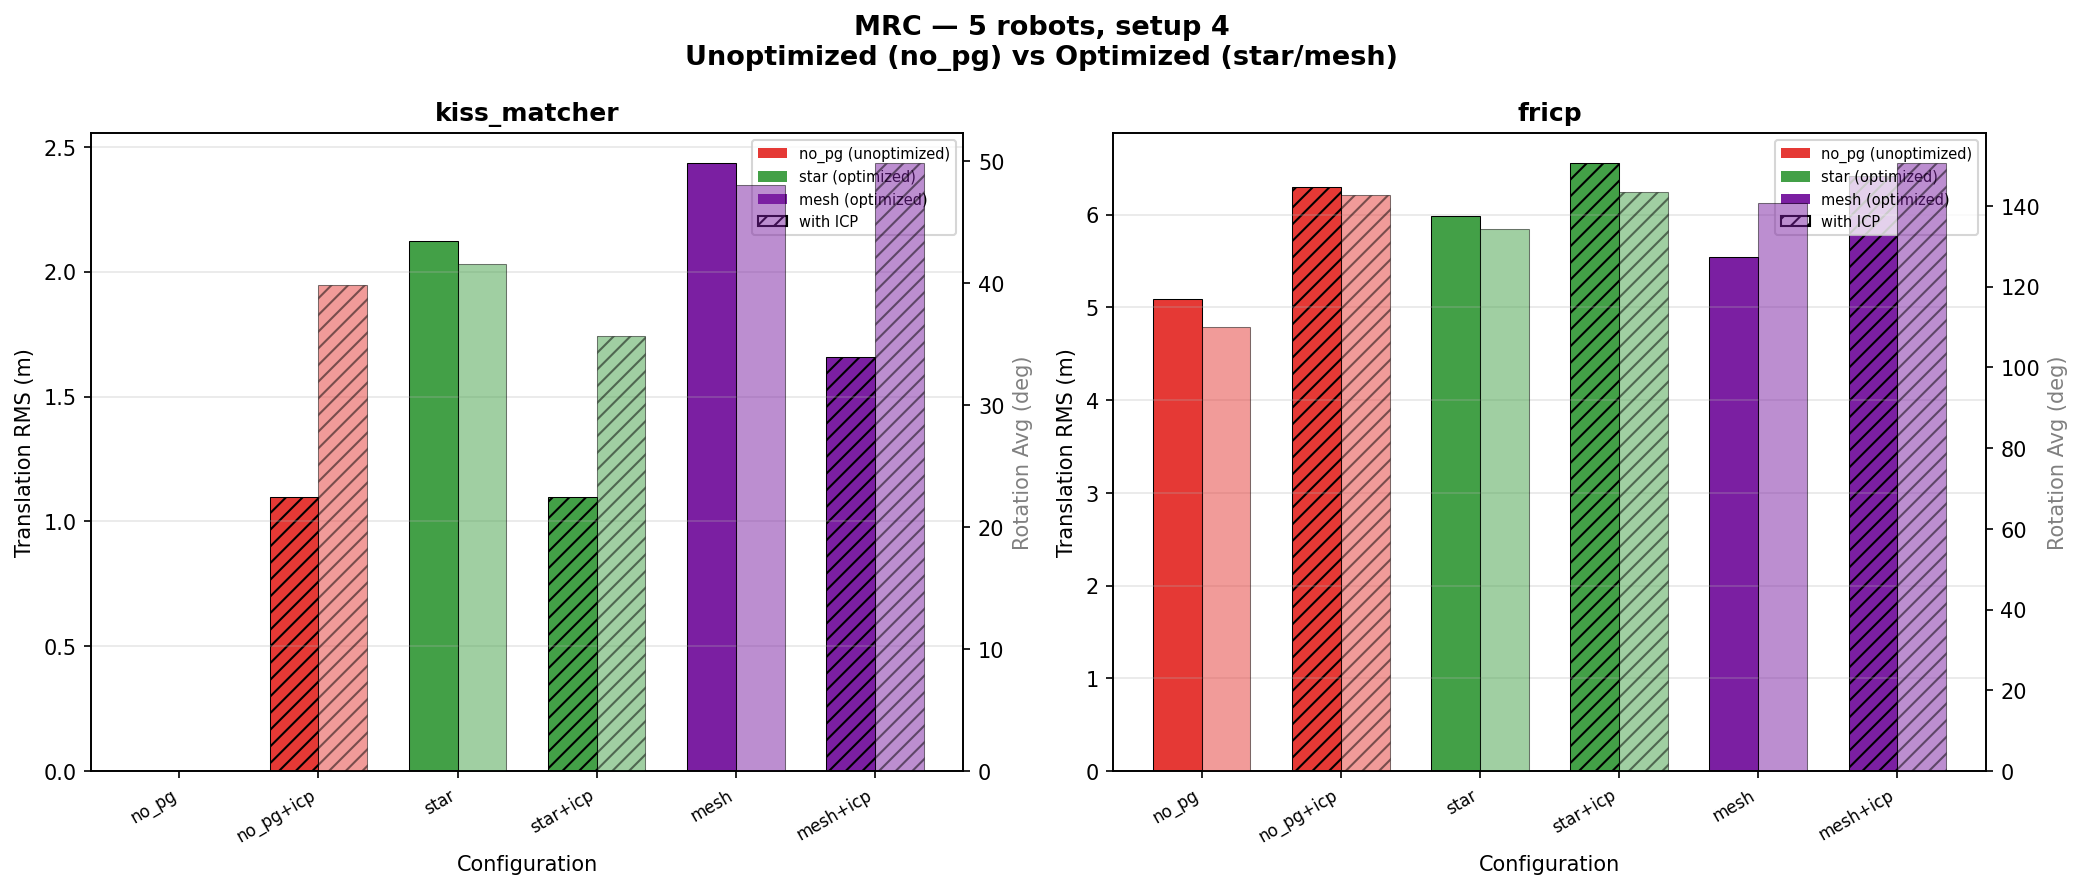
\includegraphics[width=0.95\textwidth]{figures/robots_5_setup_4_unopt_vs_opt.png}
    \caption{Unoptimized vs.\ optimized comparison --- 5~robots, Setup~4.}
    \label{fig:app_5r_s4_unopt}
\end{figure}

%% --- Setup 5 ---
\subsection{Setup~5: Scattered Asymmetric}

\begin{table}[htbp]
    \centering
    \caption{5~robots, Setup~5 --- scattered asymmetric
             (overlap: 50.4\%).}
    \label{tab:app_5r_s5}
    \small
    \begin{tabular}{l r r r r r}
        \toprule
        \textbf{Configuration}
            & $\bar{e}_t$ [m]
            & $e_t^\mathrm{RMS}$ [m]
            & $\bar{e}_r$ [deg]
            & Ovlp [\%]
            & $t$ [s] \\
        \midrule
        \multicolumn{6}{l}{\textit{KISS-Matcher}} \\
        \quad no PG         &  3.96 &  4.97 &  59.9 & 50.4 &  0.2 \\
        \quad star PG       &  4.92 &  6.43 &  65.1 & 50.4 &  0.2 \\
        \quad mesh PG       &  6.41 &  8.31 &  89.3 & 50.4 &  0.2 \\
        \quad no PG + ICP   &  7.08 &  8.83 &  84.9 & 50.4 &  2.4 \\
        \quad star PG + ICP &  6.52 &  7.83 &  89.9 & 50.4 &  1.7 \\
        \quad mesh PG + ICP &  7.01 &  8.40 &  60.0 & 50.4 &  3.5 \\
        \midrule
        \multicolumn{6}{l}{\textit{FRICP}} \\
        \quad no PG         &  7.90 &  8.57 & 127.7 & 50.4 &  5.6 \\
        \quad star PG       &  8.21 &  8.63 & 151.2 & 50.4 &  5.6 \\
        \quad mesh PG       &  8.61 &  8.86 & 146.7 & 50.4 & 13.6 \\
        \quad no PG + ICP   &  8.24 &  8.46 & 160.8 & 50.4 &  9.9 \\
        \quad star PG + ICP &  8.18 &  8.38 & 162.7 & 50.4 &  9.8 \\
        \quad mesh PG + ICP &  8.15 &  8.32 & 152.5 & 50.4 & 23.0 \\
        \bottomrule
    \end{tabular}
\end{table}

\begin{figure}[htbp]
    \centering
    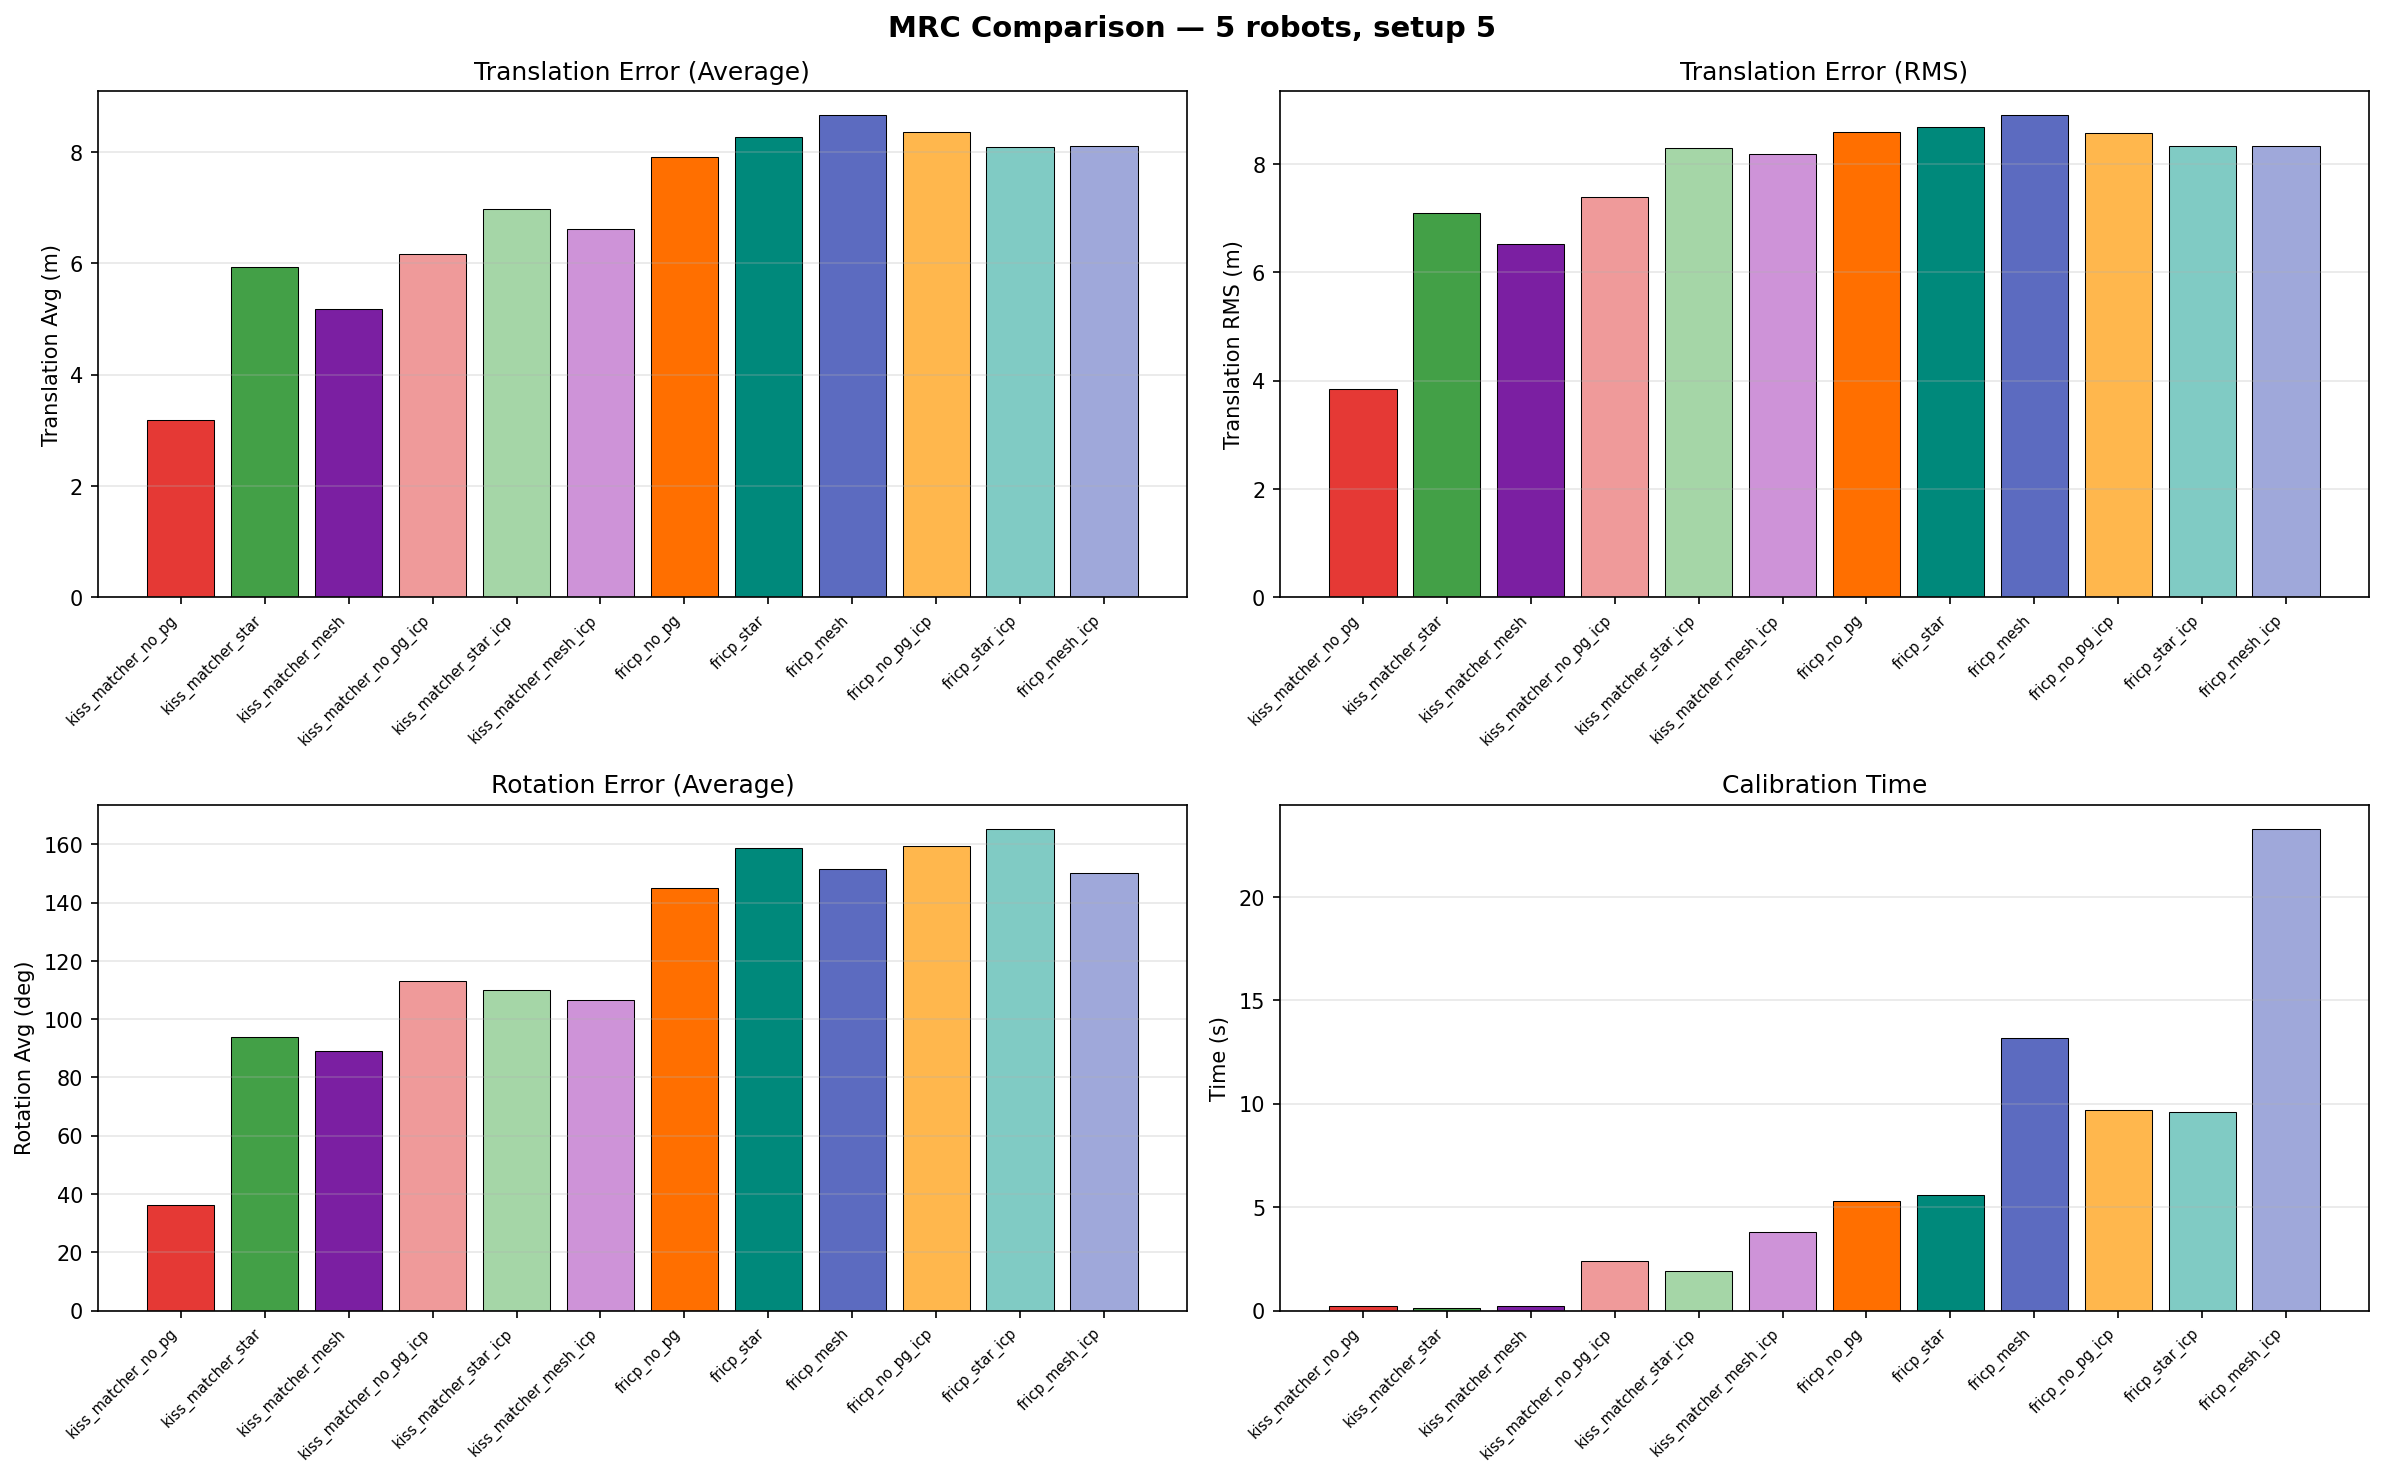
\includegraphics[width=0.95\textwidth]{figures/robots_5_setup_5_bars.png}
    \caption{Configuration comparison --- 5~robots, Setup~5.}
    \label{fig:app_5r_s5_bars}
\end{figure}

\begin{figure}[htbp]
    \centering
    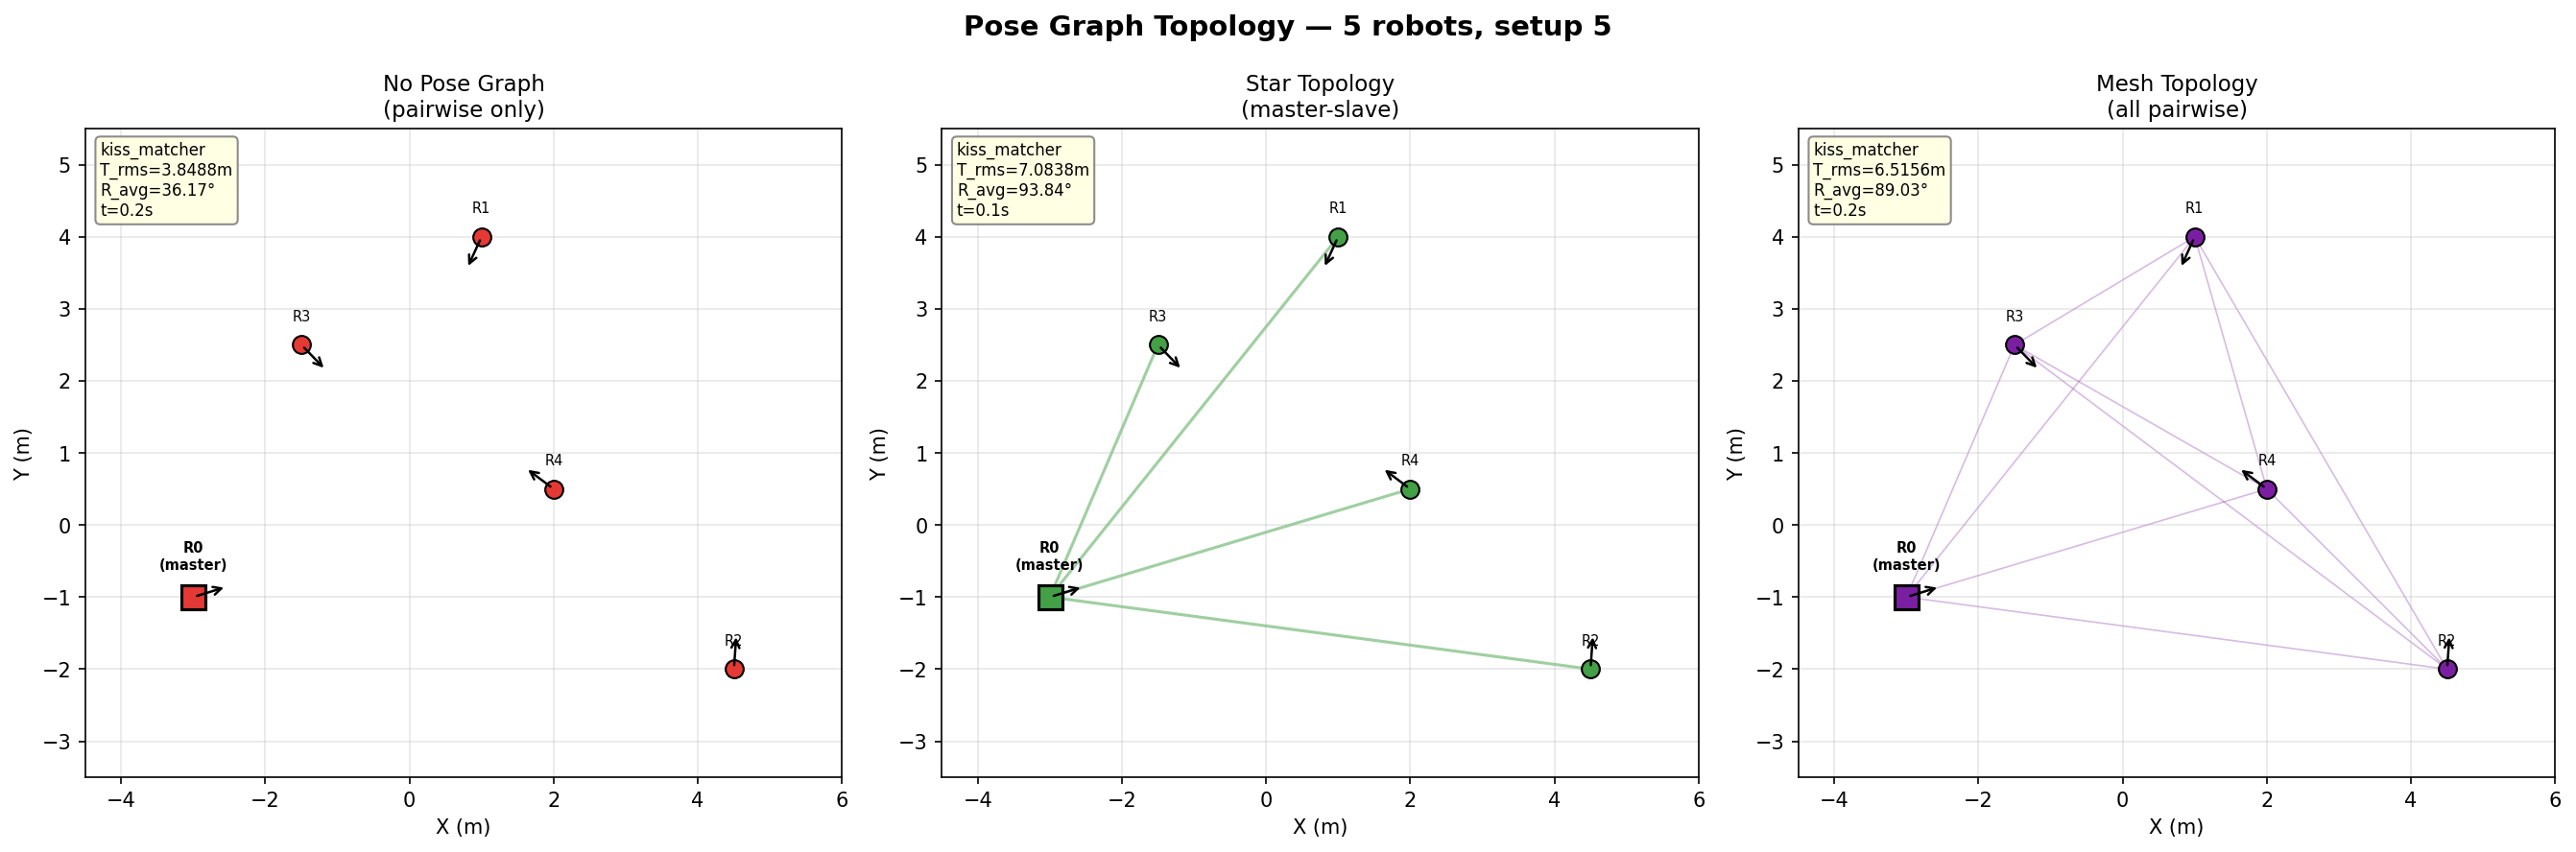
\includegraphics[width=0.7\textwidth]{figures/robots_5_setup_5_pose_graph.png}
    \caption{Pose graph visualization --- 5~robots, Setup~5.}
    \label{fig:app_5r_s5_pg}
\end{figure}

\begin{figure}[htbp]
    \centering
    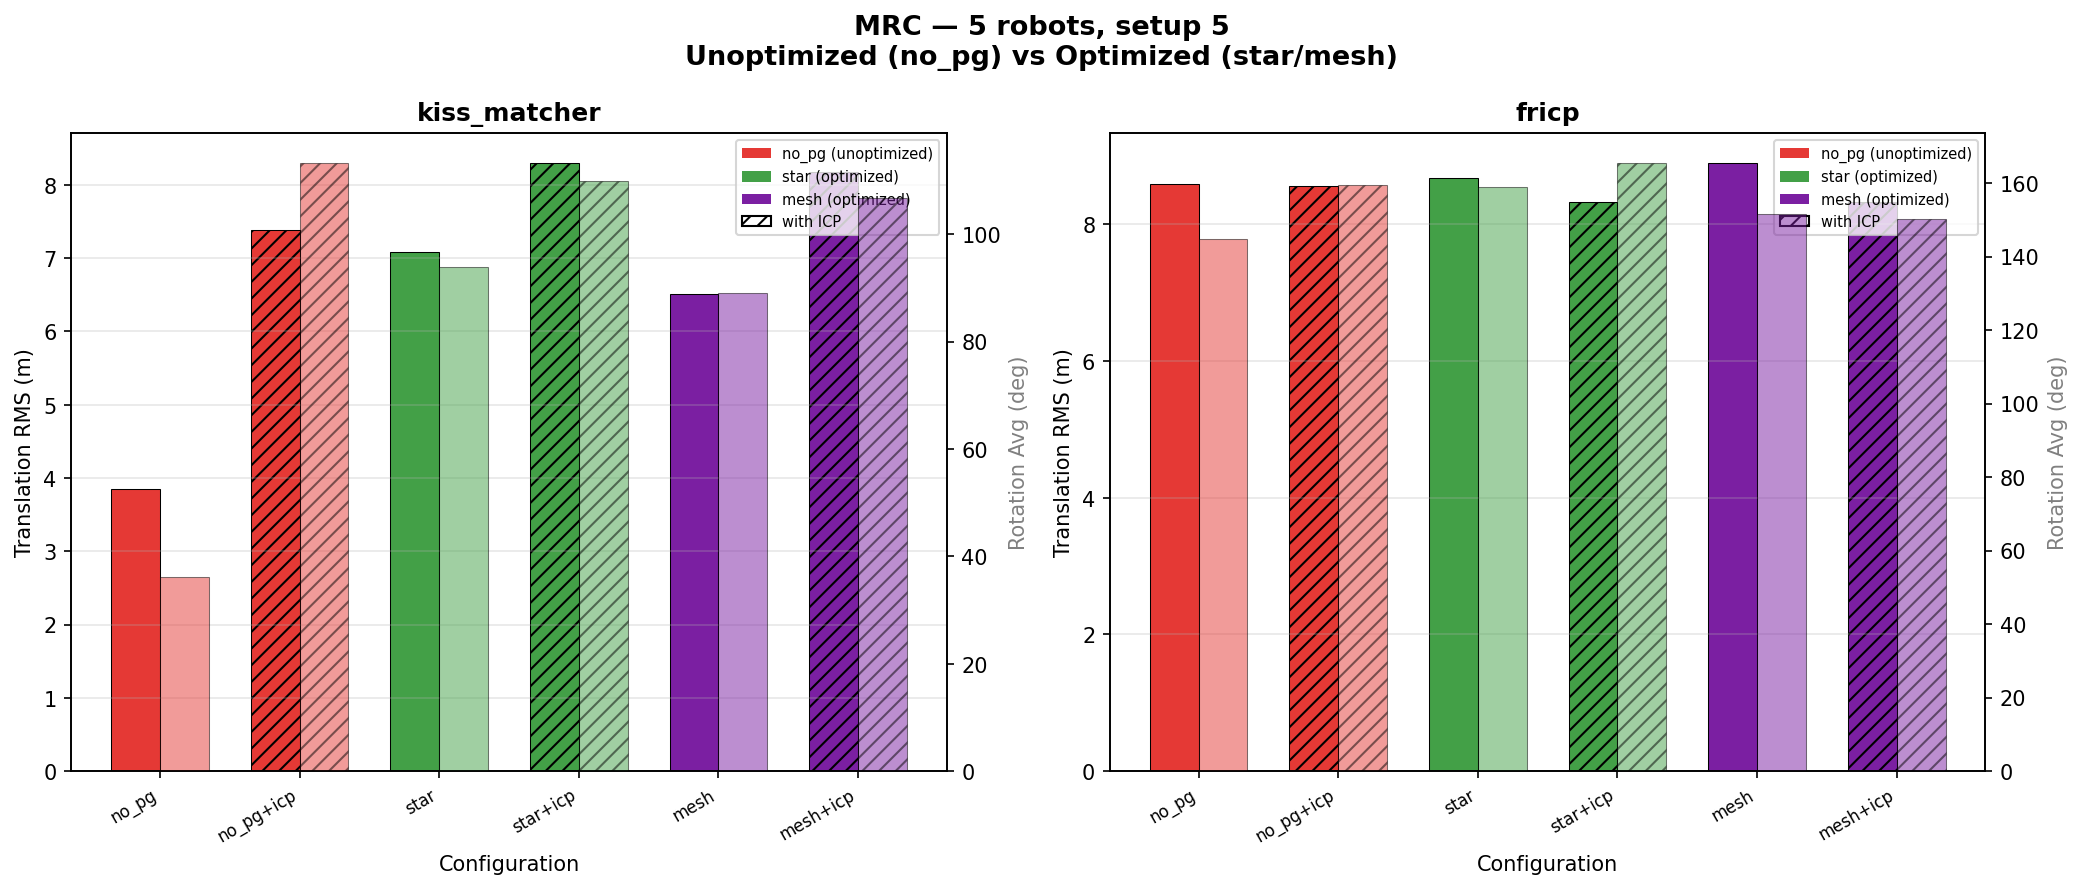
\includegraphics[width=0.95\textwidth]{figures/robots_5_setup_5_unopt_vs_opt.png}
    \caption{Unoptimized vs.\ optimized comparison --- 5~robots, Setup~5.}
    \label{fig:app_5r_s5_unopt}
\end{figure}

%% --- 5-robot averaged ---
\subsection{Averaged Results (5~Robots)}

\begin{table}[htbp]
    \centering
    \caption{5~robots --- averaged over all 5 position setups
             (3 trials per configuration).}
    \label{tab:app_5r_avg}
    \small
    \begin{tabular}{l r r r r r}
        \toprule
        \textbf{Configuration}
            & $\bar{e}_t$ [m]
            & $e_t^\mathrm{RMS}$ [m]
            & $\bar{e}_r$ [deg]
            & Ovlp [\%]
            & $t$ [s] \\
        \midrule
        \multicolumn{6}{l}{\textit{KISS-Matcher}} \\
        \quad no PG         & \textbf{3.67} & \textbf{4.38} &  59.4 & 48.5 &  0.3 \\
        \quad star PG       & 4.16 &  5.11 &  58.0 & 48.5 &  0.3 \\
        \quad mesh PG       & 5.24 &  6.24 &  83.6 & 48.5 &  0.3 \\
        \quad no PG + ICP   & 5.49 &  6.88 &  81.9 & 48.5 &  2.5 \\
        \quad star PG + ICP & 5.15 &  6.38 &  74.7 & 48.5 &  2.7 \\
        \quad mesh PG + ICP & 5.16 &  6.16 &  72.6 & 48.5 &  5.5 \\
        \midrule
        \multicolumn{6}{l}{\textit{FRICP}} \\
        \quad no PG         & 6.24 &  6.92 & 133.3 & 48.5 &  4.3 \\
        \quad star PG       & 6.71 &  7.25 & 151.9 & 48.5 &  4.2 \\
        \quad mesh PG       & 6.85 &  7.24 & 150.0 & 48.5 & 11.2 \\
        \quad no PG + ICP   & 6.84 &  7.31 & 159.2 & 48.5 &  7.5 \\
        \quad star PG + ICP & 6.79 &  7.32 & 160.4 & 48.5 &  7.6 \\
        \quad mesh PG + ICP & 6.60 &  7.10 & 154.8 & 48.5 & 19.5 \\
        \bottomrule
    \end{tabular}
\end{table}

\subsection{Cross-Setup Summary (5~Robots)}

\begin{figure}[htbp]
    \centering
    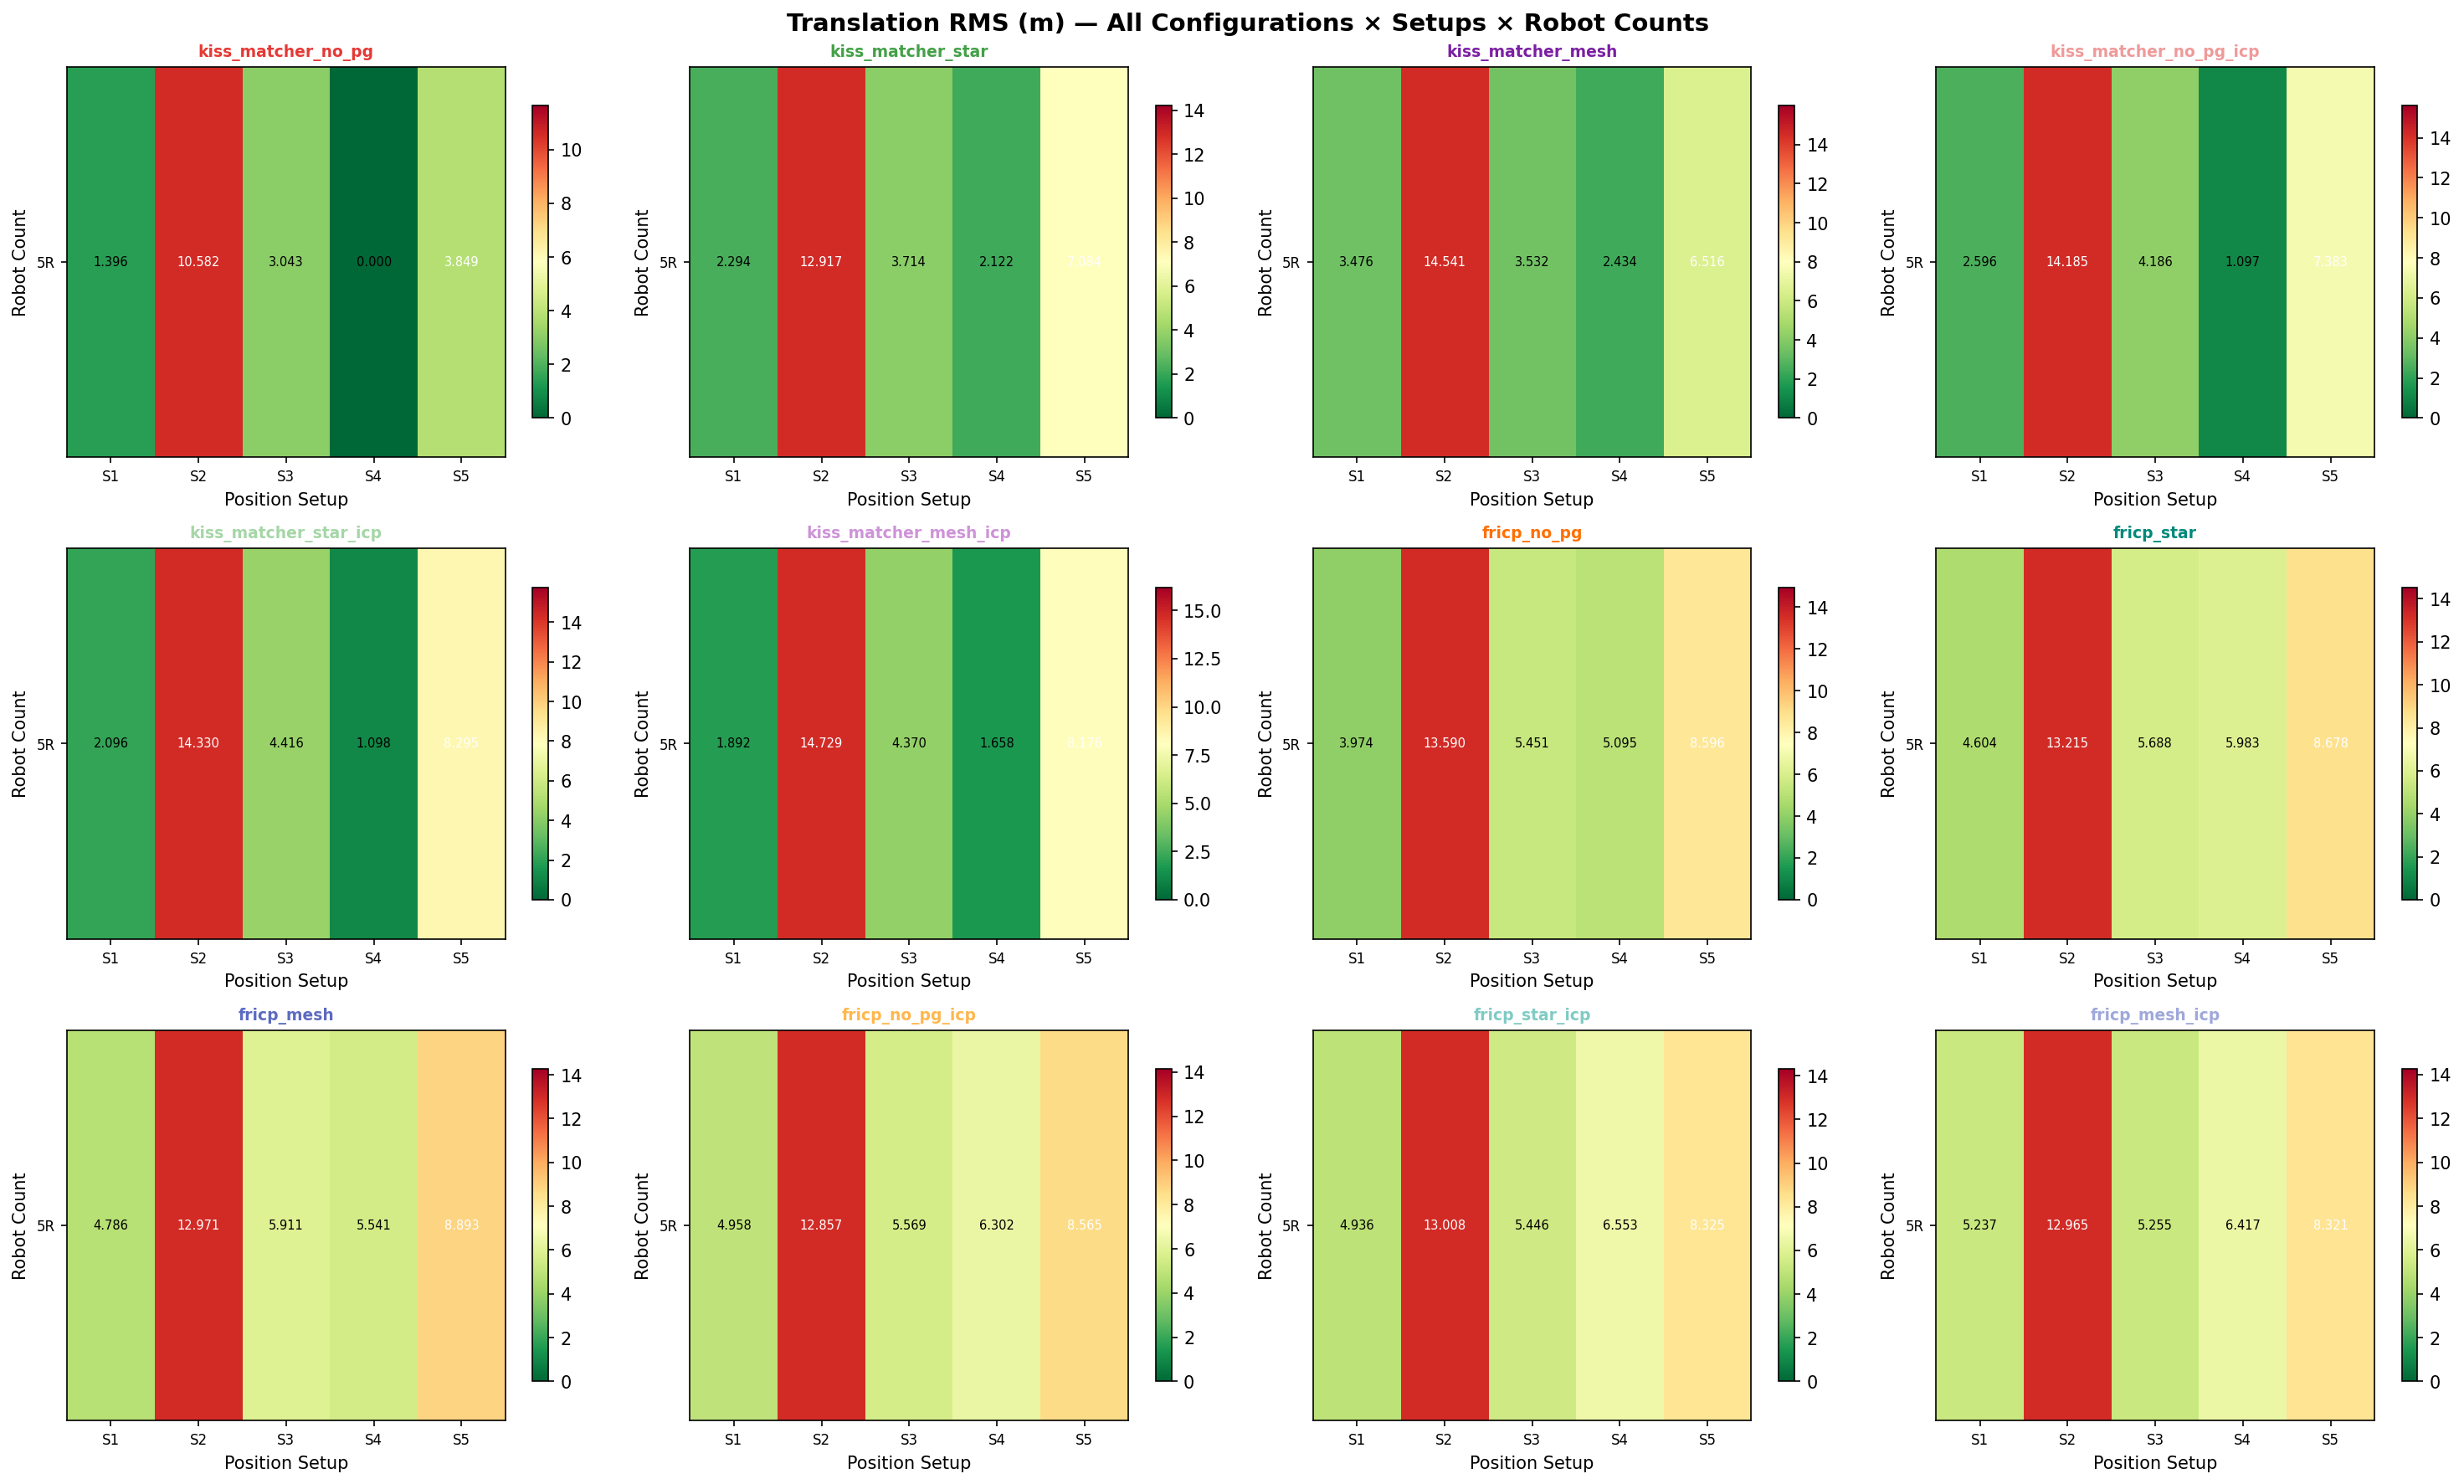
\includegraphics[width=\textwidth]{figures/heatmap_5_robots.png}
    \caption{Heatmap of translation RMS across position setups
             for all 12 configurations (5~robots).}
    \label{fig:app_5r_heatmap}
\end{figure}

\begin{figure}[htbp]
    \centering
    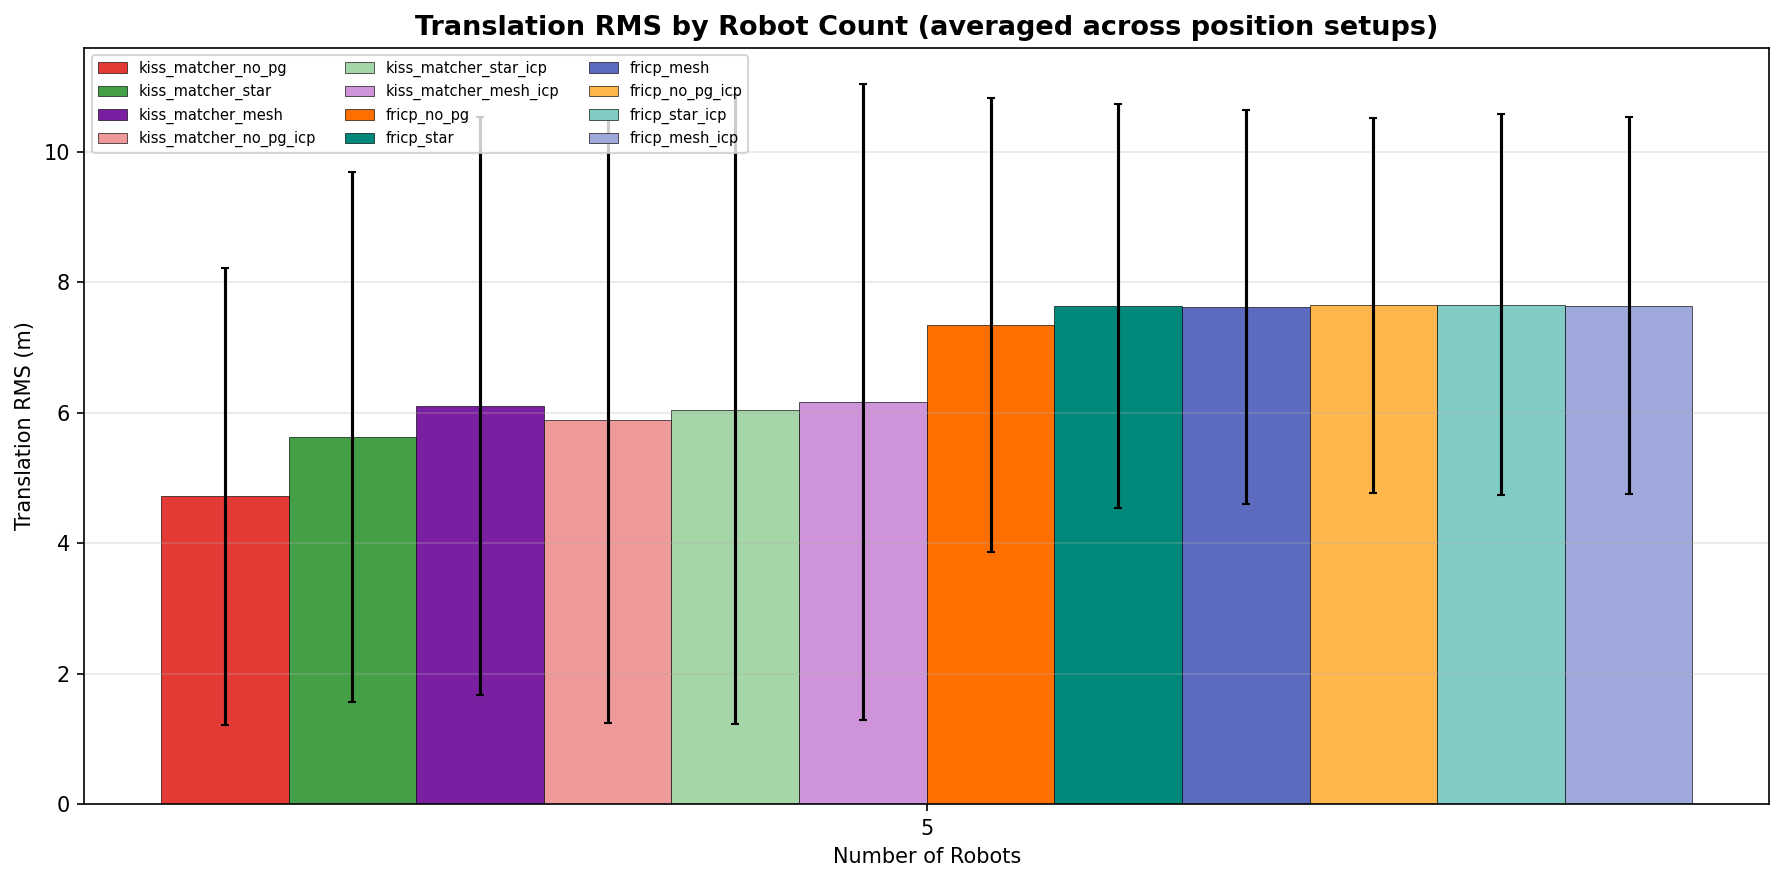
\includegraphics[width=\textwidth]{figures/summary_5_robots.png}
    \caption{Summary of translation RMS by configuration (5~robots).}
    \label{fig:app_5r_summary}
\end{figure}

%% ---------------------------------------------------------------------------
\section{10-Robot Scalability Tests (Partial)}
\label{sec:app_10robots}

Ten homogeneous EC~Swift robots were deployed in the scalability
test world ($20 \times 20$\,m room, reduced physics).
Due to Zenoh middleware transport saturation, only Setup~2 produced
partial results (7 of 12 configurations completed before the
\SI{1000}{\second} timeout).
Setups~3--5 failed entirely (robots did not spawn), and Setup~1
timed out with no completed configurations.

%% --- Setup 2 (partial) ---
\subsection{Setup~2: Wide Regular Decagon (Partial)}

\begin{table}[htbp]
    \centering
    \caption{10~robots, Setup~2 --- wide regular decagon
             ($r = \SI{5}{\metre}$, overlap: 2.1\%).
             Only configurations that completed at least one
             trial are shown.}
    \label{tab:app_10r_s2}
    \small
    \begin{tabular}{l r r r r}
        \toprule
        \textbf{Configuration}
            & $\bar{e}_t$ [m]
            & $\bar{e}_r$ [deg]
            & Ovlp [\%]
            & $t$ [s] \\
        \midrule
        KM mesh PG + ICP    & 8.37 &  87.4 & 2.1 & 49.8 \\
        \midrule
        FRICP no PG         & 8.44 &  99.6 & 2.1 & 10.9 \\
        FRICP star PG       & 8.49 & 100.4 & 2.1 & 10.7 \\
        FRICP mesh PG       & 8.40 &  99.5 & 2.1 & 58.2 \\
        FRICP no PG + ICP   & 8.17 & 102.1 & 2.1 & 16.9 \\
        FRICP star PG + ICP & 8.03 &  97.2 & 2.1 & 17.0 \\
        \bottomrule
    \end{tabular}
\end{table}

%% ---------------------------------------------------------------------------
\section{2-Robot Proximity Tests}
\label{sec:app_2robots}

Two homogeneous EC~Swift robots with front and back LiDARs
($360\degree$ coverage) were placed in side-by-side proximity
configurations.

\paragraph{Note on Setup~1.}
Setup~1 exhibited a simulation anomaly with 0\% point cloud
overlap despite \SI{1.5}{\metre} robot separation.
KISS-Matcher without ICP produced no valid registrations.
All other configurations produced errors exceeding \SI{4}{\metre}.
Setup~1 data is included below for completeness but is excluded
from the averaged results.

%% --- Setup 1 (anomalous) ---
\subsection{Setup~1: Parallel, No Noise (Anomalous)}

\begin{table}[htbp]
    \centering
    \caption{2~robots, Setup~1 --- parallel at \SI{1.5}{\metre}.
             \textbf{Anomalous:} 0\% overlap, data unreliable.
             Entries marked ``---'' produced no valid registrations.}
    \label{tab:app_2r_s1}
    \small
    \begin{tabular}{l r r r r}
        \toprule
        \textbf{Configuration}
            & $\bar{e}_t$ [m]
            & $\bar{e}_r$ [deg]
            & Ovlp [\%]
            & $t$ [s] \\
        \midrule
        \multicolumn{5}{l}{\textit{KISS-Matcher}} \\
        \quad no PG         & ---    & ---    & 0.0 & 0.1 \\
        \quad star PG       & ---    & ---    & 0.0 & 0.1 \\
        \quad mesh PG       & ---    & ---    & 0.0 & 0.1 \\
        \quad no PG + ICP   & 10.59  &  74.9  & 0.0 & 0.3 \\
        \quad star PG + ICP &  6.24  & 132.8  & 0.0 & 0.6 \\
        \quad mesh PG + ICP &  4.80  & 145.9  & 0.0 & 0.6 \\
        \midrule
        \multicolumn{5}{l}{\textit{FRICP}} \\
        \quad no PG         &  6.36  &  65.6  & 0.0 & 0.9 \\
        \quad star PG       &  7.01  &  38.5  & 0.0 & 0.8 \\
        \quad mesh PG       &  6.68  &  18.4  & 0.0 & 0.9 \\
        \quad no PG + ICP   &  6.54  &  11.2  & 0.0 & 1.7 \\
        \quad star PG + ICP &  6.68  &   9.5  & 0.0 & 1.9 \\
        \quad mesh PG + ICP &  6.53  &   8.6  & 0.0 & 1.9 \\
        \bottomrule
    \end{tabular}
\end{table}

%% --- Setup 2 ---
\subsection{Setup~2: Slight Offset + Yaw}

\begin{table}[htbp]
    \centering
    \caption{2~robots, Setup~2 --- slight offset at \SI{1.0}{\metre}
             with $\Delta\psi = 2.9\degree$
             (overlap: 69.1\%).}
    \label{tab:app_2r_s2}
    \small
    \begin{tabular}{l r r r r}
        \toprule
        \textbf{Configuration}
            & $\bar{e}_t$ [mm]
            & $\bar{e}_r$ [deg]
            & Ovlp [\%]
            & $t$ [s] \\
        \midrule
        \multicolumn{5}{l}{\textit{KISS-Matcher}} \\
        \quad no PG         &  79.8 & 0.91 & 69.1 & 0.1 \\
        \quad star PG       & 108.3 & 0.97 & 69.1 & 0.1 \\
        \quad mesh PG       & 135.1 & 1.17 & 69.1 & 0.1 \\
        \quad no PG + ICP   &  58.2 & 0.53 & 69.1 & 0.6 \\
        \quad star PG + ICP &  44.0 & 0.30 & 69.1 & 0.6 \\
        \quad mesh PG + ICP &  32.1 & 0.23 & 69.1 & 0.6 \\
        \midrule
        \multicolumn{5}{l}{\textit{FRICP}} \\
        \quad no PG         &  15.1 & 0.09 & 69.1 & 0.7 \\
        \quad star PG       &   7.4 & 0.04 & 69.1 & 0.7 \\
        \quad mesh PG       &   4.5 & 0.03 & 69.1 & 0.8 \\
        \quad no PG + ICP   &  21.9 & 0.11 & 69.1 & 1.2 \\
        \quad star PG + ICP &  22.0 & 0.14 & 69.1 & 1.2 \\
        \quad mesh PG + ICP &  22.5 & 0.24 & 69.1 & 1.2 \\
        \bottomrule
    \end{tabular}
\end{table}

\begin{figure}[htbp]
    \centering
    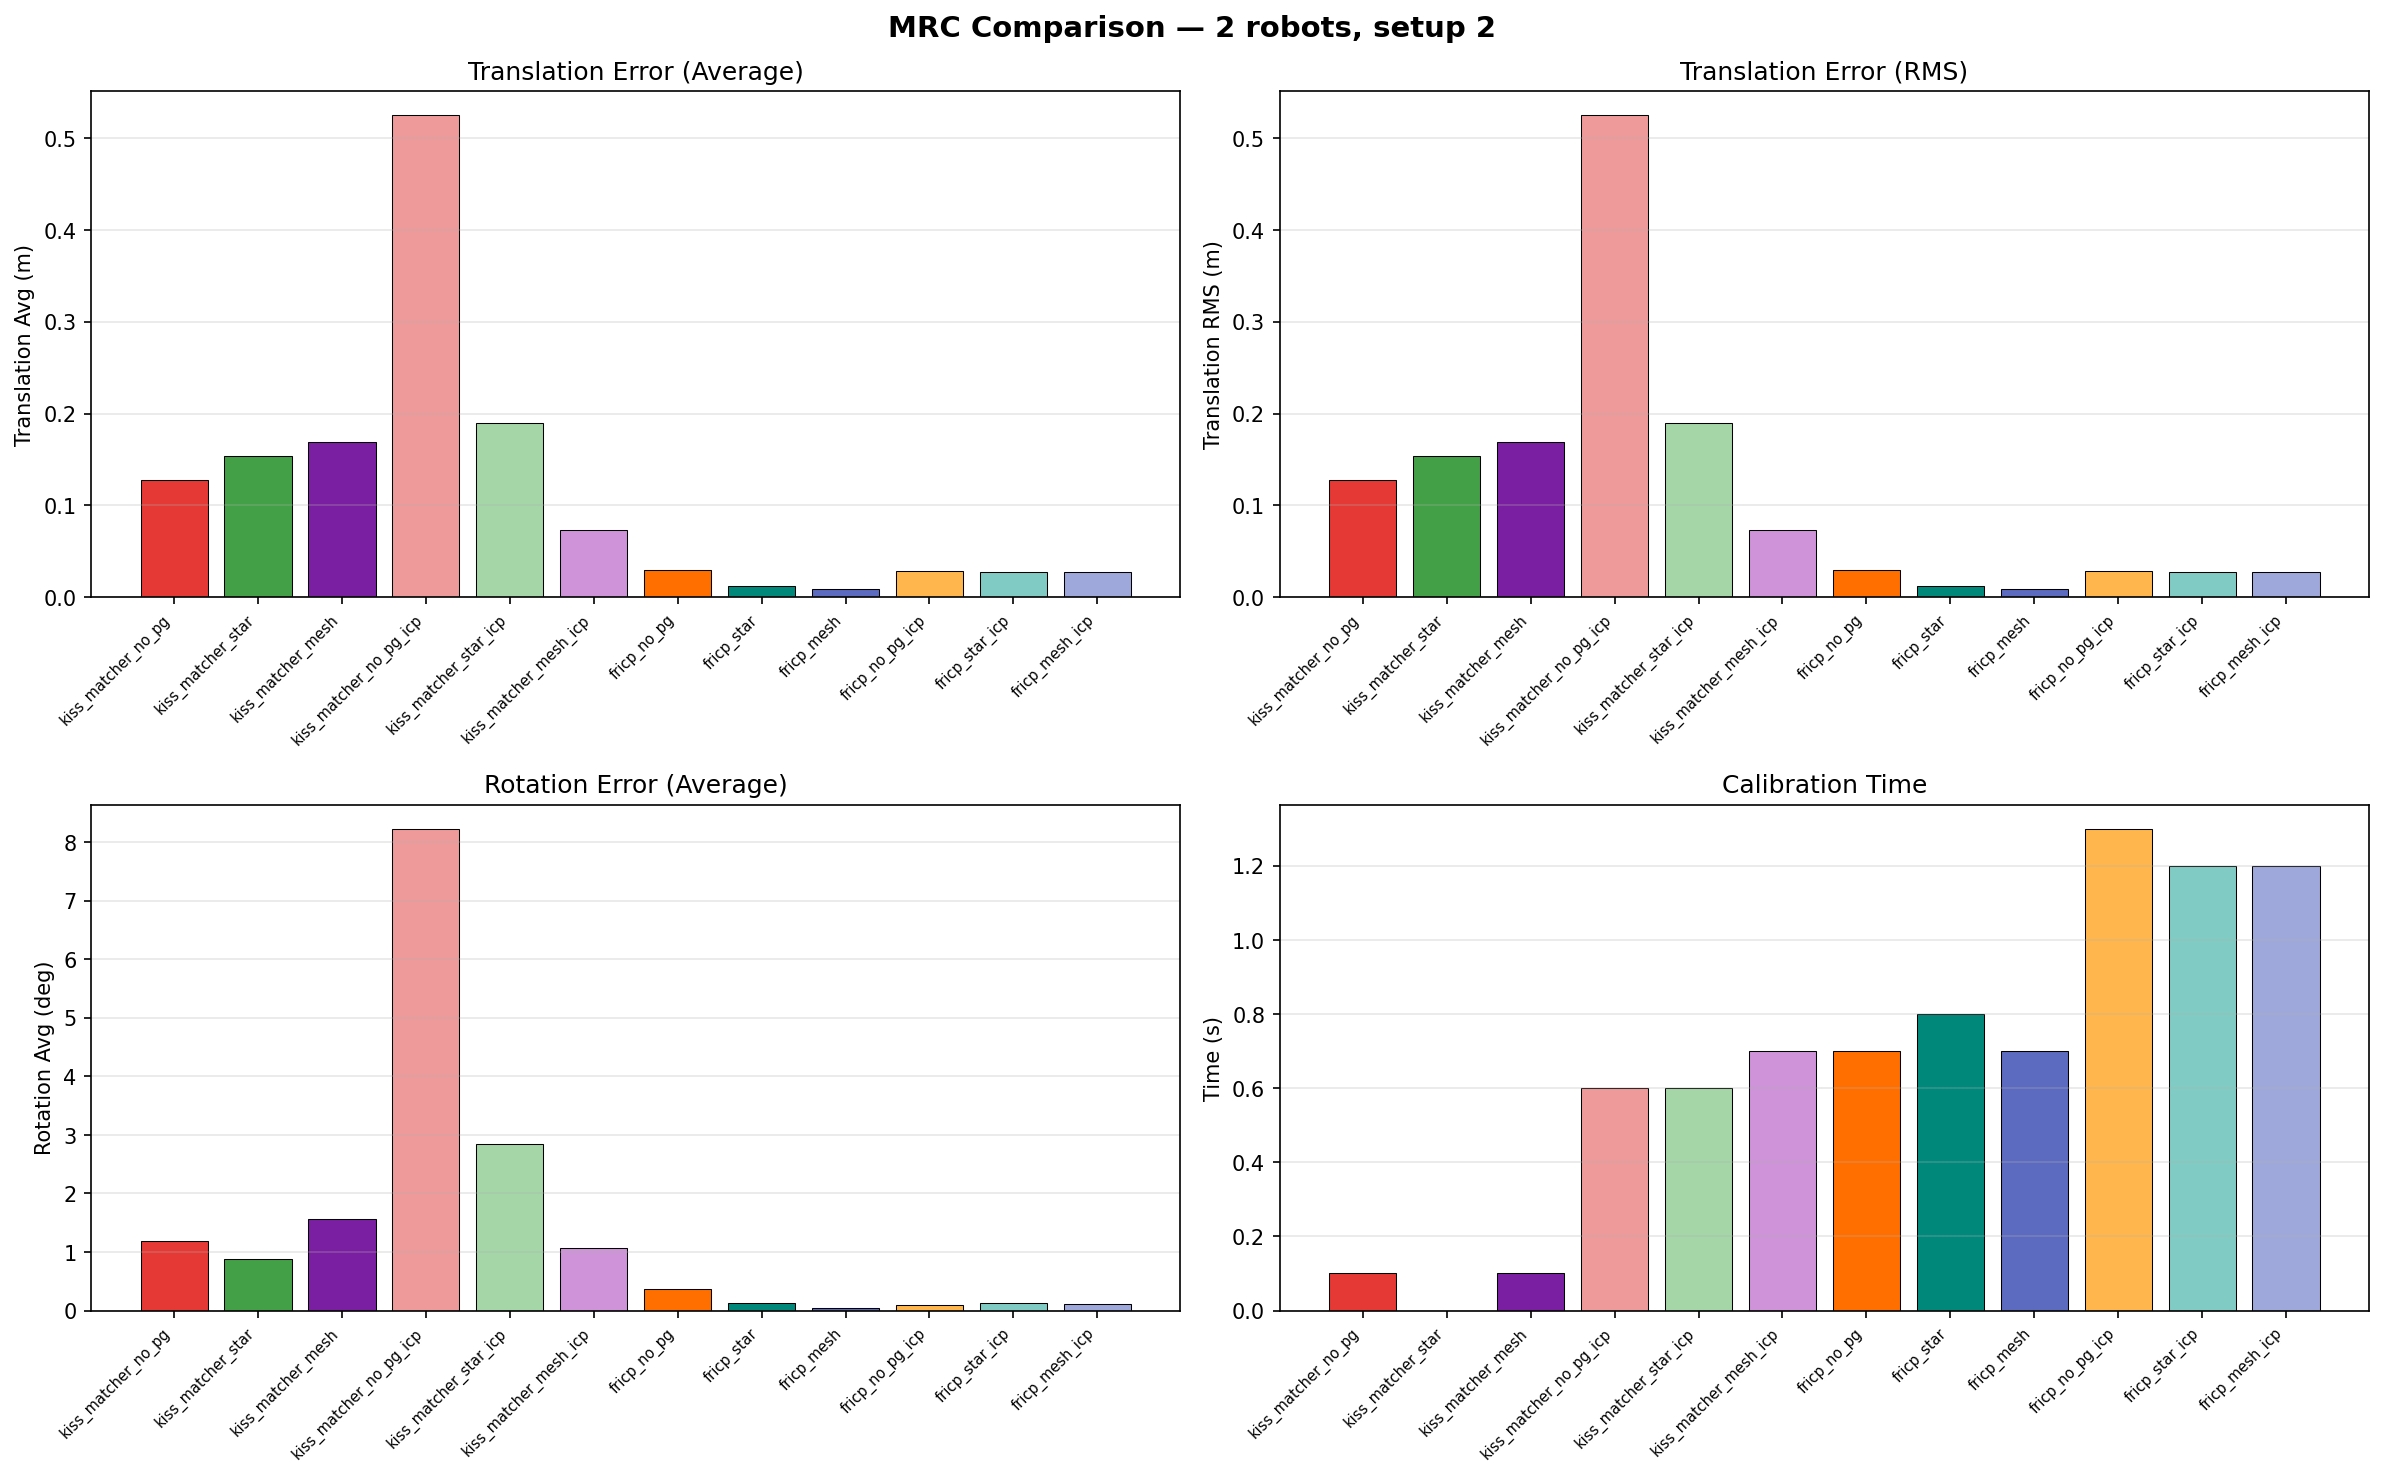
\includegraphics[width=0.95\textwidth]{figures/robots_2_setup_2_bars.png}
    \caption{Configuration comparison --- 2~robots, Setup~2.}
    \label{fig:app_2r_s2_bars}
\end{figure}

\begin{figure}[htbp]
    \centering
    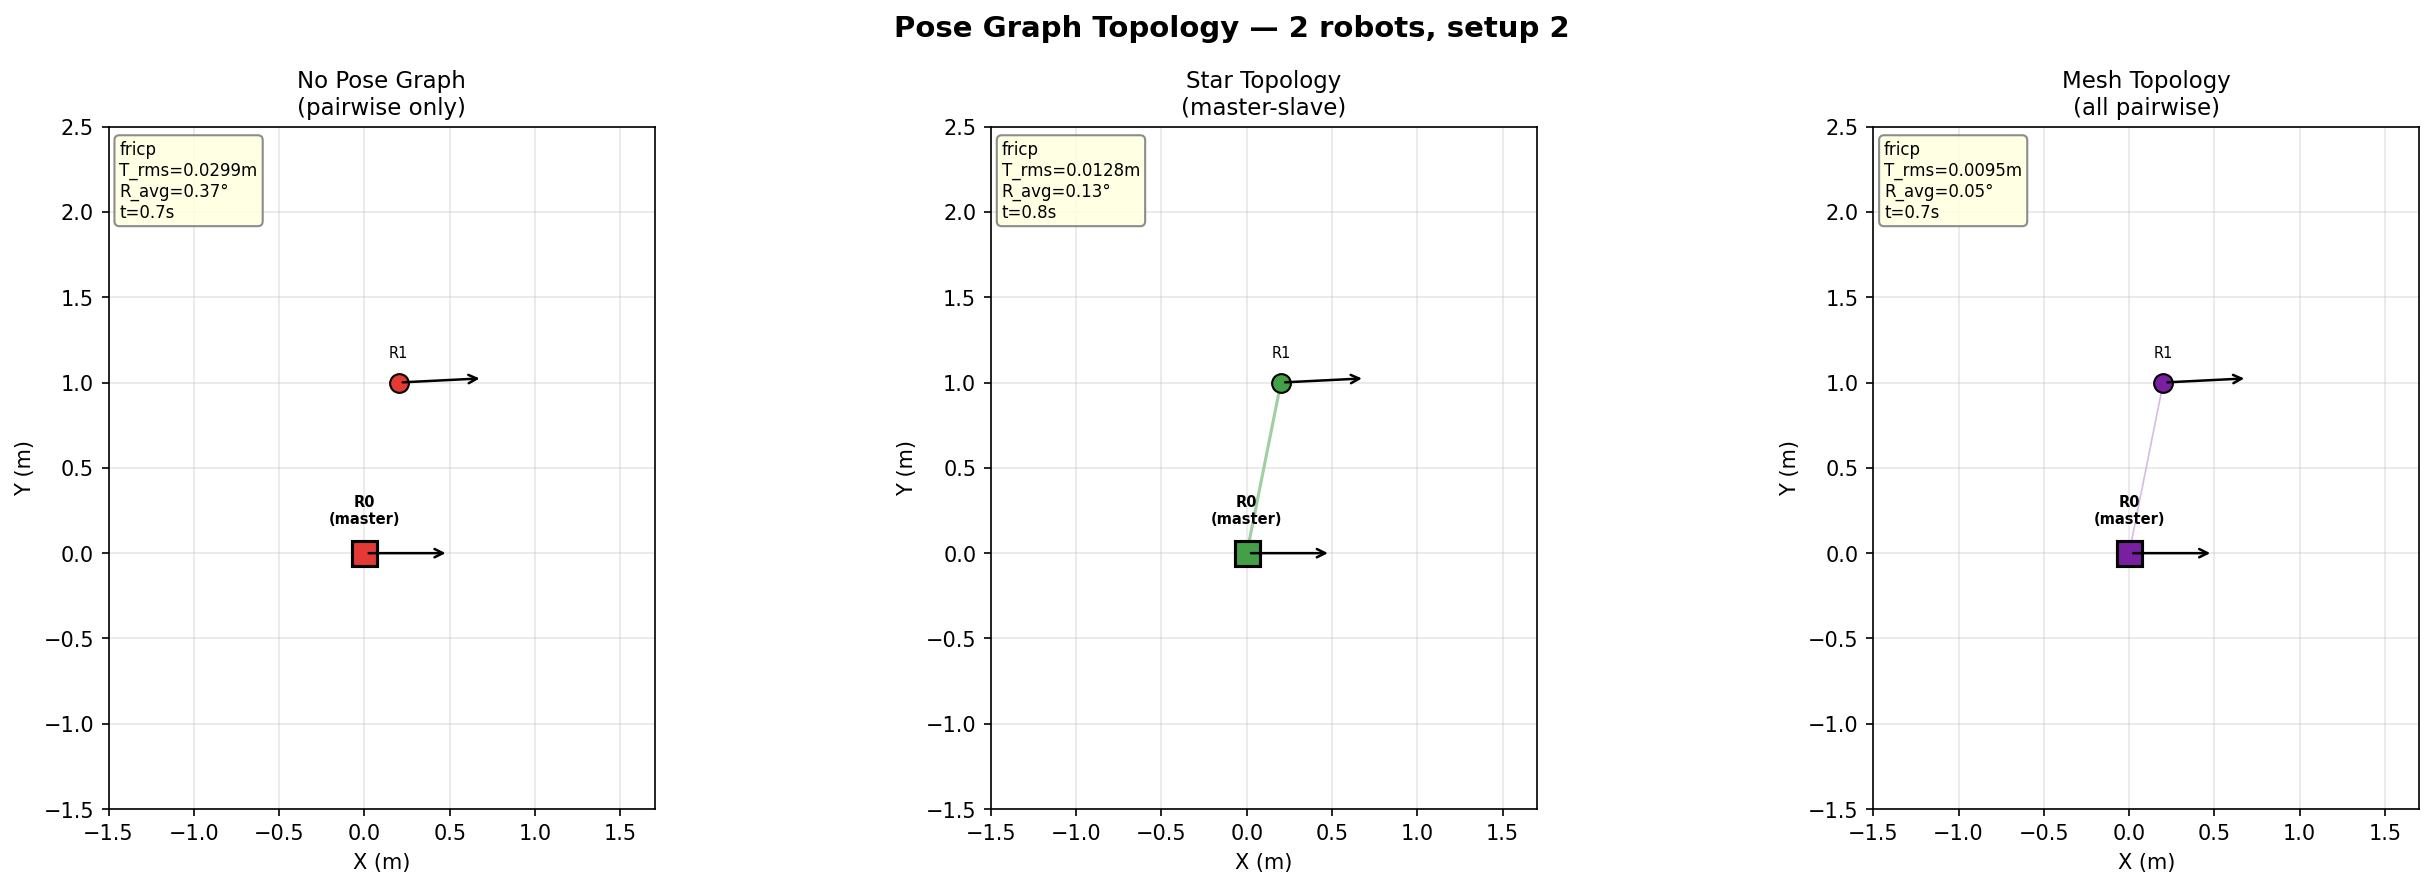
\includegraphics[width=0.7\textwidth]{figures/robots_2_setup_2_pose_graph.png}
    \caption{Pose graph visualization --- 2~robots, Setup~2.}
    \label{fig:app_2r_s2_pg}
\end{figure}

\begin{figure}[htbp]
    \centering
    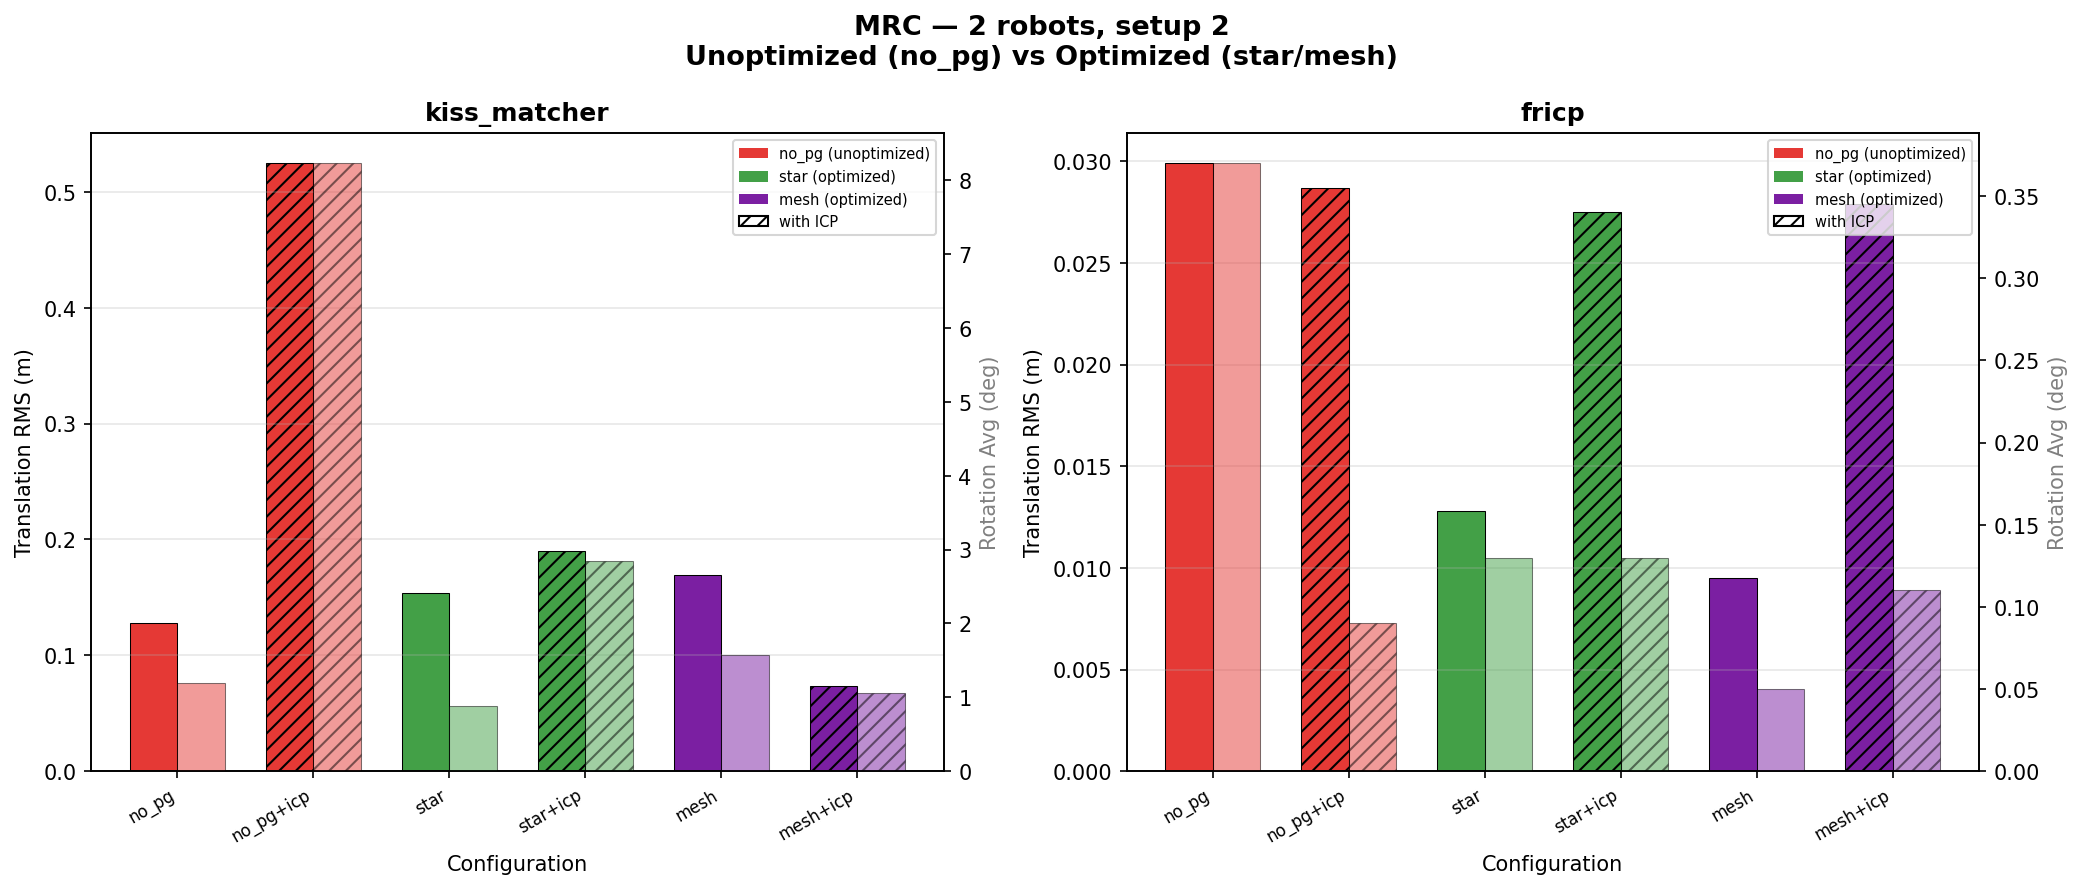
\includegraphics[width=0.95\textwidth]{figures/robots_2_setup_2_unopt_vs_opt.png}
    \caption{Unoptimized vs.\ optimized comparison --- 2~robots, Setup~2.}
    \label{fig:app_2r_s2_unopt}
\end{figure}

%% --- Setup 3 ---
\subsection{Setup~3: Behind + Small Yaw}

\begin{table}[htbp]
    \centering
    \caption{2~robots, Setup~3 --- behind at \SI{2.0}{\metre}
             with $\Delta\psi = -4.6\degree$
             (overlap: 64.2\%).}
    \label{tab:app_2r_s3}
    \small
    \begin{tabular}{l r r r r}
        \toprule
        \textbf{Configuration}
            & $\bar{e}_t$ [mm]
            & $\bar{e}_r$ [deg]
            & Ovlp [\%]
            & $t$ [s] \\
        \midrule
        \multicolumn{5}{l}{\textit{KISS-Matcher}} \\
        \quad no PG         & 144.8 & 1.08 & 64.2 & 0.1 \\
        \quad star PG       & 181.1 & 2.18 & 64.2 & 0.1 \\
        \quad mesh PG       & 277.3 & 3.32 & 64.2 & 0.1 \\
        \quad no PG + ICP   & 107.1 & 1.32 & 64.2 & 0.7 \\
        \quad star PG + ICP &  53.1 & 0.52 & 64.2 & 0.7 \\
        \quad mesh PG + ICP &  31.7 & 0.29 & 64.2 & 0.7 \\
        \midrule
        \multicolumn{5}{l}{\textit{FRICP}} \\
        \quad no PG         &  14.2 & 0.11 & 64.2 & 0.9 \\
        \quad star PG       &   6.0 & 0.04 & 64.2 & 0.8 \\
        \quad mesh PG       &   5.1 & 0.02 & 64.2 & 0.8 \\
        \quad no PG + ICP   &  18.5 & 0.13 & 64.2 & 1.4 \\
        \quad star PG + ICP &  29.4 & 0.11 & 64.2 & 1.4 \\
        \quad mesh PG + ICP &  29.3 & 0.13 & 64.2 & 1.3 \\
        \bottomrule
    \end{tabular}
\end{table}

\begin{figure}[htbp]
    \centering
    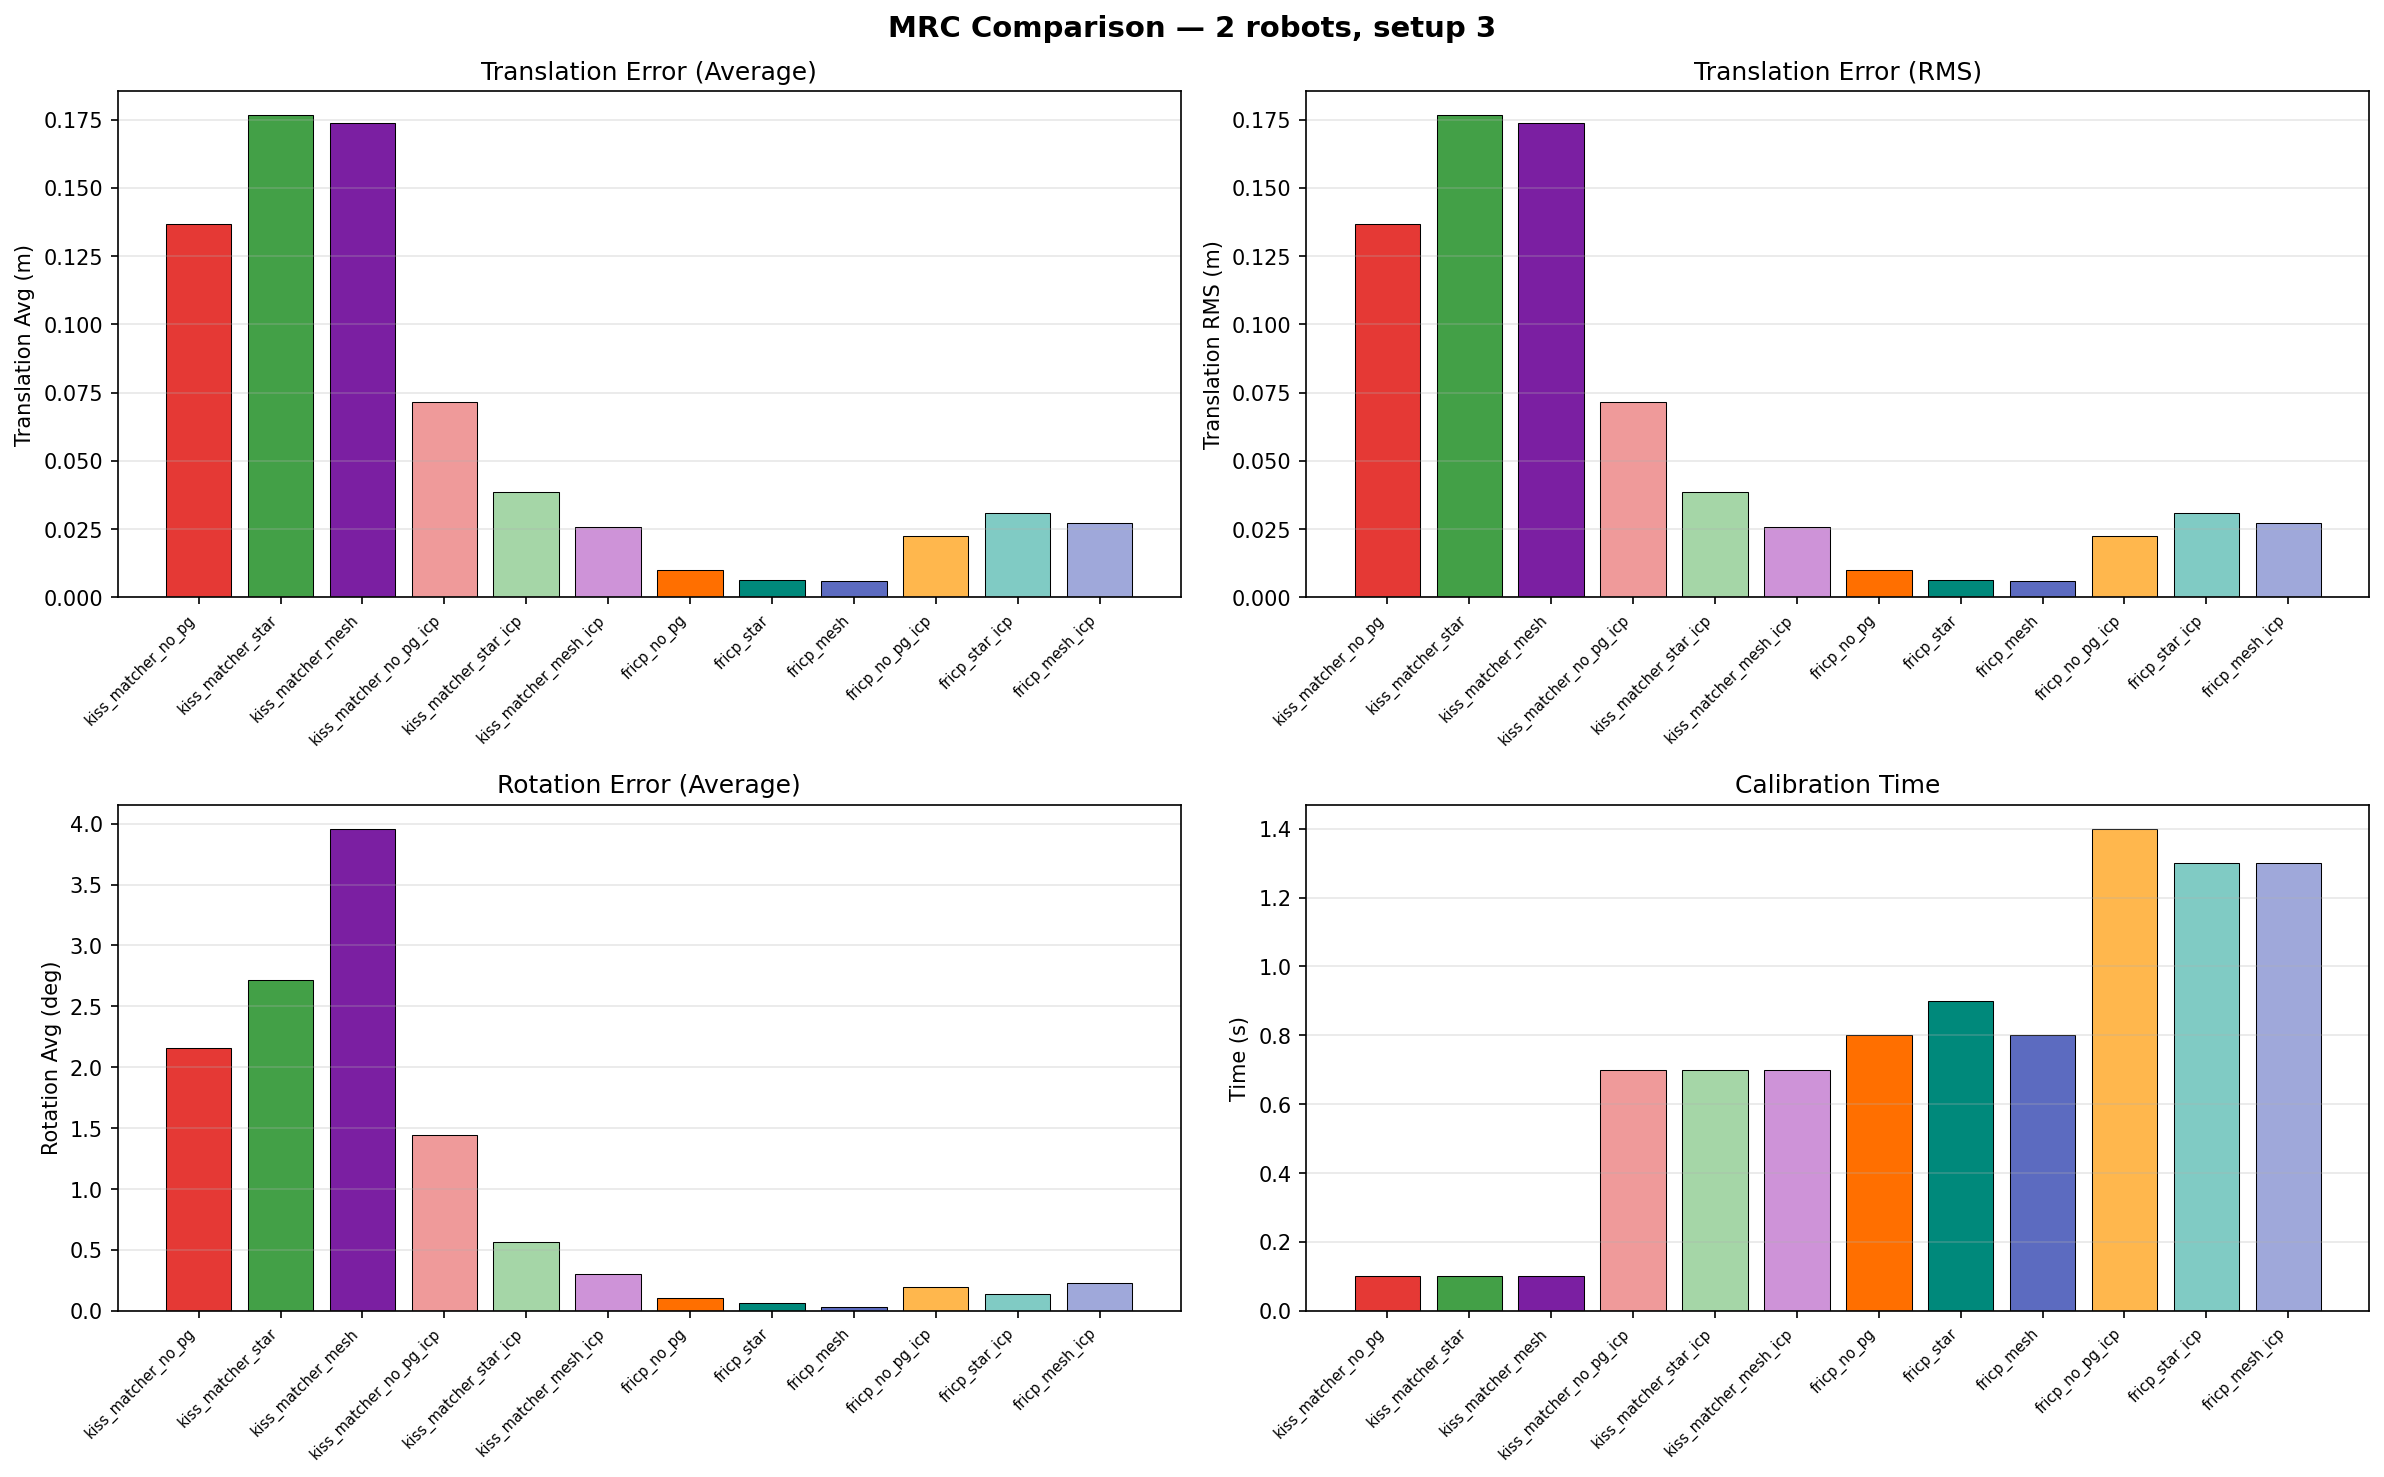
\includegraphics[width=0.95\textwidth]{figures/robots_2_setup_3_bars.png}
    \caption{Configuration comparison --- 2~robots, Setup~3.}
    \label{fig:app_2r_s3_bars}
\end{figure}

\begin{figure}[htbp]
    \centering
    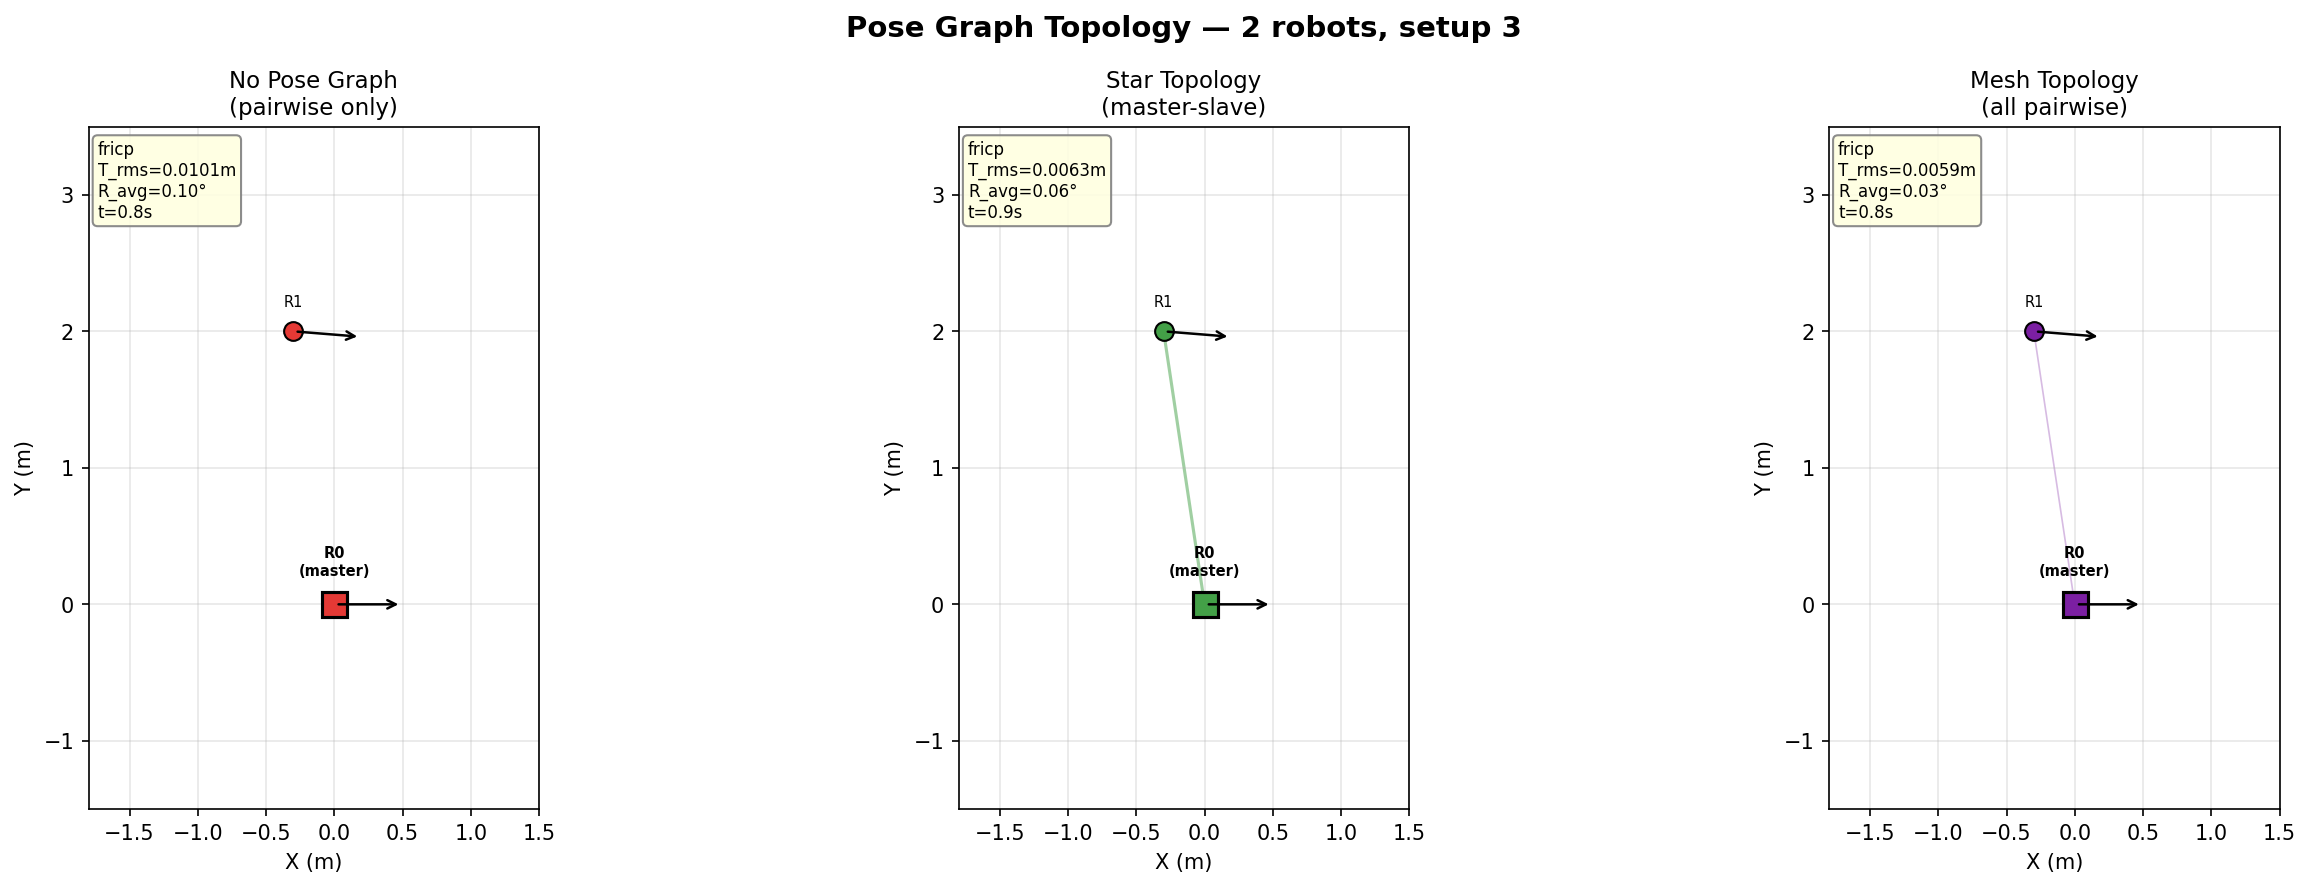
\includegraphics[width=0.7\textwidth]{figures/robots_2_setup_3_pose_graph.png}
    \caption{Pose graph visualization --- 2~robots, Setup~3.}
    \label{fig:app_2r_s3_pg}
\end{figure}

\begin{figure}[htbp]
    \centering
    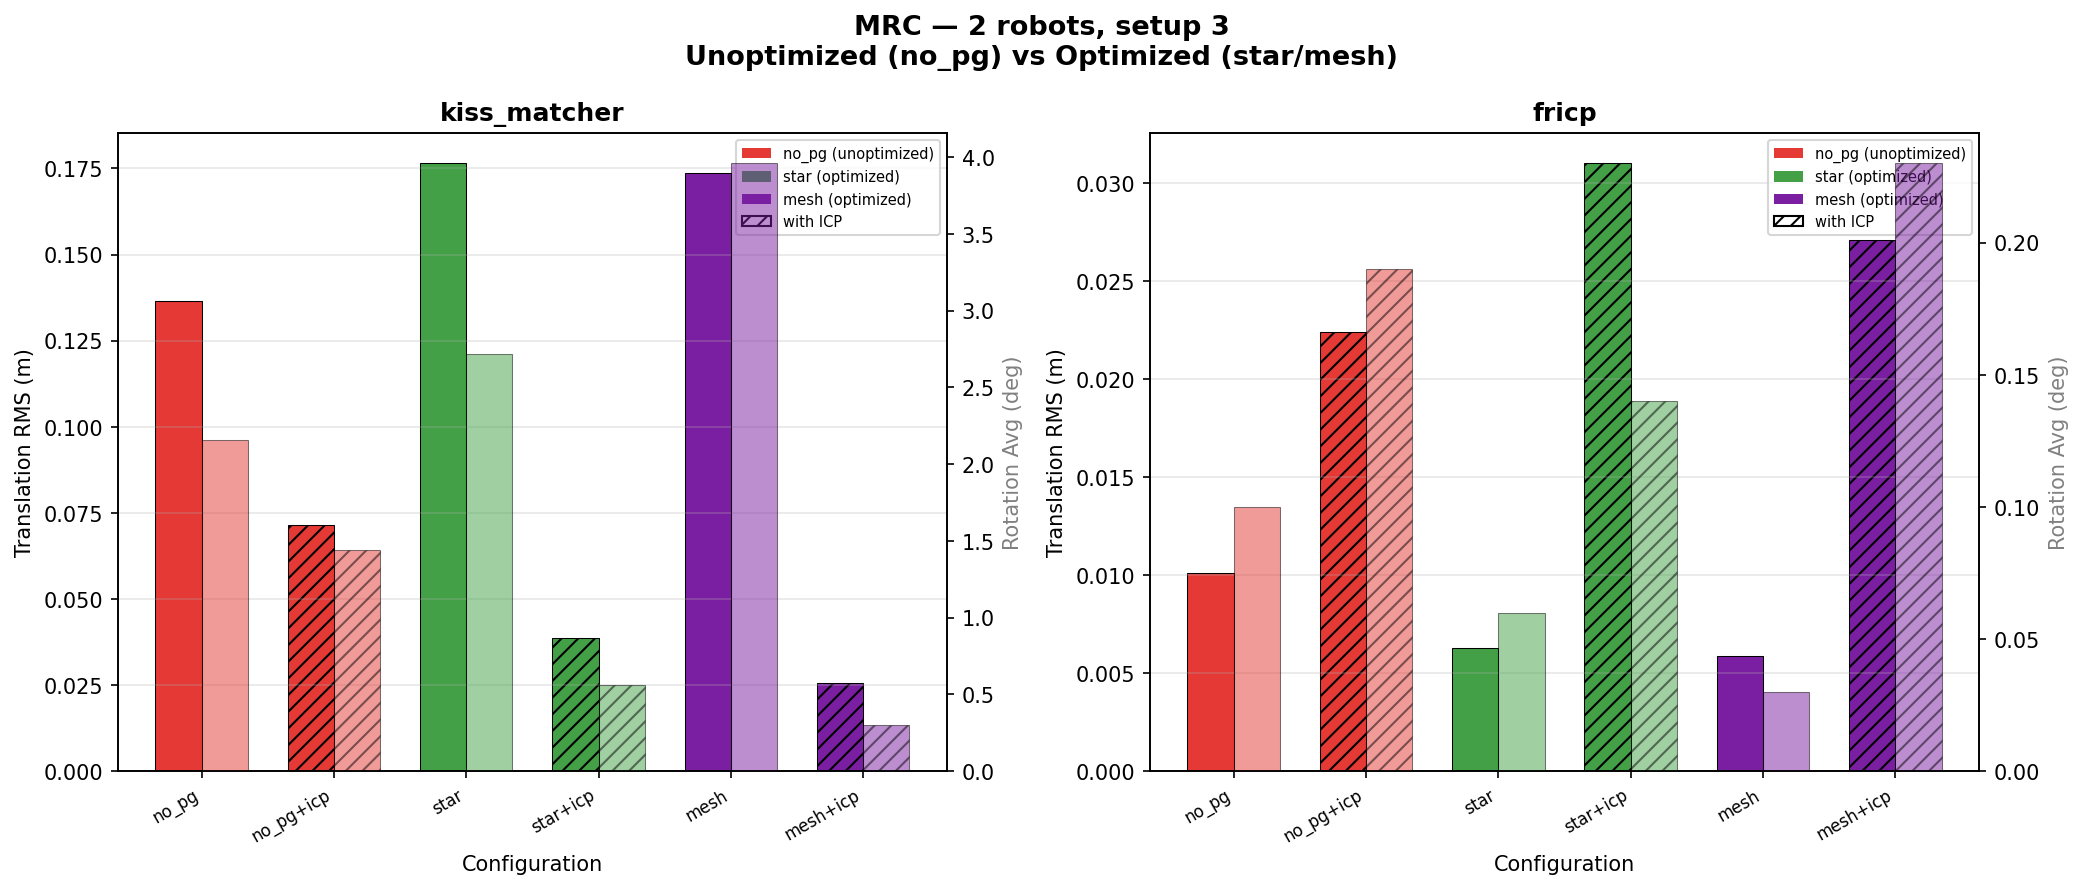
\includegraphics[width=0.95\textwidth]{figures/robots_2_setup_3_unopt_vs_opt.png}
    \caption{Unoptimized vs.\ optimized comparison --- 2~robots, Setup~3.}
    \label{fig:app_2r_s3_unopt}
\end{figure}

%% --- Setup 4 ---
\subsection{Setup~4: Both with Yaw Noise}

\begin{table}[htbp]
    \centering
    \caption{2~robots, Setup~4 --- yaw noise at \SI{1.2}{\metre}
             with $\Delta\psi = -4.6\degree$
             (overlap: 65.0\%).}
    \label{tab:app_2r_s4}
    \small
    \begin{tabular}{l r r r r}
        \toprule
        \textbf{Configuration}
            & $\bar{e}_t$ [mm]
            & $\bar{e}_r$ [deg]
            & Ovlp [\%]
            & $t$ [s] \\
        \midrule
        \multicolumn{5}{l}{\textit{KISS-Matcher}} \\
        \quad no PG         & 221.6 & 2.51 & 65.0 & 0.1 \\
        \quad star PG       & 231.2 & 3.58 & 65.0 & 0.1 \\
        \quad mesh PG       & 213.1 & 3.12 & 65.0 & 0.1 \\
        \quad no PG + ICP   &  79.1 & 1.11 & 65.0 & 0.6 \\
        \quad star PG + ICP &  36.9 & 0.44 & 65.0 & 0.6 \\
        \quad mesh PG + ICP &  20.7 & 0.17 & 65.0 & 0.6 \\
        \midrule
        \multicolumn{5}{l}{\textit{FRICP}} \\
        \quad no PG         &  14.1 & 0.08 & 65.0 & 0.8 \\
        \quad star PG       &  12.0 & 0.05 & 65.0 & 0.7 \\
        \quad mesh PG       &   6.4 & 0.02 & 65.0 & 0.8 \\
        \quad no PG + ICP   &  13.8 & 0.13 & 65.0 & 1.3 \\
        \quad star PG + ICP &  21.8 & 0.17 & 65.0 & 1.3 \\
        \quad mesh PG + ICP &  27.8 & 0.16 & 65.0 & 1.3 \\
        \bottomrule
    \end{tabular}
\end{table}

\begin{figure}[htbp]
    \centering
    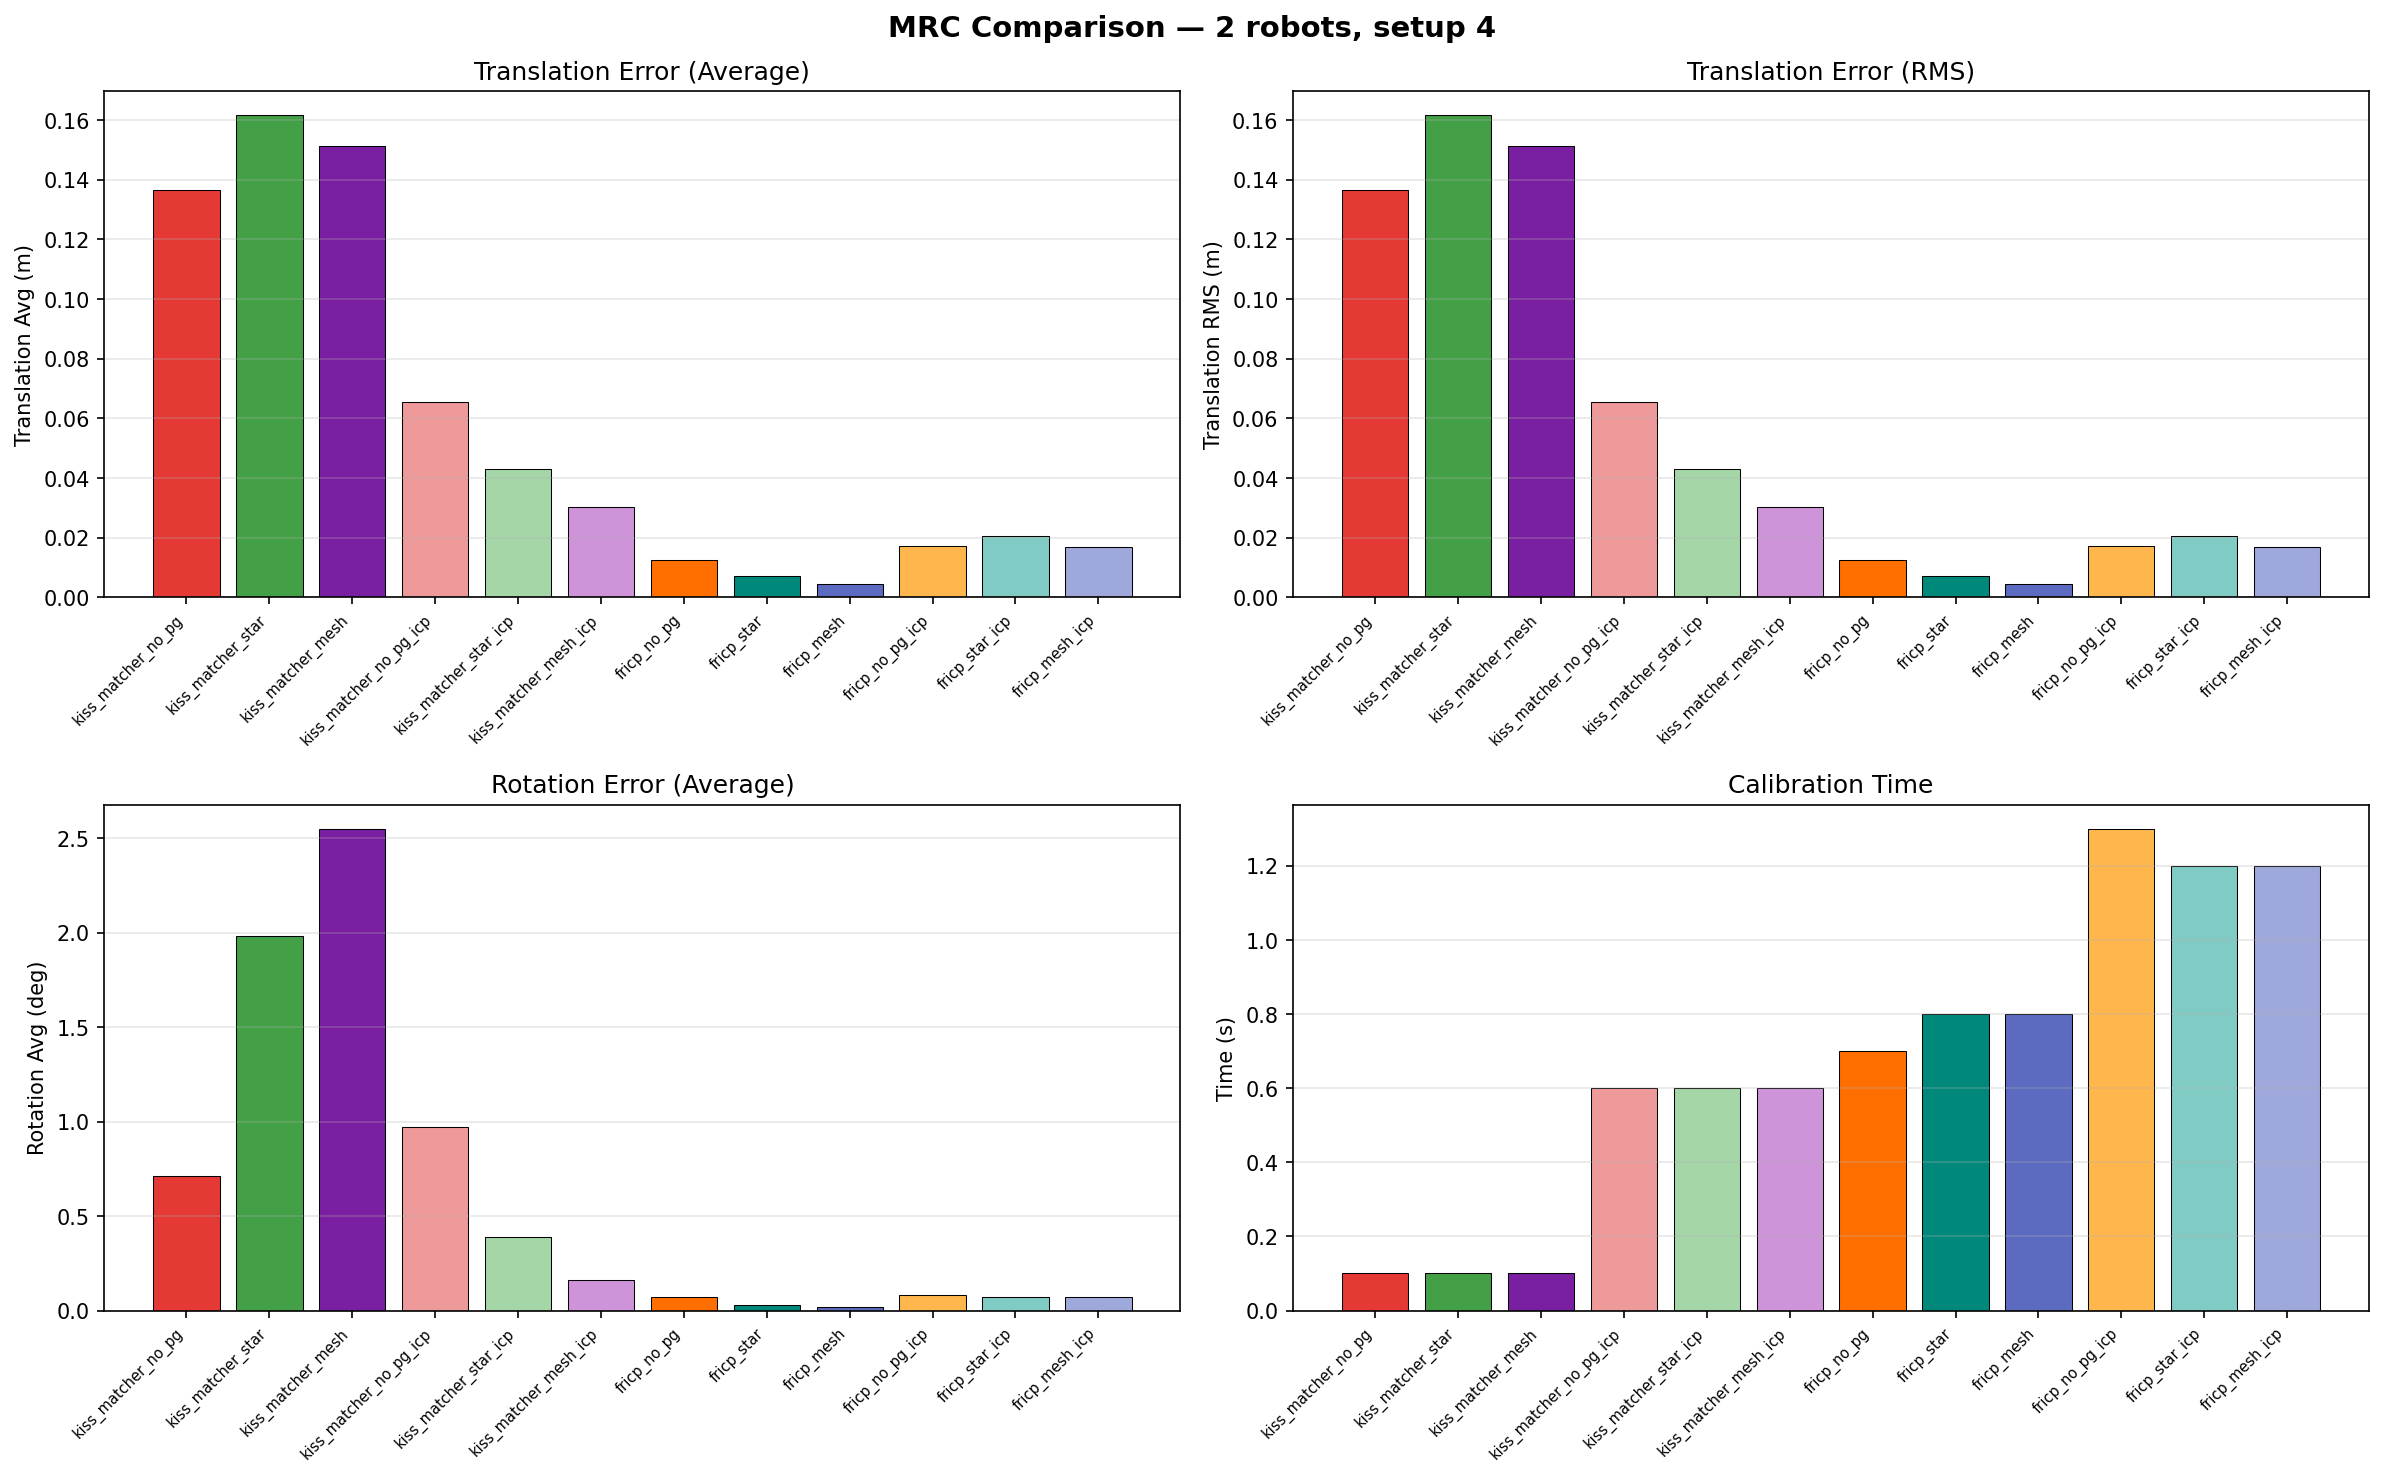
\includegraphics[width=0.95\textwidth]{figures/robots_2_setup_4_bars.png}
    \caption{Configuration comparison --- 2~robots, Setup~4.}
    \label{fig:app_2r_s4_bars}
\end{figure}

\begin{figure}[htbp]
    \centering
    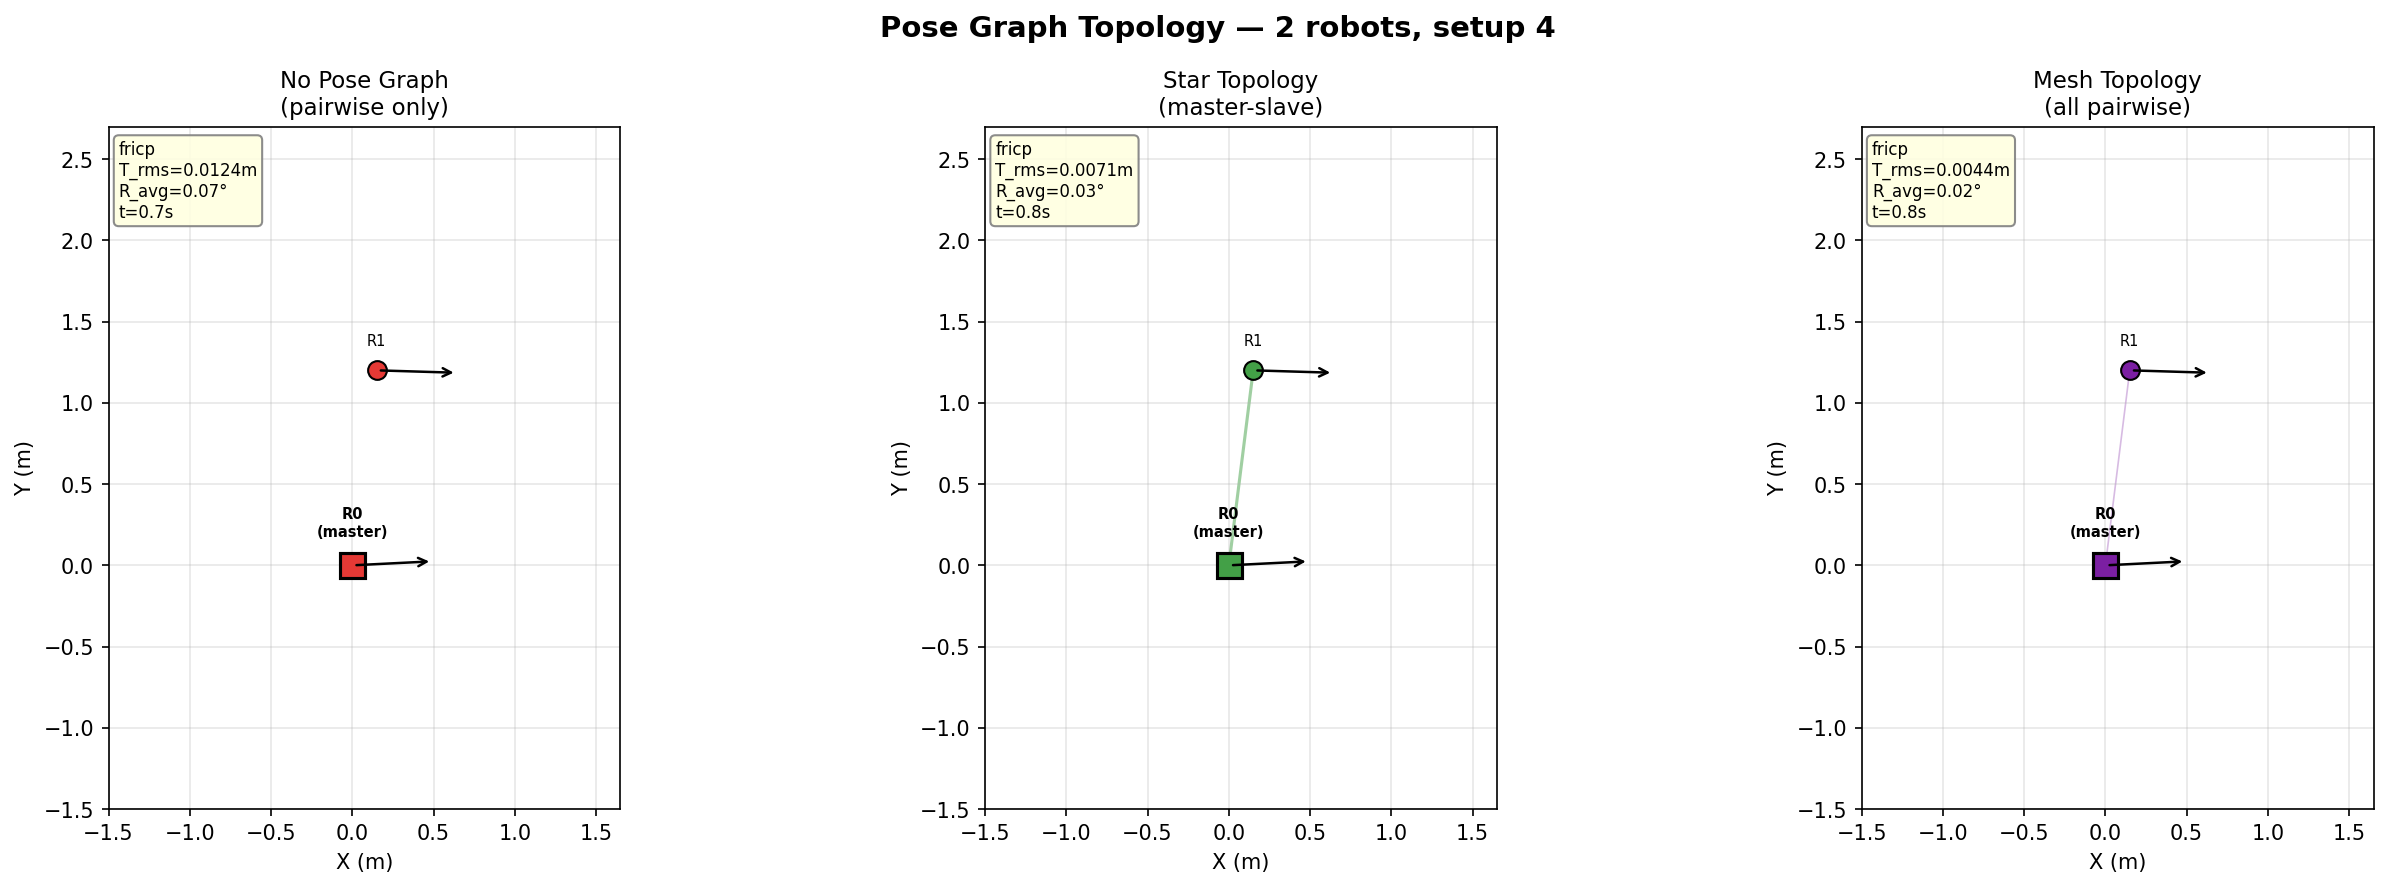
\includegraphics[width=0.7\textwidth]{figures/robots_2_setup_4_pose_graph.png}
    \caption{Pose graph visualization --- 2~robots, Setup~4.}
    \label{fig:app_2r_s4_pg}
\end{figure}

\begin{figure}[htbp]
    \centering
    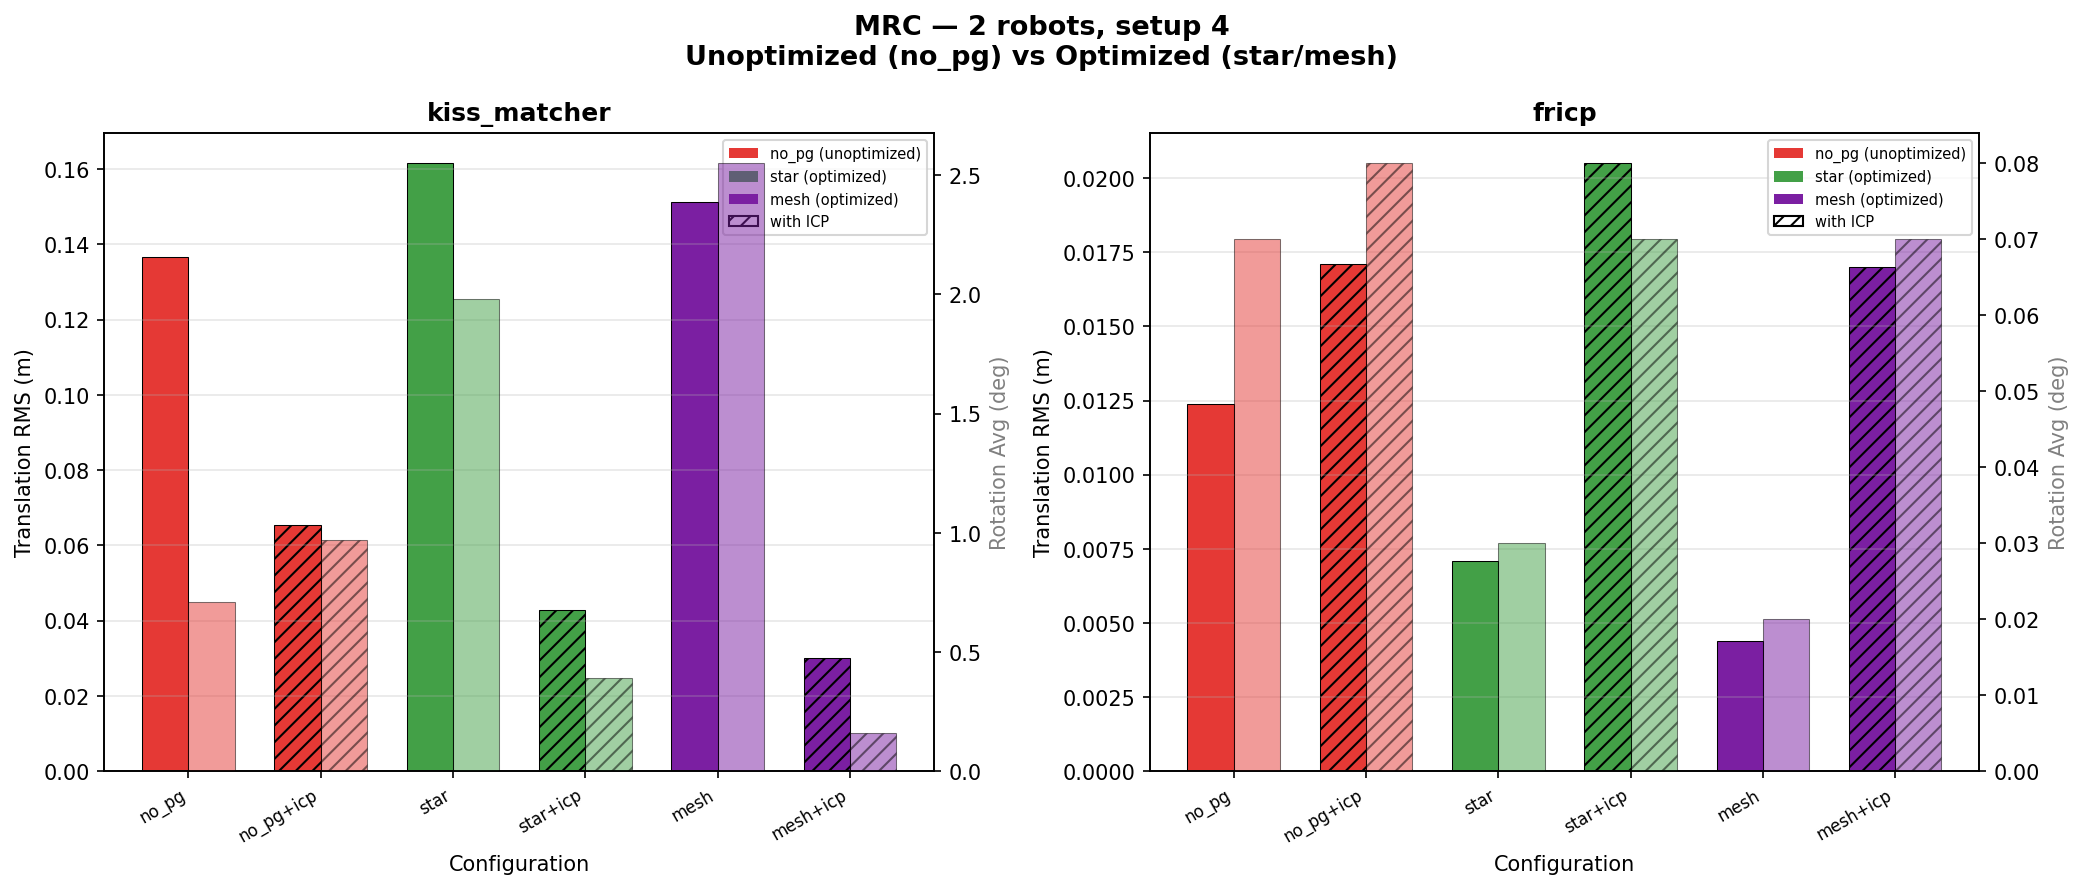
\includegraphics[width=0.95\textwidth]{figures/robots_2_setup_4_unopt_vs_opt.png}
    \caption{Unoptimized vs.\ optimized comparison --- 2~robots, Setup~4.}
    \label{fig:app_2r_s4_unopt}
\end{figure}

%% --- Setup 5 ---
\subsection{Setup~5: Very Close, More Noise}

\begin{table}[htbp]
    \centering
    \caption{2~robots, Setup~5 --- very close at \SI{0.8}{\metre}
             with $\Delta\psi = 5.7\degree$
             (overlap: 70.9\%).}
    \label{tab:app_2r_s5}
    \small
    \begin{tabular}{l r r r r}
        \toprule
        \textbf{Configuration}
            & $\bar{e}_t$ [mm]
            & $\bar{e}_r$ [deg]
            & Ovlp [\%]
            & $t$ [s] \\
        \midrule
        \multicolumn{5}{l}{\textit{KISS-Matcher}} \\
        \quad no PG         &  37.1 & 1.74 & 70.9 & 0.1 \\
        \quad star PG       &  94.6 & 1.57 & 70.9 & 0.1 \\
        \quad mesh PG       & 103.4 & 2.68 & 70.9 & 0.1 \\
        \quad no PG + ICP   &  60.8 & 1.10 & 70.9 & 0.6 \\
        \quad star PG + ICP &  37.8 & 0.50 & 70.9 & 0.6 \\
        \quad mesh PG + ICP &  20.9 & 0.27 & 70.9 & 0.6 \\
        \midrule
        \multicolumn{5}{l}{\textit{FRICP}} \\
        \quad no PG         &   8.7 & 0.11 & 70.9 & 0.7 \\
        \quad star PG       &   5.8 & 0.05 & 70.9 & 0.8 \\
        \quad mesh PG       &   5.5 & 0.03 & 70.9 & 0.7 \\
        \quad no PG + ICP   &  17.7 & 0.13 & 70.9 & 1.2 \\
        \quad star PG + ICP &  24.0 & 0.23 & 70.9 & 1.3 \\
        \quad mesh PG + ICP &  20.3 & 0.16 & 70.9 & 1.2 \\
        \bottomrule
    \end{tabular}
\end{table}

\begin{figure}[htbp]
    \centering
    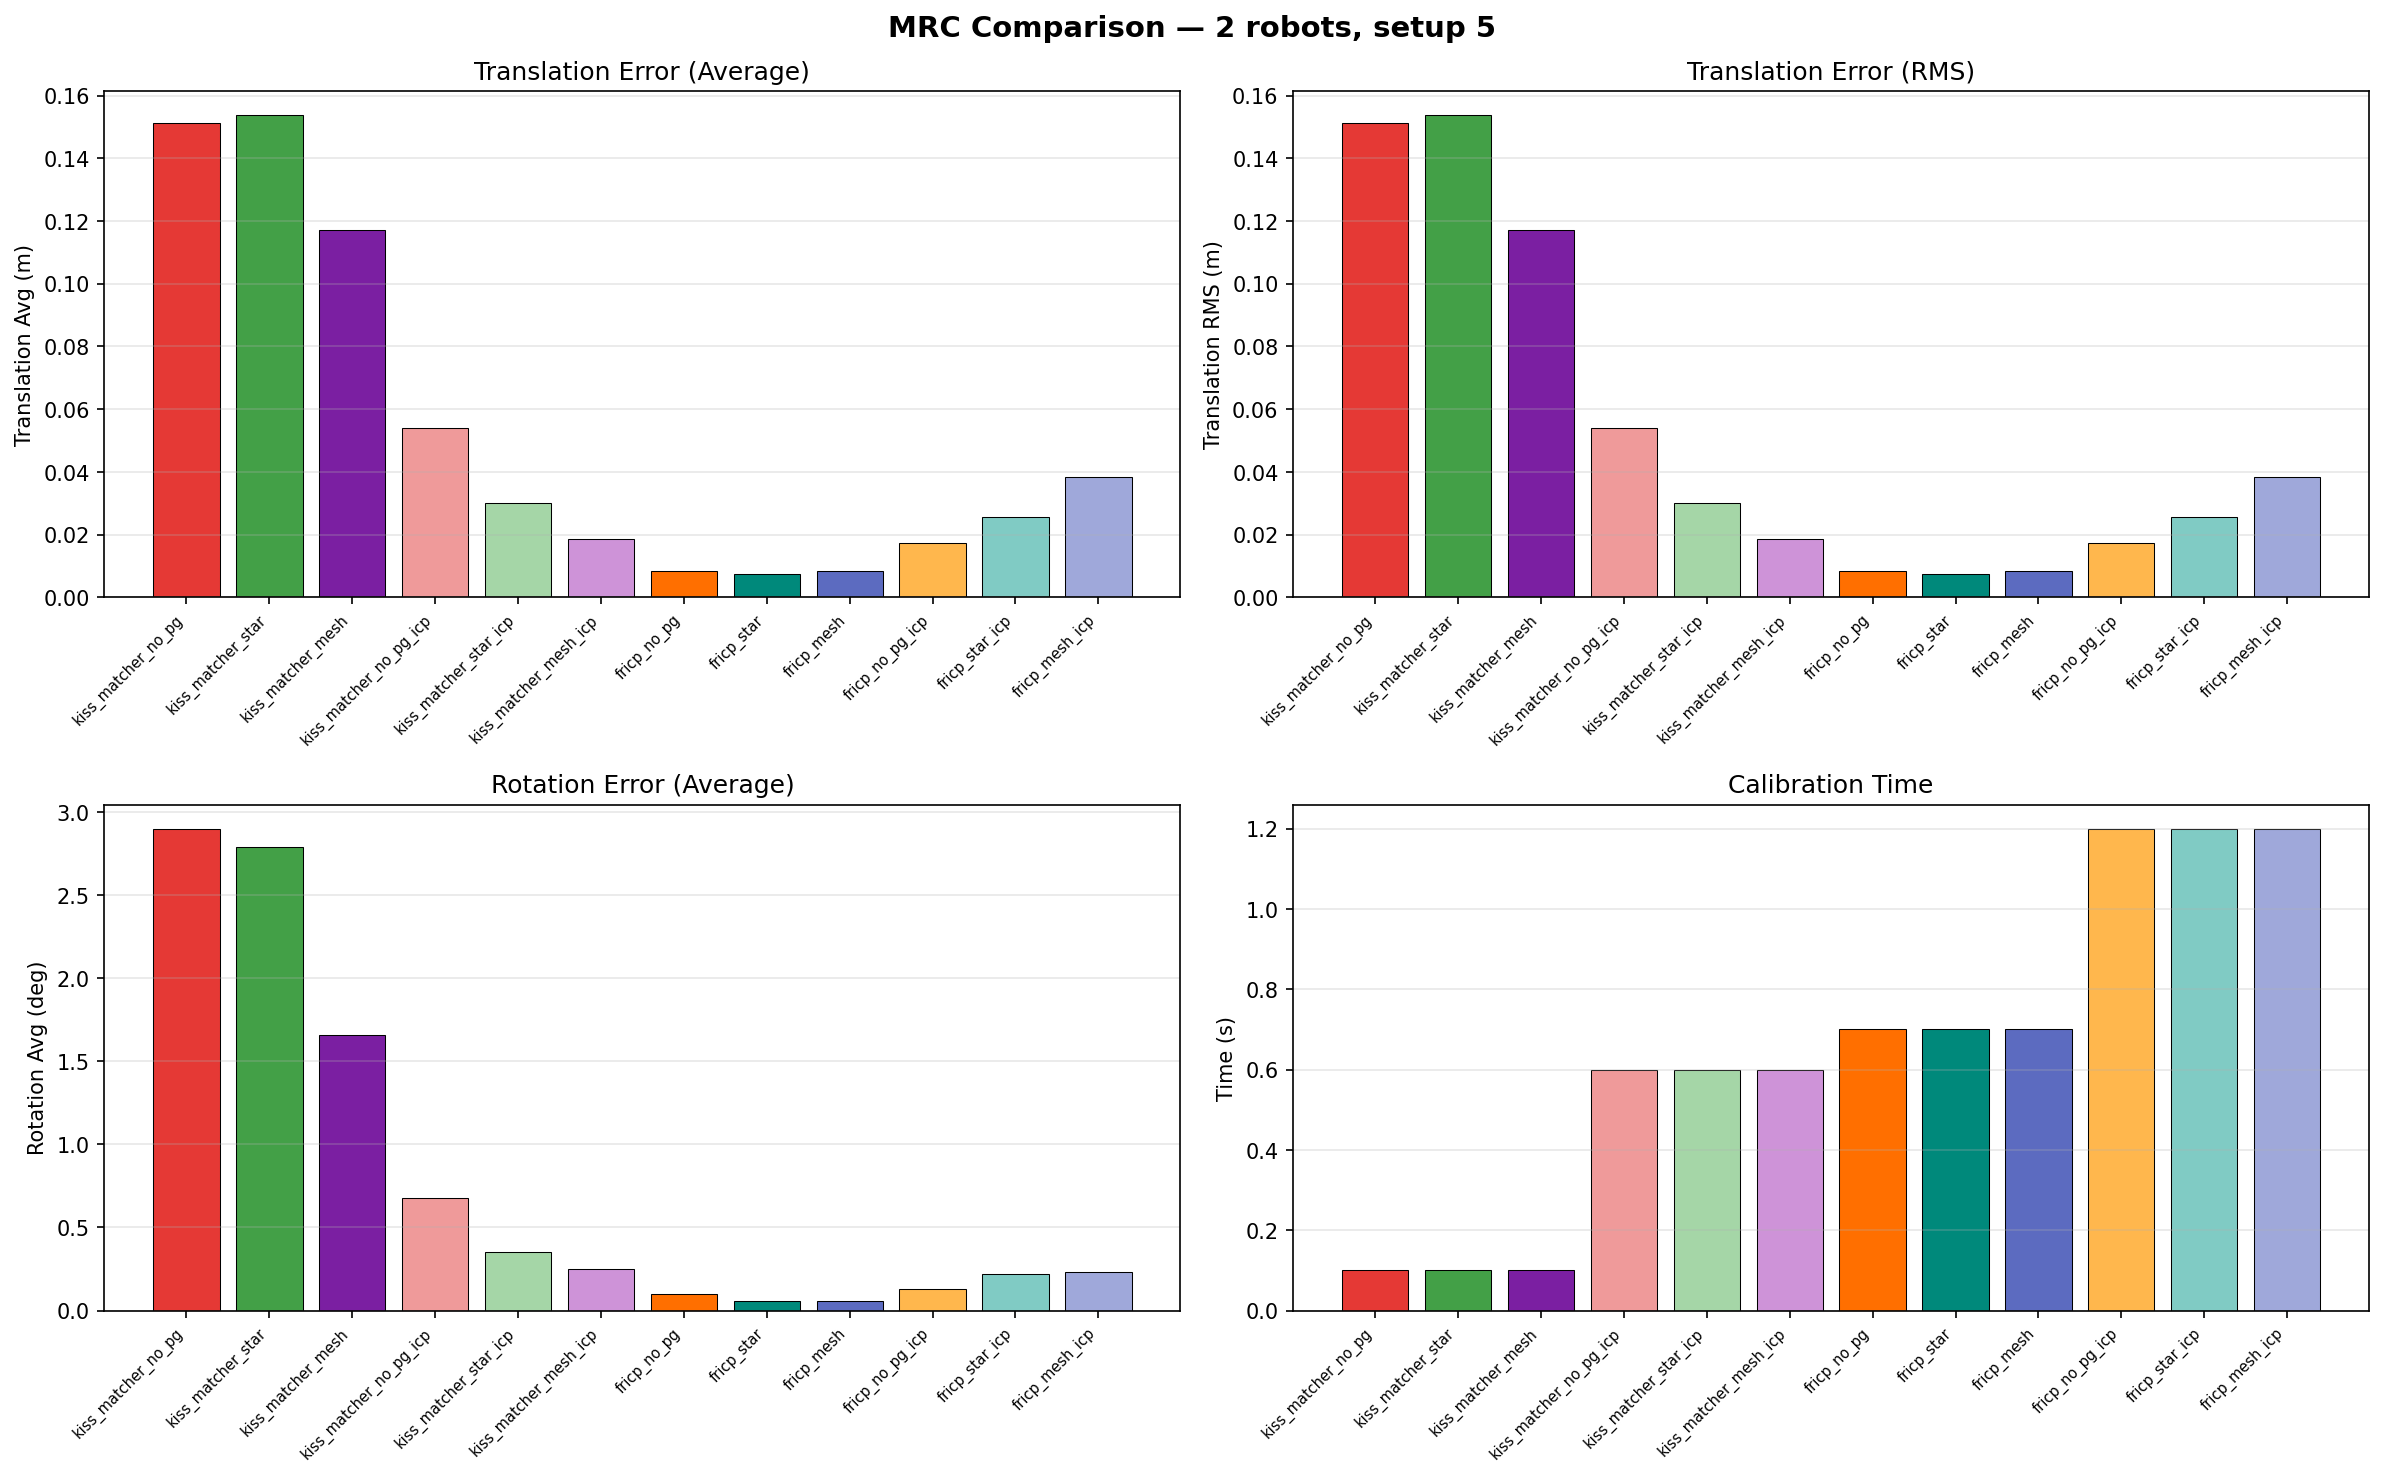
\includegraphics[width=0.95\textwidth]{figures/robots_2_setup_5_bars.png}
    \caption{Configuration comparison --- 2~robots, Setup~5.}
    \label{fig:app_2r_s5_bars}
\end{figure}

\begin{figure}[htbp]
    \centering
    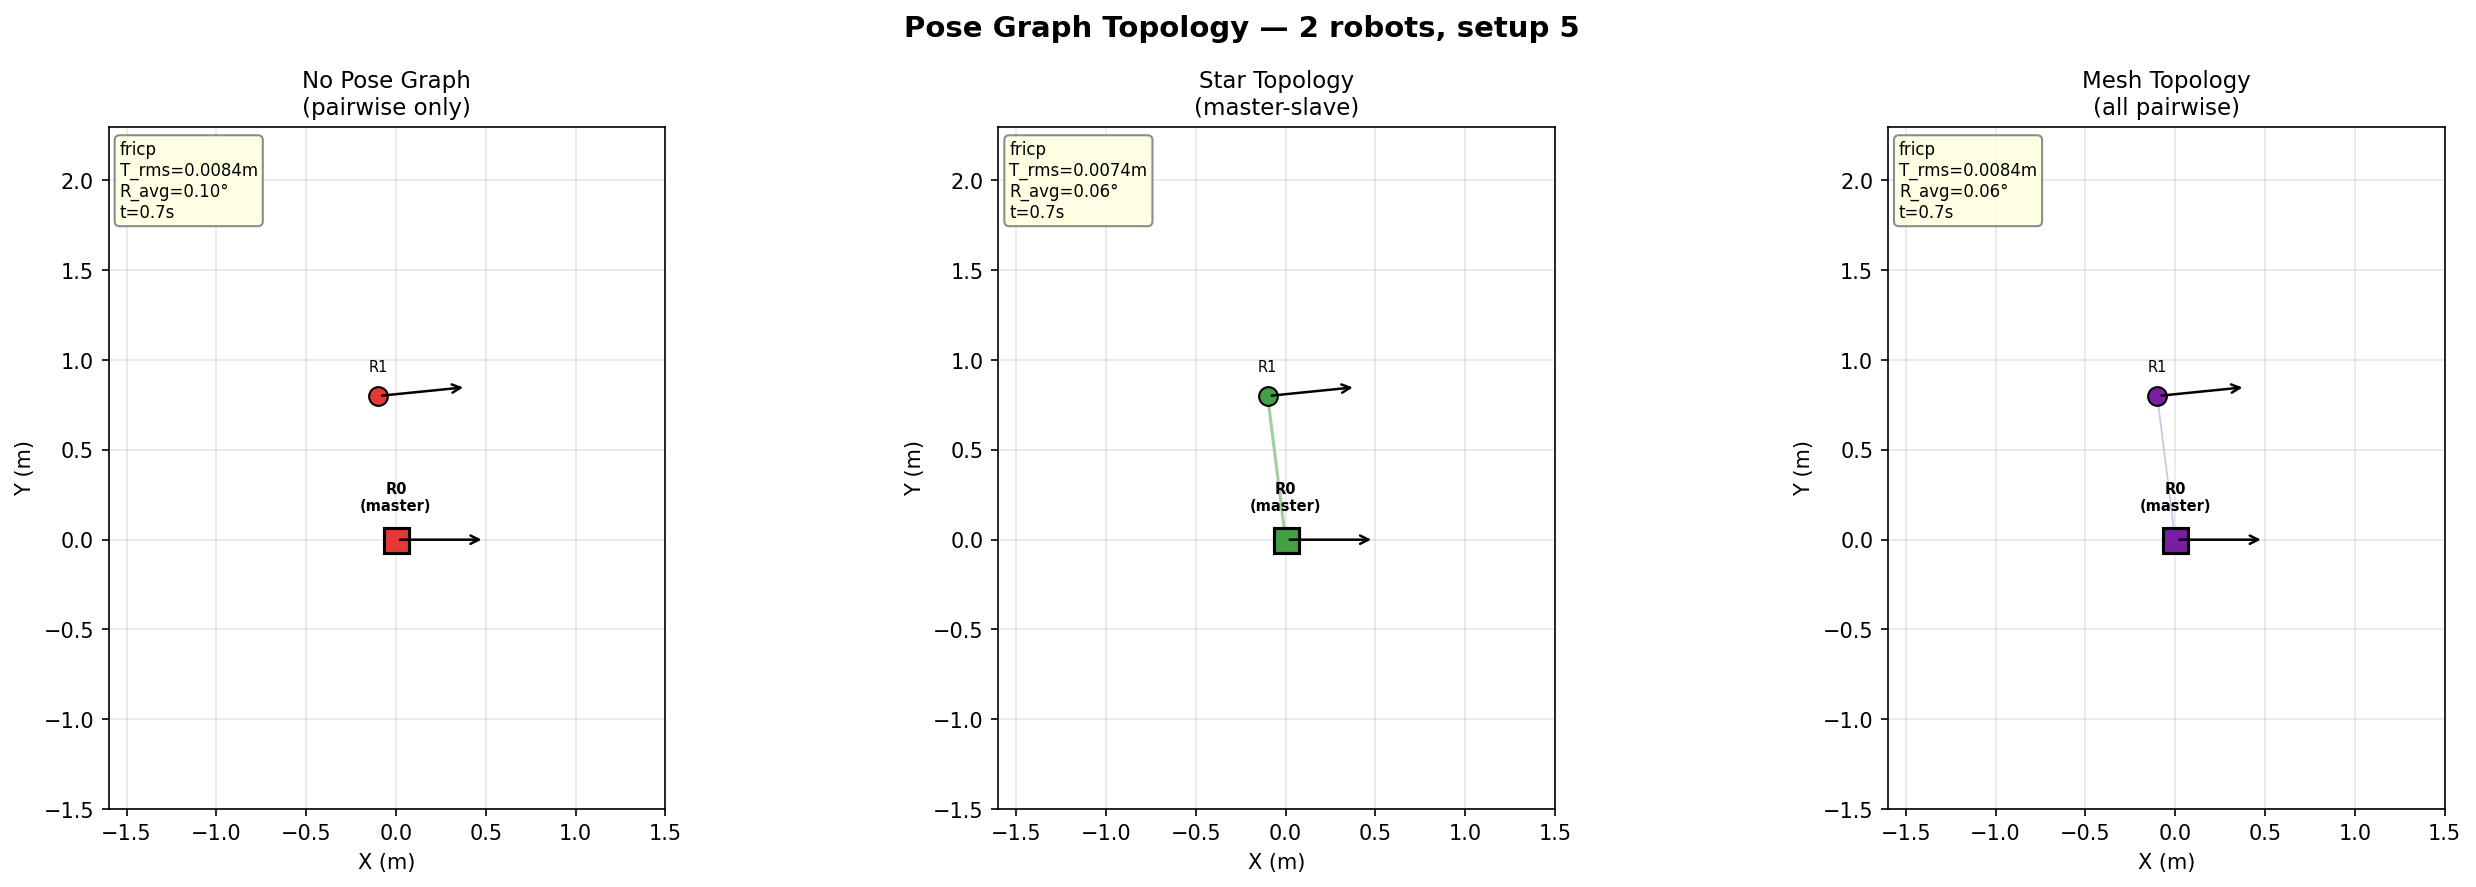
\includegraphics[width=0.7\textwidth]{figures/robots_2_setup_5_pose_graph.png}
    \caption{Pose graph visualization --- 2~robots, Setup~5.}
    \label{fig:app_2r_s5_pg}
\end{figure}

\begin{figure}[htbp]
    \centering
    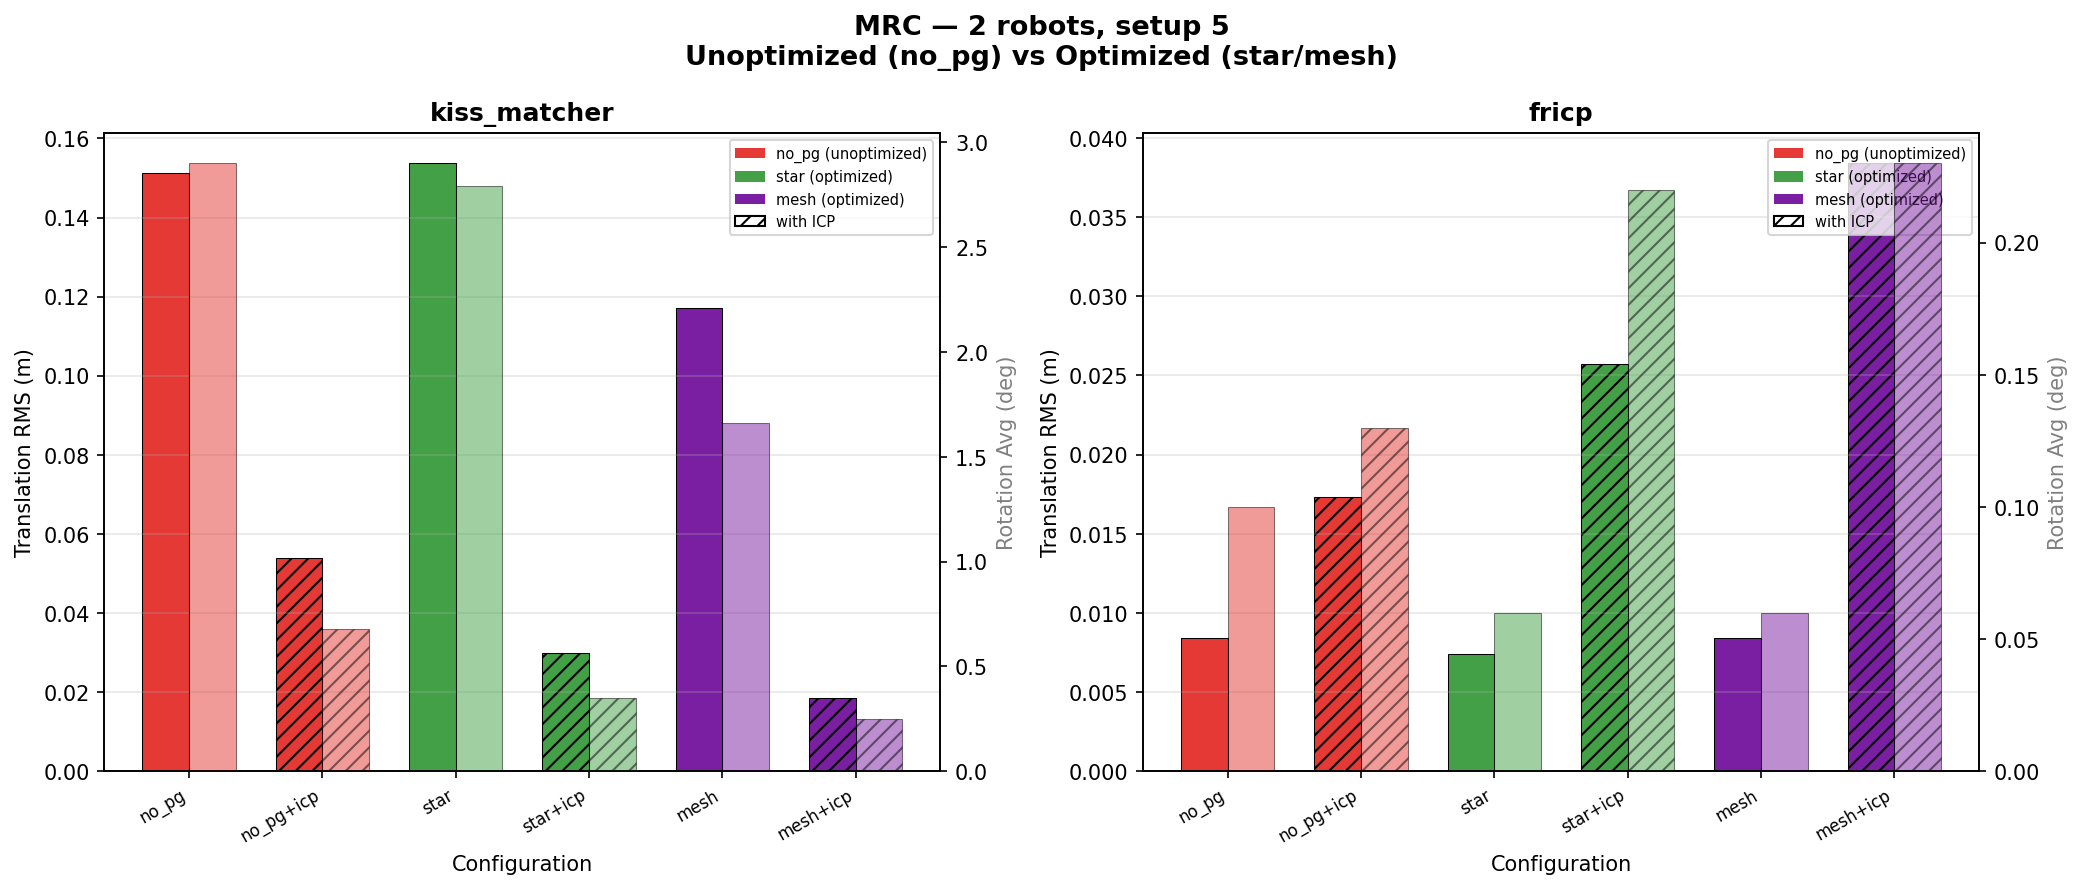
\includegraphics[width=0.95\textwidth]{figures/robots_2_setup_5_unopt_vs_opt.png}
    \caption{Unoptimized vs.\ optimized comparison --- 2~robots, Setup~5.}
    \label{fig:app_2r_s5_unopt}
\end{figure}

%% --- 2-robot averaged ---
\subsection{Averaged Results (2~Robots, Proximity)}

Results averaged over Setups~2--5 only (Setup~1 excluded due to
simulation anomaly).

\begin{table}[htbp]
    \centering
    \caption{2~robots proximity --- averaged over Setups~2--5
             (3 trials per configuration, overlap: 67.3\%).}
    \label{tab:app_2r_avg}
    \small
    \begin{tabular}{l r r r r}
        \toprule
        \textbf{Configuration}
            & $\bar{e}_t$ [mm]
            & $\bar{e}_r$ [deg]
            & Ovlp [\%]
            & $t$ [s] \\
        \midrule
        \multicolumn{5}{l}{\textit{KISS-Matcher}} \\
        \quad no PG         & 120.8  & 1.56  & 67.3 & 0.10 \\
        \quad star PG       & 153.8  & 2.08  & 67.3 & 0.10 \\
        \quad mesh PG       & 182.2  & 2.57  & 67.3 & 0.10 \\
        \quad no PG + ICP   &  76.3  & 1.02  & 67.3 & 0.63 \\
        \quad star PG + ICP &  43.0  & 0.44  & 67.3 & 0.63 \\
        \quad mesh PG + ICP &  26.4  & 0.24  & 67.3 & 0.63 \\
        \midrule
        \multicolumn{5}{l}{\textit{FRICP}} \\
        \quad no PG         &  13.0  & 0.10  & 67.3 & 0.78 \\
        \quad star PG       &   7.8  & 0.05  & 67.3 & 0.75 \\
        \quad mesh PG       & \textbf{5.4} & \textbf{0.03} & 67.3 & 0.78 \\
        \quad no PG + ICP   &  18.0  & 0.13  & 67.3 & 1.28 \\
        \quad star PG + ICP &  24.3  & 0.16  & 67.3 & 1.30 \\
        \quad mesh PG + ICP &  25.0  & 0.17  & 67.3 & 1.25 \\
        \bottomrule
    \end{tabular}
\end{table}

\subsection{Cross-Setup Summary (2~Robots, Proximity)}

\begin{figure}[htbp]
    \centering
    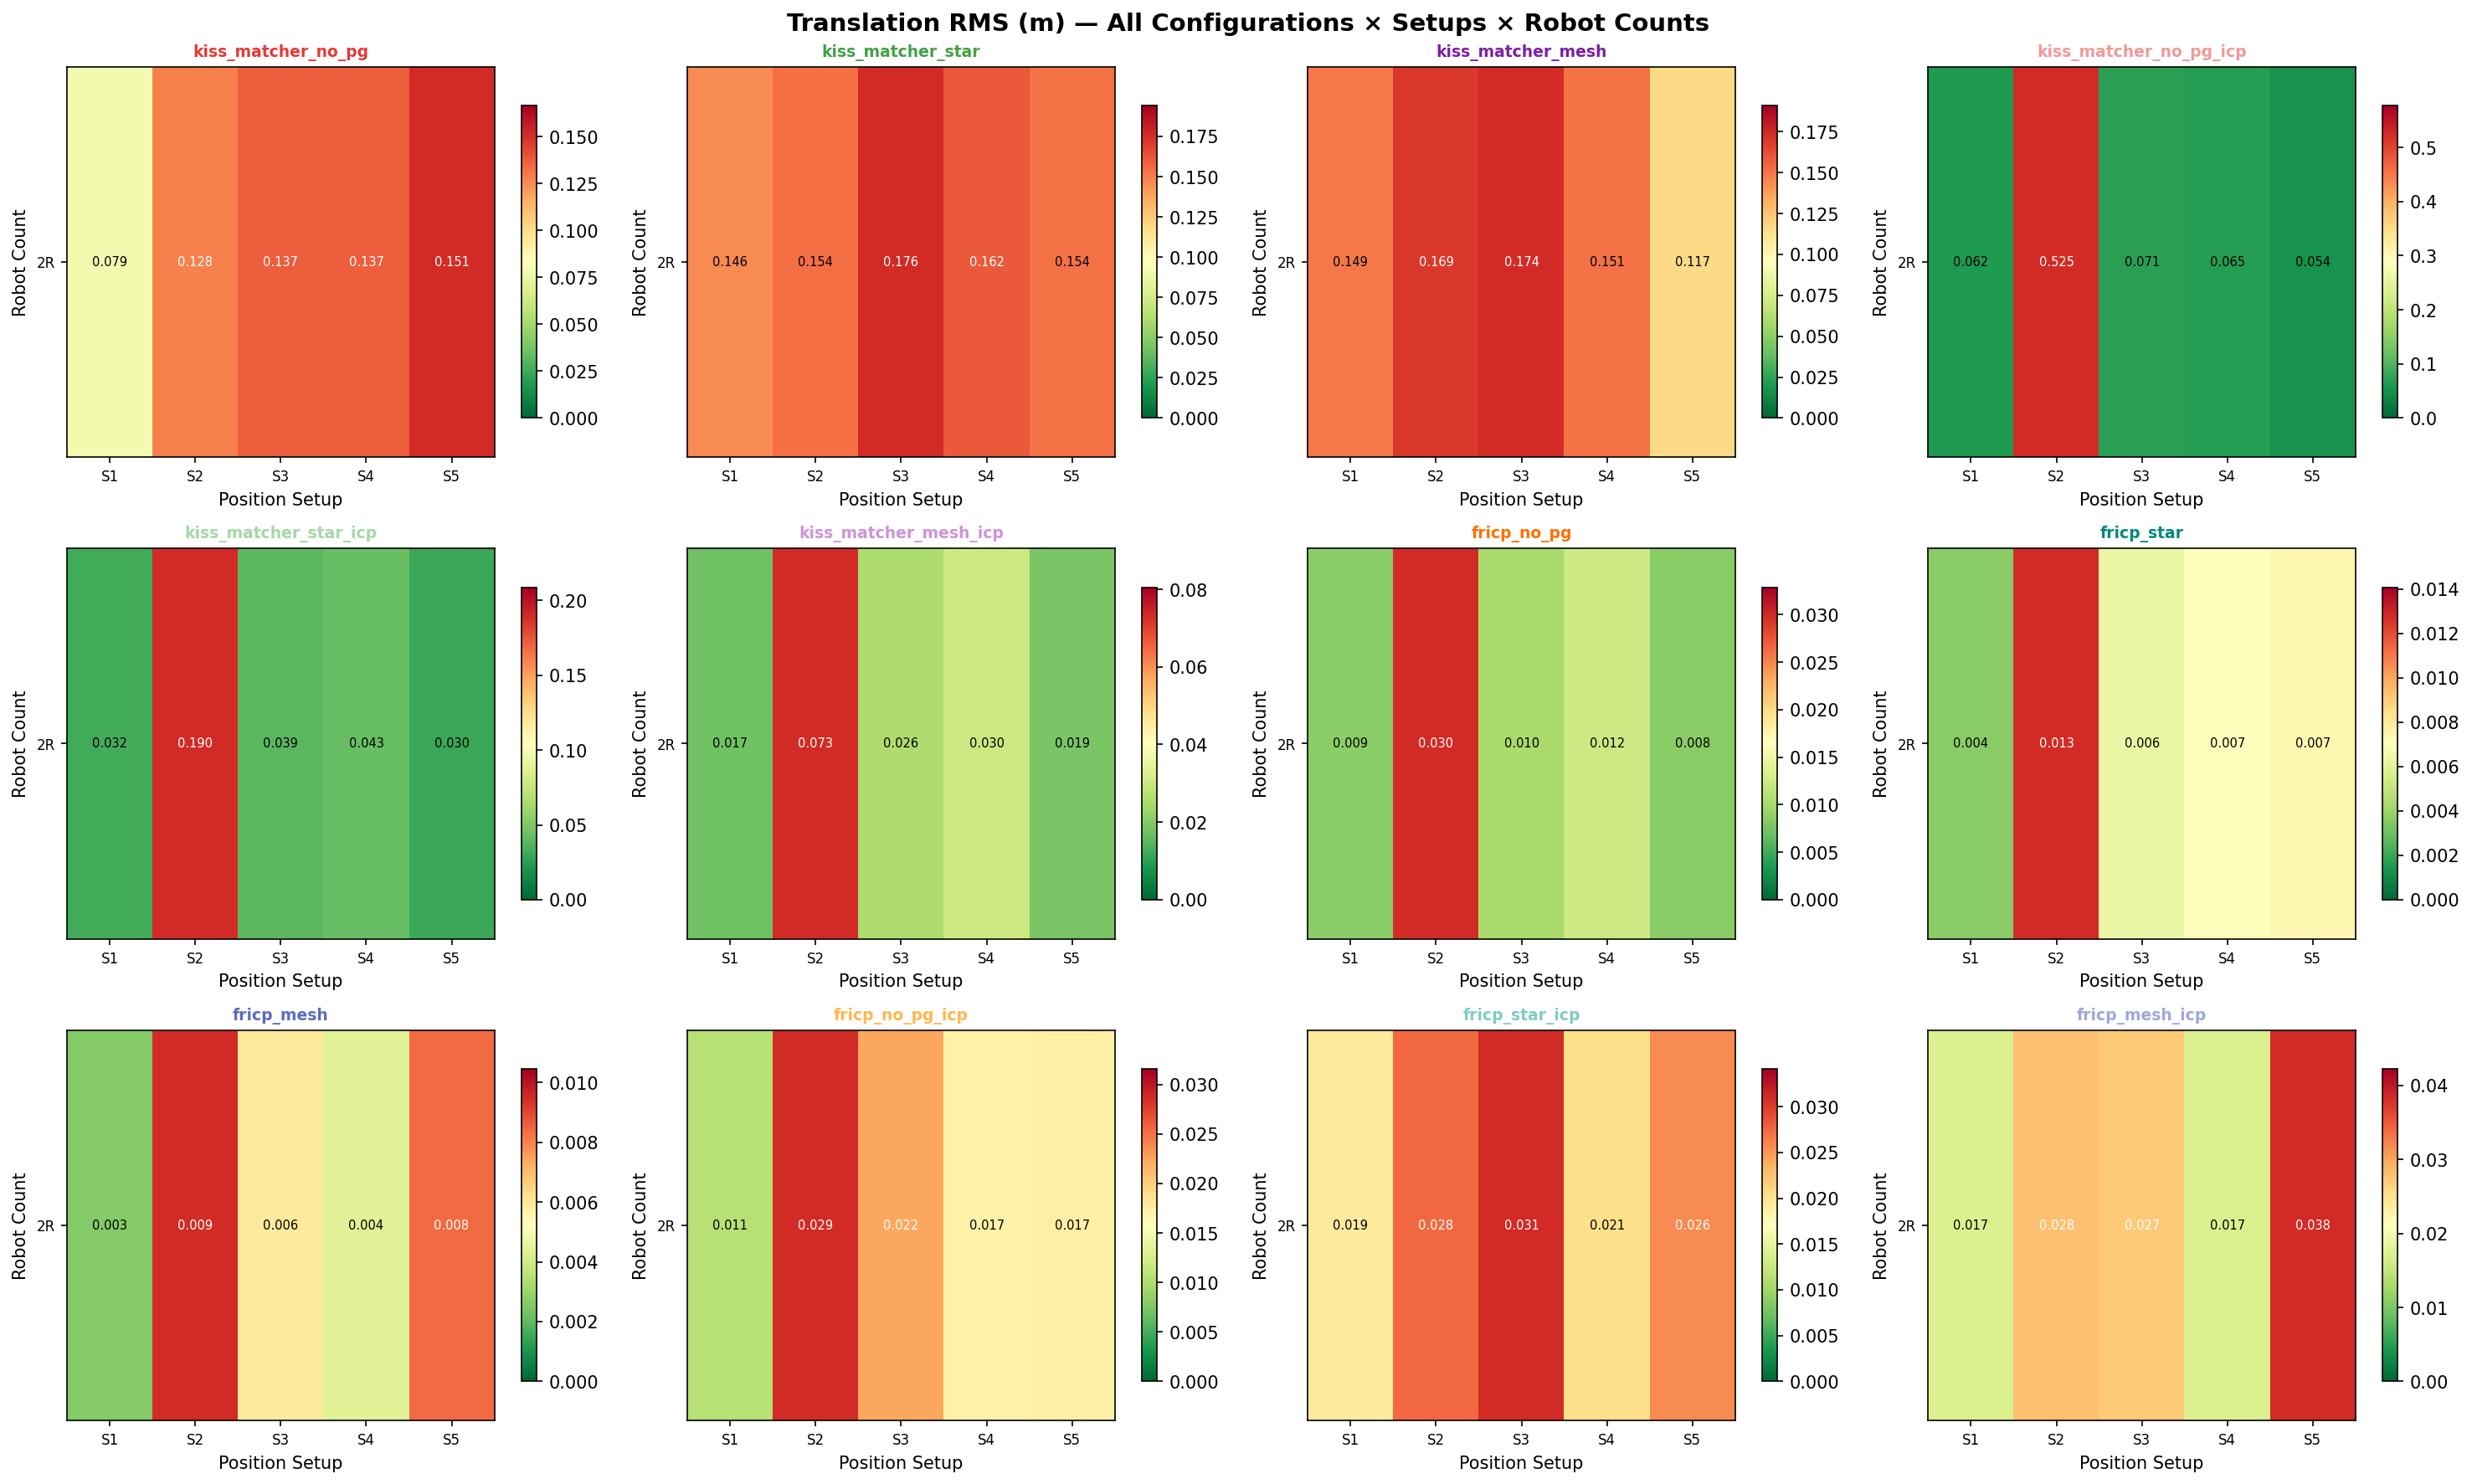
\includegraphics[width=\textwidth]{figures/heatmap_2_robots_proximity.png}
    \caption{Heatmap of translation error across position setups
             for all 12 configurations (2~robots, proximity).}
    \label{fig:app_2r_heatmap}
\end{figure}

\begin{figure}[htbp]
    \centering
    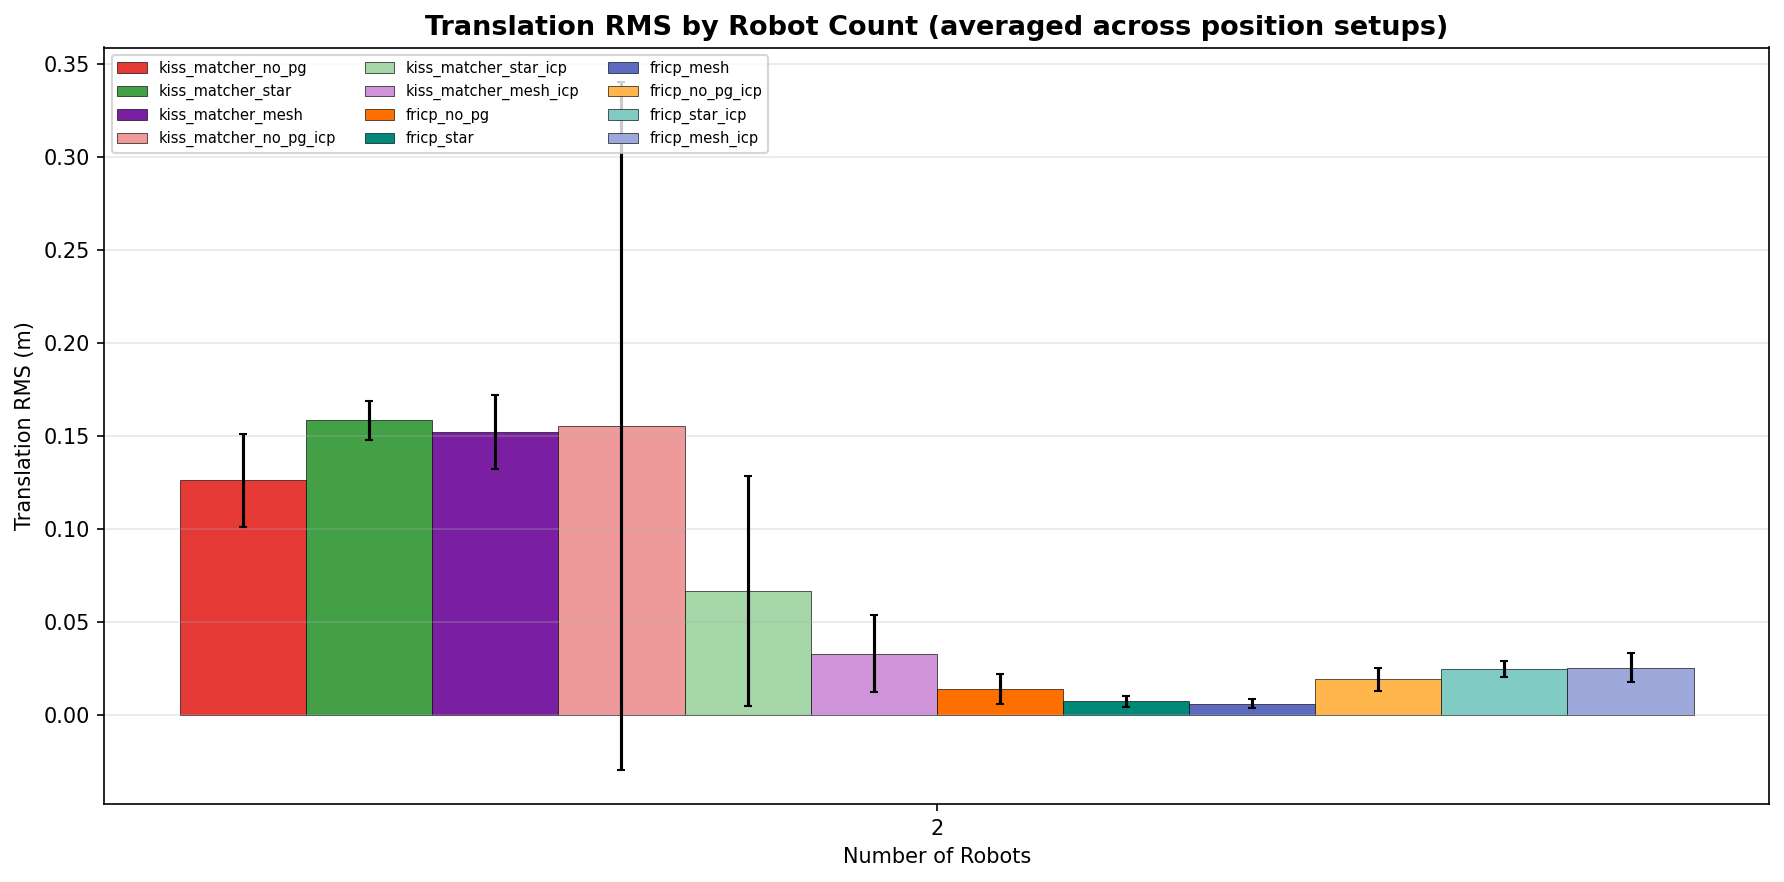
\includegraphics[width=\textwidth]{figures/summary_2_robots_proximity.png}
    \caption{Summary of translation error by configuration (2~robots, proximity).}
    \label{fig:app_2r_summary}
\end{figure}

%% ---------------------------------------------------------------------------
\section{Cross-Robot-Count Summary}
\label{sec:app_cross_count}

\begin{figure}[htbp]
    \centering
    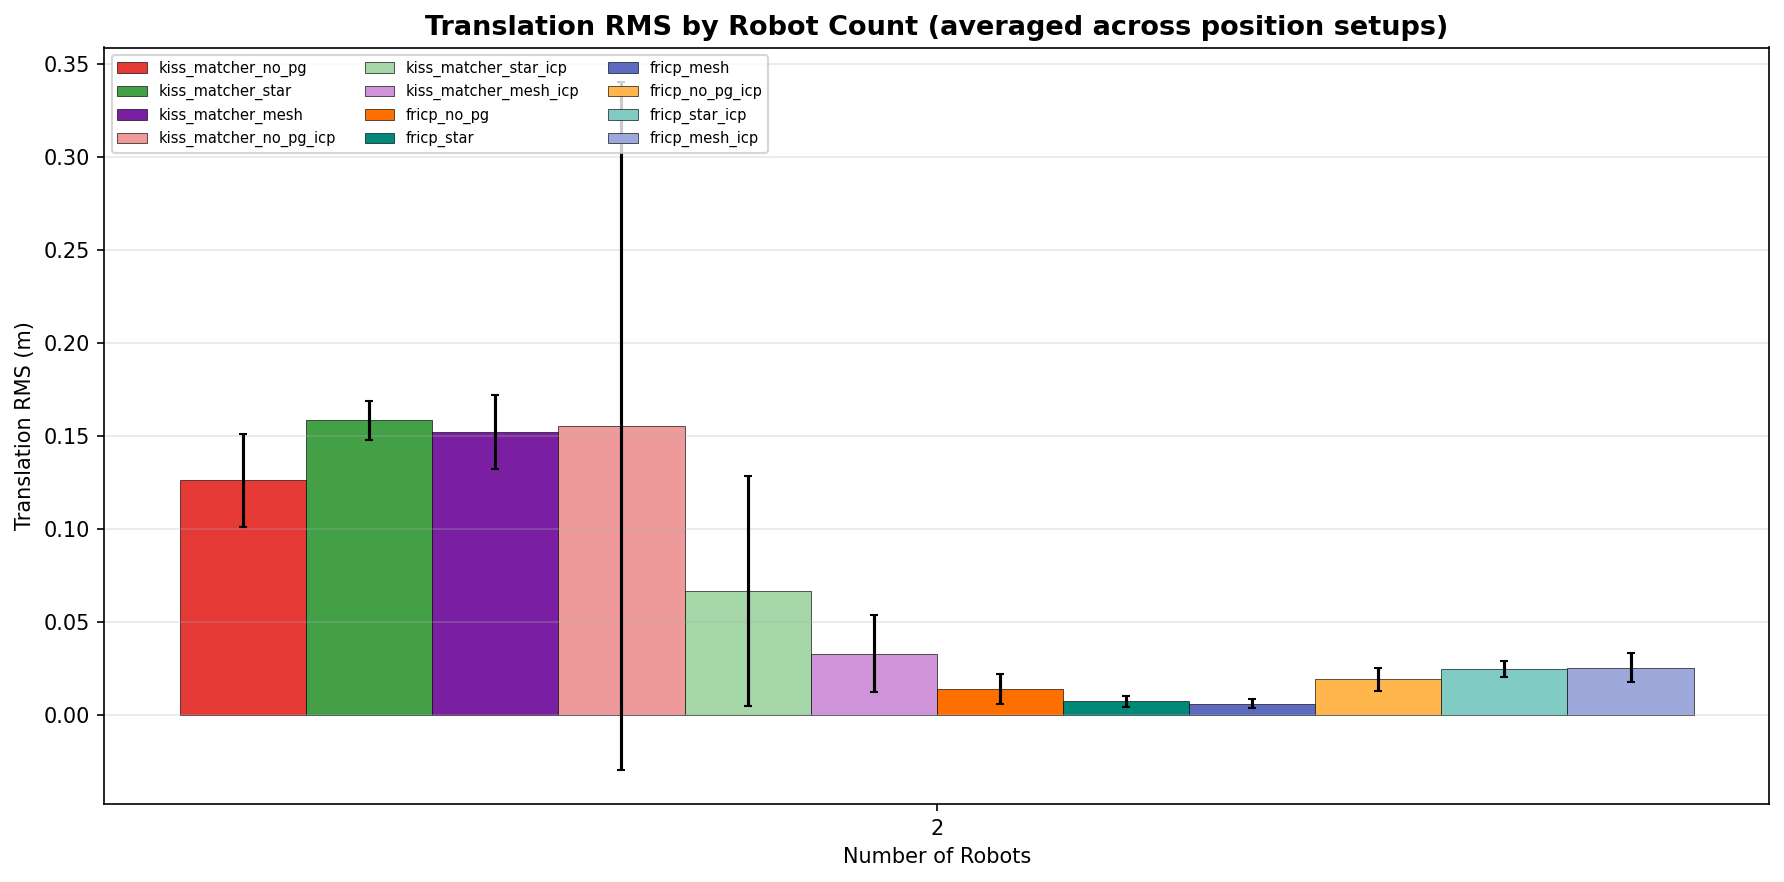
\includegraphics[width=\textwidth]{figures/summary_by_robot_count.png}
    \caption{Summary of translation RMS by robot count, grouped by
             configuration.}
    \label{fig:app_summary_by_count}
\end{figure}
